\documentclass[10pt]{beamer}
\mode<presentation>
\usepackage{amssymb,textcomp}
%\usepackage{beamerthemesplit}
\usepackage{beamerthemeBoadilla}
\usepackage{verbatim}
\usepackage{algorithm2e}
\usefonttheme{serif}
\title{Unidad III: Aproximaci\'on de funciones.}
\author{Jos\'e Luis Ram\'irez B.}
\date{\today}

\begin{document}

\frame{\titlepage}

\frame{\tableofcontents}

\section{Introducci\'on}
\begin{frame}[fragile]
  \frametitle{Motivaci\'on.} 
  \begin{itemize}
   \item<1-> En este tema se da una posible respuesta a una situaci\'on
bastante natural en el \'ambito cient\'ifico.
    \item<2-> Se Investiga un fen\'omeno que se est\'a desarrollando, se desea estudiarlo, y junto
con los modelos previos con que se cuente, se pueden tomar
muestras experimentales.
    \item<3-> Se tiene una serie de datos a partir de
mediciones sobre el mismo.
    \item<4-> Se desea extraer informaci\'on de esos datos.
  \end{itemize}
\end{frame}
%%%%%
\begin{frame}[fragile]
  \frametitle{Motivaci\'on.}
  Esencialmente podemos tratarlo con:
\begin{itemize}
 \item<2-> T\'ecnicas estad\'isticas (que continuar\'an observando el fen\'omeno de un modo discreto, es decir, sobre ese conjunto finito de mediciones).
 \item<3-> o bien ``intentando recrear/reconstruir el fen\'omeno en su totalidad'' (en un dominio continuo de espacio, tiempo o cualquier otra magnitud), con la funci\'on que represente ``lo mejor posible'' esos datos.
\end{itemize}
\end{frame}
%%%%%
%%%%
\frame
{
  \frametitle{Motivaci\'on.}
Las t\'ecnicas que utilizan funciones continuas y se consideran en este curso son de dos tipos:
\begin{itemize}
 \item<2-> Interpolaci\'on: c\'alculo de funciones que pasan (``interpolan'' es el t\'ermino matem\'atico) exactamente por los puntos dados.
 \item<3-> Curvas de ajuste: c\'alculo de funciones aproximadas a los datos que tenemos (en alg\'un sentido, para cierta distancia)
\end{itemize}
}
%%%%%
\frame{
%\footnotesize
\frametitle{Resultados Fundamentales}
\begin{block}{Polinomio de grado $n$:}
 $$p_n(x)=a_nx^n+a_{n-1}x^{n-1}+\cdots+a_1x+a_0\,(a_n \neq 0)$$
\end{block}
 
\uncover<2->
{\begin{block}{Teorema:}
Si $p_n$ es un polinomio de grado $n \geq 1$, entonces $p_n(x) = 0$ tiene al menos una ra\'iz (posiblemente compleja).
\end{block}}
}
%%%
\frame{
  \frametitle{Resultados Fundamentales}
\uncover<1->{
\begin{block}{Teorema:}
Sea $p_n$ un polinomio de grado $n \geq 1$, entonces existen constantes $x_1, x_2,\ldots,x_k$, posiblemente complejas, y enteros positivos $m_1, m_2, \ldots, m_k$, tales que $m_1 + m_2 + \ldots + m_k = n$ verificando:
$$
p_n(x) = a_n(x - x_1)^{m_1}(x - x_2)^{m_2}\cdots(x - x_k)^{m_k}
$$
\end{block}}
\uncover<2->{
\begin{block}{Teorema:}
Sean $p_n$ y $q_n$ dos polinomios de grado menor o igual que $n$. Si existen $x_1, x_2, \ldots, x_k,$ con $k > n$, n\'umeros distintos tales que $p_n(x_i) = q_n(x_i)$, $i = 1,\ldots , k$, entonces $p_n(x) = q_n(x)$ para todo $x$.
\end{block}}
}
%%%%
%%%%
\frame{  
\frametitle{Evaluaci\'on de polinomios}
\vspace{-0.5cm}
\footnotesize{
\begin{block}{$p_n(x)=a_nx^n+a_{n-1}x^{n-1}+\cdots+a_1x+a_0$}
Se necesitan menos operaciones para evaluarlo en un punto $x_0$ si se escribe:
$$
p_n(x) = a_0 + x(a_1 + x(\cdots(a_{n-2} + x(a_{n-1} + xa_n))\cdots))
$$
\end{block}}

\footnotesize{
\begin{block}{Algoritmo de Horner para evaluar $p_n(x_0)$}
\uncover<2->{
$$
\begin{array}{lr}
b_{n-1} = a_n\\
b_k = a_{k+1}+x_0b_{k+1} & k=n-2,\ldots,1,0,-1
\end{array}
$$
entonces: $p_n(x_0) = b_{-1}$}

\uncover<3->{
Adem\'as, si se llama
$$
q_{n-1}(x) = b_{n-1}x^{n-1}+b_{n-2}x^{n-2}+\cdots+b_1x+b_0
$$
se tiene que:
$$
p_n(x) = (x-x_0)q_{n-1}(x)+b_{-1}
$$
y por lo tanto
$$
p'_n(x_0) = q_{n-1}(x_0)
$$}
\end{block}}
}
%%%%
\frame{
\frametitle{Evaluaci\'on de polinomios}
\textquestiondown Por qu\'e es Importante el Algoritmo de Horner?
\begin{itemize}
 \item<2-> Eficiencia: Es m\'as eficiente que calcular las potencias de 
 $x_0$ y multiplicar por los coeficientes de forma individual (se usa 
 menos memoria y tiempo de c\'omputo).
 \item<3-> Estabilidad: Reduce errores de redondeo en c\'alculos num\'ericos.
 \item<4-> Derivadas: Permite obtener informaci\'on sobre la derivada del polinomio 
 en el mismo punto.
 \item<5-> Divisi\'on Sint\'etica: Est\'a relacionado con el m\'etodo de divisi\'on sint\'etica
 para polinomios, lo que lo hace muy \'util en el campo del \'algebra y el an\'alisis num\'erico.
\end{itemize}
}
%%%%
\frame{
\frametitle{Evaluaci\'on de polinomios}
En Resumen:
\begin{itemize}
\item El algoritmo de Horner es una herramienta poderosa para evaluar polinomios y 
tambi\'en para obtener informaci\'on sobre su derivada.
\item Es un m\'etodo eficiente, estable y muy utilizado en diversos campos de las matem\'aticas y la inform\'atica.
\end{itemize} 
}
%%%%%
\frame{
\frametitle{Ejemplo: Polinomio de Grado 3}

Tenemos el polinomio:
$$
p_3(x) = 2x^3 - 3x^2 + 4x - 1
$$
Y queremos evaluarlo en $x_0 = 2$ y tambi\'en calcular $p'_3(2)$.
}
\frame{
\frametitle{Ejemplo: Polinomio de Grado 3}
\begin{enumerate}
\item[1.] Aplicaci\'on del Algoritmo de Horner para $p_3(2)$

Recordemos que el algoritmo es:
\begin{block}{}
$$
\begin{array}{l}  
b_{n-1} = a_n\\
b_k = a_{k+1} + x_0 \cdot b_{k+1} \text{ para }k = n-2, ..., 1, 0, -1\\
p_n(x_0) = b_{-1}
\end{array}
$$
\end{block}
\begin{itemize}
  \item<2-> Inicializaci\'on:\\
$b_2 = a_3 = 2$ (coeficiente de $x^3$)
\item<3-> Iteraci\'on:\\
$b_1 = a_2 + x_0 \cdot b_2 = -3 + 2 \cdot 2 = 1$ (coeficiente de $x^2$)\\
$b_0 = a_1 + x_0 \cdot b_1 = 4 + 2 \cdot 1 = 6$ (coeficiente de $x^1$)\\
$b_{-1} = a_0 + x_0 \cdot b_0 = -1 + 2 \cdot 6 = 11$ (t\'ermino independiente)
\item<4-> Resultado:\\
$p_3(2) = b_{-1} = 11$
\end{itemize}
\end{enumerate}
}
%%%%%
\frame{
\frametitle{Ejemplo: Polinomio de Grado 3}
\begin{enumerate}
\item[2.] Obtención del Polinomio Cociente $q_2(x)$\\
Con los valores de $b$ que obtuvimos (excepto $b_{-1}$), podemos formar el polinomio cociente de grado 2:
$$
q_2(x) = b_2 x^2 + b_1 x + b_0 = 2x^2 + 1x + 6
$$
\item[3.]<2-> Relaci\'on entre $p_3(x)$, $q_2(x)$ y $b_{-1}$\\
El polinomio $p_3(x)$ se puede expresar como:\\
$p_3(x) = (x - x_0) \cdot q_2(x) + b_{-1}$\\
$p_3(x) = (x - 2) \cdot (2x^2 + x + 6) + 11$
\end{enumerate}
}
%%%%%
\frame{
\frametitle{Ejemplo: Polinomio de Grado 3}
\begin{enumerate}
\item[4.]<1-> Aplicaci\'on del Algoritmo de Horner a $q_2(x)$ para obtener $q_2(2) = p'_3(2)$

Aplicando el algoritmo de Horner para evaluar el polinomio $q_2(x)$ en $x_0 = 2$. Los coeficientes de $q_2(x)$ son: $b_2=2$, $b_1=1$, $b_0=6$

Llamemos a los nuevos coeficientes $c_i$:
\begin{itemize}
\item<2->Inicializaci\'on:\\
$c_1 = b_2 = 2$
\item<3->Iteraci\'on:\\
$c_0 = b_1 + x_0 \cdot c_1 = 1 + 2 \cdot 2 = 5$\\
$c_{-1} = b_0 + x_0 \cdot c_0 = 6 + 2 \cdot 5 = 16$
\item<4-> Resultado:\\
$q_2(2) = c_{-1} = 16$
\end{itemize}
\end{enumerate}
}
%%%%
\frame{
\frametitle{Ejemplo: Polinomio de Grado 3}
\begin{enumerate}
\item[5.]<1-> Derivada $p'_3(2)$\\
Se tiene que\\
$p'_3(2) = q_2(2) = 16$
\end{enumerate}
En resumen:
\begin{itemize}
\item<2-> $p_3(2) = 11$
\item<3-> $q_2(x) = 2x^2 + x + 6$
\item<4-> $p_3(x) = (x - 2) * (2x^2 + x + 6) + 11$
\item<5-> $p'_3(2) = q_2(2) = 16$
\end{itemize}
}
%%%%%
\frame{
\frametitle{Ejemplo: Polinomio de Grado 3}
{\bf Comprobaci\'on de la Derivada}

Derivando el polinomio $p_3(x)$ y evalu\'andolo en $x = 2$.
\begin{block}{}
$$
\begin{array}{l}
p_3(x) = 2x^3 - 3x^2 + 4x - 1\\
p'_3(x) = 6x^2 - 6x + 4
\end{array}
$$
\end{block}
\uncover<2->{
Evaluando en x = 2:
$$
p'_3(2) = 6(2^2) - 6(2) + 4 = 6(4) - 12 + 4 = 24 - 12 + 4 = 16
$$
}
}
%%%%
\section{Interpolaci\'on}
\subsection{Taylor}
\frame{
\frametitle{Problema de interpolaci\'on de Taylor}
\uncover<1->
{
\begin{block}{Problema de interpolaci\'on de Taylor}
Dados un entero $n$ no negativo, un punto $x_0 \in \mathbb{R}$ y los valores $f(x_0),f'(x_0),\ldots,f^{(n)}(x_0)$ de una funci\'on y sus $n$ primeras derivadas en $x_0$, encontrar un polinomio $P(x)$ de grado $\leq n$ tal que
$$
P(x_0) = f(x_0), P'(x_0) = f'(x_0),\ldots, P^{(n)}(x_0) = f^{(n)}(x_0).
$$
\end{block}}
\uncover<2->{
\begin{block}{Teorema:}
El problema de interpolaci\'on de Taylor tiene soluci\'on \'unica, que se denomina polinomio de Taylor de grado $\leq n$ de la funci\'on $f$ en el punto $x_0$:
\[
\textstyle
P(x) = f(x_0)+f'(x_0)(x-x_0)+f''(x_0)\frac{(x-x_0)^2}{2!}+\cdots+f^{(n)}(x_0)\frac{(x-x_0)^n}{n!}
\]
\end{block}}
}
%%%%
\frame{
\frametitle{Problema de interpolaci\'on de Taylor}
\uncover<1->{
\begin{block}{Teorema:}
Para $n > 1$ sea $f(x)$ una funci\'on $n$ veces derivable en $x_0$. El polinomio de Taylor $P(x)$ verifica que:
$$
\lim_{x \to x_0}\frac{f(x)-P(x)}{(x-x_0)^n}=0
$$
con la notaci\'on $o$ peque\~na de Landau $f(x) - P(x) = o((x - x_0)^n)$ para $x \to x_0$. Adem\'as, $P(x)$ es el \'unico polinomio de grado $\leq n$ con esta propiedad.
\end{block}}
}
%%%%
\frame{
\frametitle{Problema de interpolaci\'on de Taylor}
\begin{itemize}
 \item Error del polinomio interpolador de Taylor
\uncover<2->{
\begin{block}{Teorema:}
Sean $x$ y $x_0$ dos n\'umeros reales distintos y $f(x)$ una funci\'on con $n$ derivadas continuas en un intervalo conteniendo a $x$ y $x_0$, en el que tambi\'en existe $f^{(n+1)}$. Entonces existe un punto $\xi$ entre $x$ y $x_0$ tal que:
$$
f(x)-P(x) = f^{(n+1)}(\xi)\frac{(x-x_0)^{n+1}}{(n+1)!}
$$
\end{block}}
\end{itemize}
}
%%%%
\frame{
\frametitle{Problema de interpolaci\'on de Taylor}
\begin{block}{Colorario:}
Adem\'as de las hip\'otesis del teorema supongase que para cada $t$ entre $x$ y $x_0$ se verifica que $|f^{(n+1)}(t)| \leq K_{n+1}$ constante, entonces:
$$
|f(x)-P(x)| \leq \frac{|x-x_0|^{(n+1)}K_{n+1}}{(n+1)!}
$$
\end{block}
}
%%%%
\frame{
\frametitle{Ejemplo:}
A continuaci\'on se muestran las gr\'aficas de la funci\'on $f(x) = \sin(x)$ y de su polinomio de Taylor de orden 1 al 9 en el cero. Se puede comprobar que la aproximaci\'on es m\'as exacta a medida que se aumenta el orden.
\begin{center}
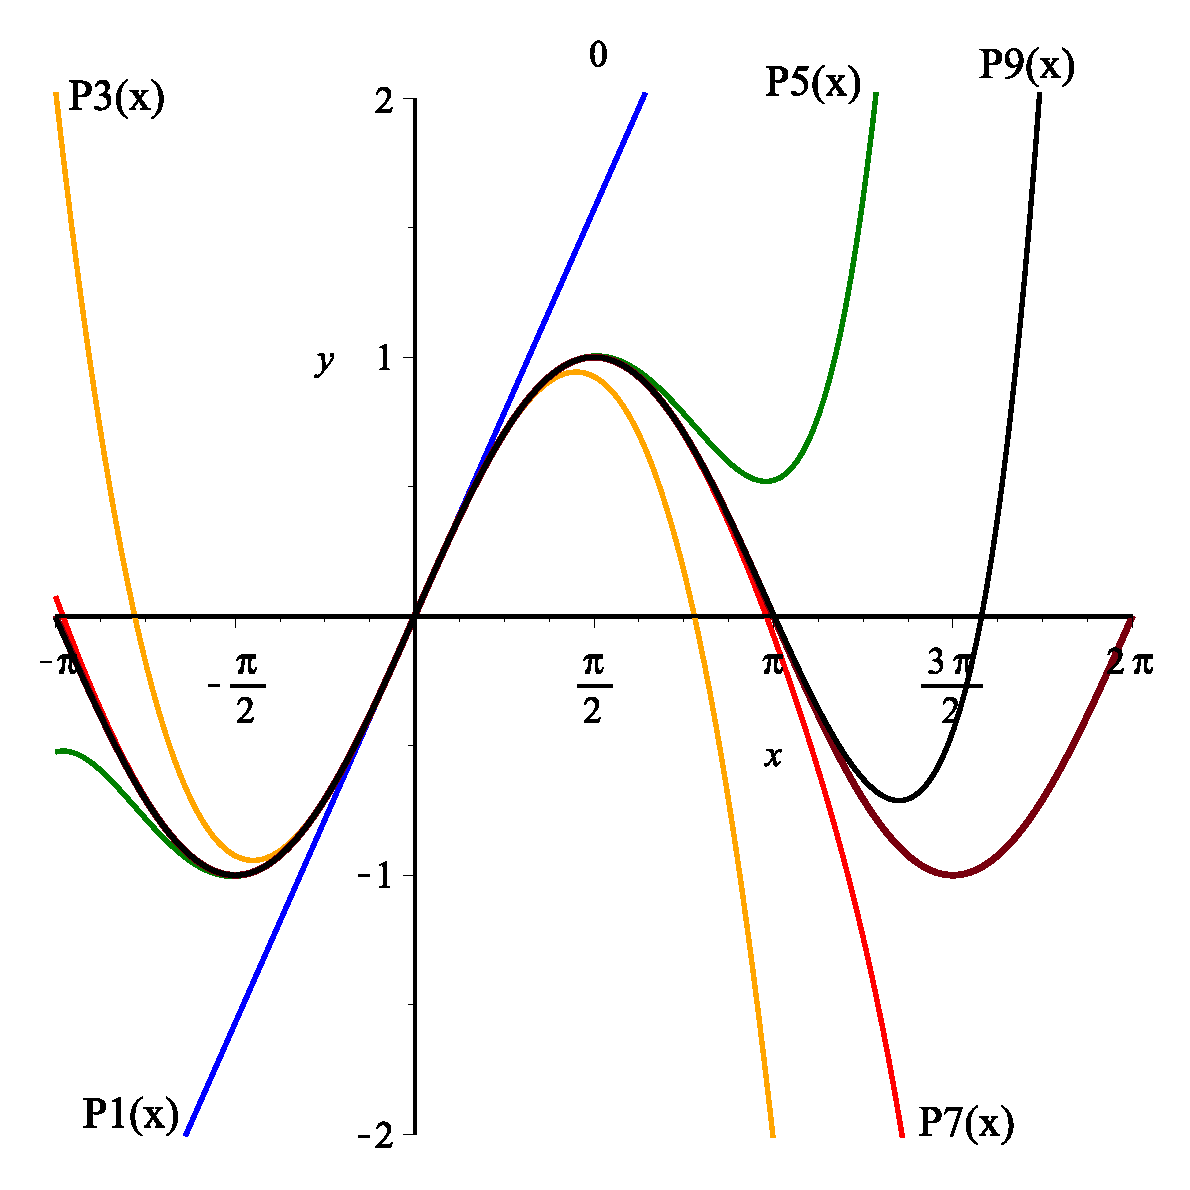
\includegraphics[scale=0.28]{taylorsin.eps}
\end{center}
}
%%%%
\frame{
\frametitle{Ejemplo:}
El hecho de que la funci\'on seno y su polinomio de Taylor se parezcan tanto como se quiera, con s\'olo aumentar el grado del polinomio lo suficiente, no es algo que le ocurra a todas las funciones. Para la funci\'on arctan la situaci\'on no es tan buena:
\begin{center}
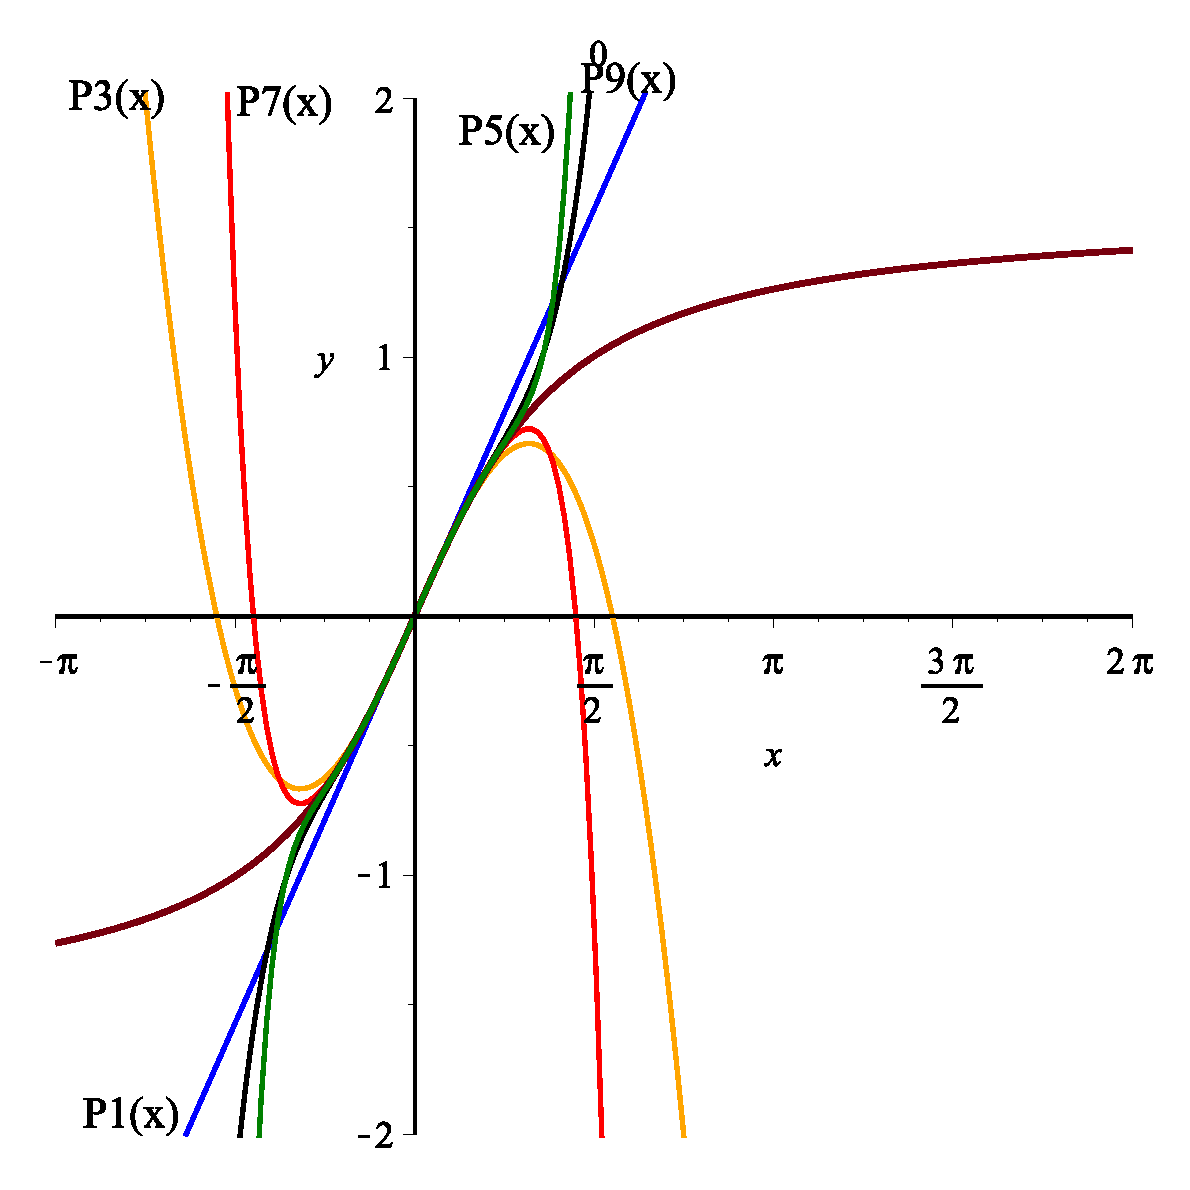
\includegraphics[scale=0.28]{tayloratan.eps}
\end{center}
}
%%%%%
\begin{frame}
  \frametitle{Ejemplo:}
  \begin{itemize}
    \item Se  desea aproximar la funci\'on $f(x)=e^x$ mediante el polinomio de Taylor centrado en $x_0=0$ de orden 5 y hallar el error obtenido en la estimaci\'on para $x=1.5$ 
   
    \item El polinomio de Taylor de grado 5 viene dada por la siguiente expresi\'on
    \begin{block}{}
    \scriptsize{
    $$
    \begin{array}{c}
      P_5(x) = 1+1(x-0)+\dfrac{1}{2!}(x-0)^2+\dfrac{1}{3!}(x-0)^3+\dfrac{1}{4!}(x-0)^4+\dfrac{1}{5!}(x-0)^5\\[10pt]
      P_5(x) = 1+x+\dfrac{1}{2!}x^2+\dfrac{1}{3!}x^3+\dfrac{1}{4!}(x-0)^4+\dfrac{1}{5!}x^5
    \end{array}
    $$}
    \end{block}
  \end{itemize}
\end{frame}
%%%%%
\begin{frame}
  \frametitle[short title]{Ejemplo:}
  Con la expresi\'on del residuo se calcula el error de Truncamiento:
  \begin{block}{}
    $$
    R_5(x) = \dfrac{f^{(6)}(\xi)}{6!}(x-x_0)^6=\dfrac{f^{(6)}(\xi)}{6!}x^6 = \dfrac{e^\xi}{6!}x^6
    $$
    $$
    R_5(x)=\dfrac{e^\xi}{6!}x^6
    $$
  \end{block}
\end{frame}
%%%%%
\begin{frame}
\frametitle{Ejemplo:}
 \begin{itemize}
   \item Ahora, vamos a aproximar $f(1.5) = e^{1.5}$ usando $P_5(1.5)$:\\
   $P_5(1.5) = 1 + 1.5 + \dfrac{(1.5)^2}{2} + \dfrac{(1.5)^3}{6} + \dfrac{(1.5)^4}{24} + \dfrac{(1.5)^5}{120}$
 \item<2-> Obtenemos:\\
   $P_5(1.5) \approx 4.462$
 \item<3-> C\'alculo del error en $x = 1.5$\\
 El error en la aproximaci\'on de Taylor est\'a dado por el t\'ermino del resto. La forma del resto para el polinomio de Taylor de orden $n$ es:\\
 $$
 R_n(x) = \dfrac{f^{(n+1)}(\xi)}{(n+1)!}(x-x_0)^{n+1}
 $$ 
 \end{itemize}
\end{frame}
%%%%%
\begin{frame}
\frametitle{Ejemplo:}
 \begin{itemize}
   \item<1-> En nuestro caso, $n = 5$, $x = 1.5$, $x_0 = 0$, y la derivada de orden 6 (o cualquiera) de $e^x$ es $e^x$.\\
   Por lo tanto:
   $$
   \begin{array}{l}
   R_5(1.5) = \dfrac{e^\xi \cdot (1.5 - 0)^6}{6!}\\[10pt]
   R_5(1.5) = \dfrac{e^\xi \cdot 1.5^6}{720} 
   \end{array}
   $$
   Donde $\xi$ es un n\'umero entre 0 y 1.5.
   \item<2-> Para maximizar el error, tomamos el mayor valor posible de $e^\xi$ en el intervalo [0, 1.5]. Este valor es cuando $c=1.5$.\\
Por lo tanto
$$
R_5(1.5) = e^{1.5} \cdot \dfrac{(1.5)^6}{720} \approx 0.0708
$$
 \end{itemize}
\end{frame}
%%%%
\frame{
\frametitle{Ejemplo:}
 \begin{itemize}
   \item<1-> C\'alculo del Valor Real y el Error Exacto

   \item<2-> El valor real de $e^{1.5}$ es aproximadamente 4.481689.
   
   \item<3-> El error exacto es:
   $$
   \begin{array}{l}
   \text{Error} = |e^{1.5} - P_5(1.5)|\\[10pt]
   \text{Error} = |4.481689 - 4.462 |\\[10pt]
   \text{Error} = 0.019689
   \end{array}
   $$
  \end{itemize}
}
%%%%
\subsection{Lagrange}
\frame
{
\frametitle{Interpolaci\'on}
\begin{itemize}
 \item<1-> Nos centraremos ahora en el problema de obtener, a partir de una tabla de parejas $(x,f(x))$ definida en un cierto intervalo $[a,b]$, el valor de la funci\'on para cualquier $x$ perteneciente a dicho intervalo.
 
 \item<2-> Supongamos que se dispone de las siguientes parejas de datos:
$$
\begin{array}{|c|c|c|c|c|c|}\hline
  \textbf{x} & x_0 & x_1 & x_2 & \cdots & x_n\\\hline
  \textbf{y} & y_0 & y_1 & y_2 & \cdots & y_n\\\hline
 \end{array}
$$
\end{itemize}
}
%%%%
\frame
{
  \begin{itemize}
    \item El objetivo es hallar una funci\'on continua lo m\'as sencilla posible tal que:
    \begin{block}{}
    $$
      \widetilde{f}(x_k) = y_k = f(x_k) \quad\forall k = 0,\ldots,n
    $$
    \end{block}
    en donde $x_k$ y $f(x_k)$ son datos conocidos.

    \item<2->Se dice entonces que la funci\'on $\widetilde{f}(x)$ , es una funci\'on interpolante de los datos representados en la tabla.
    \uncover<3->{\begin{block}{Observaci\'on:}
      En general, trabajaremos con $f$ = polinomios de grado $\leq n$
      $$
      P(x) = a_nx^n + a_{n-1}x^{n-1} + \cdots + a_1x + a_0
      $$
      polinomio algebraico
      \end{block}}
\end{itemize}
}
%%%%
\frame
{
\begin{figure}
 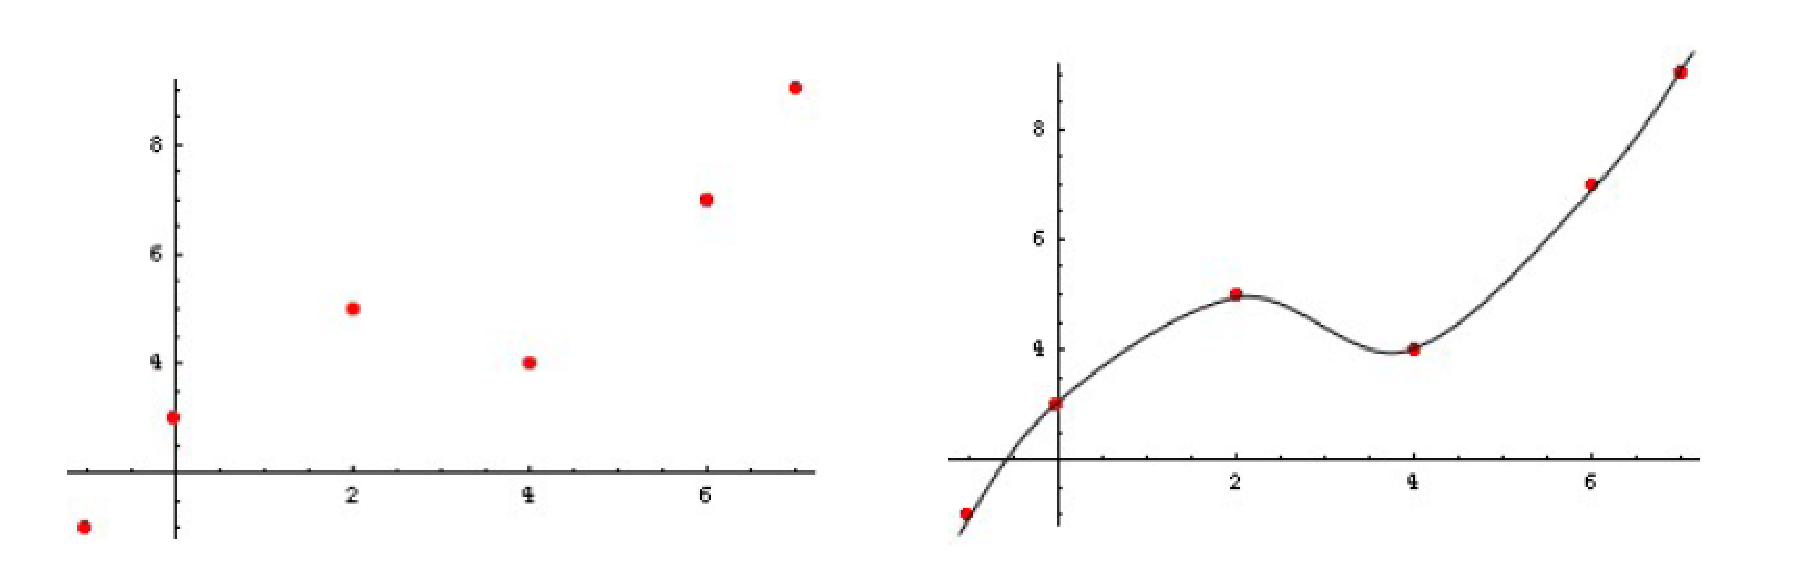
\includegraphics[scale=0.37]{img1.eps}
 \caption{Datos de iterpolaci\'on y curva interpolante.}
\end{figure}
}
%%%
\frame
{
\begin{block}{Teorema de Weierstrass:}
Sea $f$ continua sobre $[a,b]$, dado $\varepsilon > 0 \quad \exists P(x)$ polinomio tal que $\mid f(x)-P(x)\mid < \varepsilon \quad \forall x\in [a,b]$.
\end{block}
}
%%%%%
\frame
{
\frametitle{Polinomio interpolador de Lagrange}
\begin{itemize}
\item Si se escribe $P(x) = a_0 + a_1x + \cdots + a_nx^n$. As\'i, $P(x)$ ser\'a soluci\'on del problema si, y s\'olo si, el S.E.L:
\begin{block}{}
$$
\left(
\begin{array}{ccccc}
 1 & x_0 & x_0^2 & \cdots & x_0^n\\
 1 & x_1 & x_1^2 & \cdots & x_1^n\\
 1 & x_2 & x_2^2 & \cdots & x_2^n\\
 1 & \vdots & \vdots & \ddots & \vdots\\
 1 & x_n & x_n^2 & \cdots & x_n^n\\
\end{array}\right)
\left(
\begin{array}{c}
 a_0\\
 a_1\\
 a_2\\
 \vdots\\
 a_n\\
\end{array}\right) =
\left(
\begin{array}{c}
 y_0\\
 y_1\\
 y_2\\
 \vdots\\
 y_n\\
\end{array}
\right)
$$
\end{block}
admite soluci\'on.

\item<2-> que se denomina sistema cuadrado de Vandermonde. La matriz $A$ del sistema se denomina matriz de Vandermonde y es no-singular si los puntos $x_0, x_1, \ldots , x_n$ son diferentes. Esta matriz es mal condicionada a medida que $n$ aumenta.
\end{itemize}
}
%%%%%
\begin{frame}
  \frametitle{Polinomio interpolador de Lagrange}
  \begin{itemize}
    \item Llamando $A$ a la matriz de coeficientes del sistema; se tiene que el problema de interpolaci\'on admite una \'unica soluci\'on si, y s\'olo si, los nodos de interpolaci\'on son distintos. Para ello basta con probar que $\det(A) = \prod_{i>j}(x_i-x_j)$ y, por lo tanto, $\det(A) \neq 0 \Leftrightarrow x_i \neq x_j$.
    \item<2-> El m\'etodo de Lagrange para interpolaci\'on polinomial resulta de resolver este sistema para obtener los coeficientes pero lo hace de una forma m\'as sencilla y sistem\'atica. 
  \end{itemize}
\end{frame}
%%%%%
\frame{
\frametitle{Interpolaci\'on de Lagrange}
Para calcular el polinomio interpolador $P(x)$ asociado a una tabla de datos $(x_i, y_i)$ con $i =0,\ldots,n$ se puede plantear una simplificaci\'on previa: se construyen polinomios $l_i(x)$ de grado $n$ que valgan 1 en el nodo $x_i$ y 0 en el resto.

\begin{block}{}
$$
l_i(x_k) = \delta_{ik}=\left\{
\begin{array}{ccc}
 1 & \textrm{si} & i=k\\
 0 & \textrm{si} & i\neq k
\end{array}
\right.
$$
\end{block}
\uncover<2->{Si se escribe el polinomio factorizado para que tenga en
cada nodo $x_j$ (con $j \neq i$) una ra\'iz, el candidato es:
\begin{block}{}
$$
(x - x_0)(x - x_1)\cdots (x - x_{i-1})(x - x_{i+1}) \cdots (x - x_n) = \prod_{j=0,j\neq i}^n(x - x_j)
$$
\end{block}}
}
%%%
\frame
{\frametitle{Polinomio interpolador de Lagrange}
Lo \'unico que no se consigue es que en $x_i$ valga 1, para ello hay que ``normalizar'' la funci\'on anterior.

\uncover<2->{As\'i, finalmente la f\'ormula de interpolaci\'on de Lagrange es:
\begin{block}{}
$$
P(x) = \sum_{k=0}^n y_kl_k(x), \quad l_k(x) = \prod_{j=0,j\neq k}^n\frac{x - x_j}{x_k - x_j}, k=0,\ldots,n
$$
\end{block}
Los polinomios $l_k(x)$ reciben el nombre de polinomios de Lagrange.}
}
%%%%%
\begin{frame}
  \frametitle{Interpolaci\'on de Lagrange}
\begin{block}{Teorema:}
  Sean $x_0, x_1, \ldots , x_n$, $n + 1$ n\'umeros diferentes, y sea $f$ una funci\'on tal que
sus valores se obtengan a partir de los n\'umeros dados $(f(x_0), f(x_1), \ldots , f(x_n))$, entonces
existe un \'unico polinomio $p_n(x)$ de grado $n$, que cumple con la propiedad
$$
f(x_k) = p_n(x_k) \text{ para cada }k = 0,1, \ldots , n
$$
y este polinomio est\'a dado por la siguiente expresi\'on
\small{
$$
p_n(x) = f(x_0)L_0(x) + f(x_1)L_1(x) + \cdots + f(x_n)L_n(x) = \sum_{k=0}^nf(x_k)L_k(x)
$$}
\end{block}
\end{frame}
%%%%%
\begin{frame}
  \frametitle{Interpolaci\'on de Lagrange}
  Demostraci\'on:
  \begin{itemize}
    \item Se tiene que $p_n(x)=L_0(x)f(x_0)+L_1(x)f(x_1)+\cdots+L_n(x)f(x_n)$ ya que $L_k(x)$ 
    son polinomios de grado menor o igual a $n$ esto implica que $p(x)$ es un polinomio de grado menor o igual a $n$.
    \item<2-> Adem\'as
    $$
    \begin{array}{l}
    L_k(x_k) = 1,\quad L_k(x_j) =0 \mbox{ si $j \neq k$}\\
    \text{\small $\Rightarrow p_n(x_k) = 0 + 0 + \cdots + f(x_k) + \cdots + 0 = f(x_k) \quad \forall k=0,1,\ldots,n$}
    \end{array}
    $$
  \end{itemize}
\end{frame}
%%%%%
\begin{frame}
  \frametitle{Interpolaci\'on de Lagrange}
  \begin{itemize}
    \item La unicidad puede demostrarse como sigue:
    
    \item<2-> Supongase que $p_n(x)$ y $q_n(x)$ son dos polinomios de grado $\leq n$ que interpolan a $f(x)$ en los $n+1$ 
    puntos distintos $x_k,\quad k = 0,\ldots, n$, es decir
    $$
    p_n(x_k) = q_n(x_k) = f(x_k), \qquad k=0,1 \ldots,n
    $$
    \uncover<3->{
    Entonces, $r_n(x) = p_n(x)-q_n(x)$ es un polinomio de grado $\leq n$ con $n+1$ raices $x_0, x_1, \ldots, x_n$. Pero cualquier polinomio de grado $n$ con un n\'umero de raices mayor a $n$ debe ser constante e igual a cero. Por lo tanto $r_n (x) \equiv 0, \forall x$, y en consecuencia $p_n (x) = q_n (x), \forall x \in [a, b]$.}
  \end{itemize}
\end{frame}
%%%%
\frame
{
\frametitle{Polinomio interpolador de Lagrange}
Si $x_0,\ldots,x_n$ son $n+1$ n\'umeros reales distintos y $f$ es una funci\'on real definida sobre ellos, entonces existe un \'unico polinomio $P_n(x)$ de grado menor o igual a $n$ tal que
$f(x_k)=P(x_k)\quad \forall k=0,\ldots,n$.

\uncover<2->{
  \begin{block}{Teorema}
  
    Si $f \in \mathcal{C}^{n+1} [a, b]$ y $p_n(x)$ es el polinomio de interpolaci\'on en $n+1$ puntos distintos $x_0 = a, 
    x_1 , \ldots , x_n = b$, entonces para cada $x \in [a, b]$ existe $\xi(x) \in I[x_0 , x_1 , . . . , x_n , x]$ (el 
    intervalo cerrado m\'as peque\~no que contiene $x_0 , x_1 , \ldots , x_n , x$) tal que
    $$
   f(x) - p_n(x) = \dfrac{f^{(n+1)}(\xi(x))}{(n+1)!}w(x) \qquad \mbox{con } w(x) = \prod_{j=0}^n(x-x_j)
   $$
   \end{block}
}
}
%%%%%%
\frame{
  \frametitle{Polinomio interpolador de Lagrange}
  \underline{Demostraci\'on:} 
  \begin{itemize}
    \item<2-> Si $x = x_k$ para alg\'un $0 \leq k \leq n$, la igualdad se satisface trivialmente 
pues ambos lados son iguales a cero. 
\item<3->As\'i que supongase que $x \neq x_k , k = 0, 1, \ldots , n$, y sea 
$$
F(t) = f(t)-p_n(t) - \dfrac{f(x)-p_n(x)}{w(x)}w(t), \qquad t \in [a,b]
$$
\item<4->Claramente $F(t)$ est\'a bien definida pues $w(x) \neq 0$ ya que $x \neq x_k , \forall k$. Adem\'as $F(t)$ es de
clase $\mathcal{C}^{n+1} [a,b]$ y tiene al menos $n + 2$ ceros, a saber $x_0 , x_1 , \ldots, x_n , x$. Luego $F'(t)$ 
tiene al menos $n + 1$ ceros, $F''(t)$ tiene al menos $n$ ceros, as\'i sucesivamente, y $F^{(n+1)}(t)$ tiene al menos 
un cero en $[a,b]$ que ser\'a denotado por $\xi(x)$. 
\end{itemize}
}
%%%%%
\frame{
\frametitle{Polinomio interpolador de Lagrange}
\begin{itemize}
\item Por lo tanto
$$
0 = F^{(n+1)}(\xi(x)) = f^{(n+1)}(\xi(x)) - 0 -\dfrac{f(x)-p_n(x)}{w(x)}(n+1)!
$$
\uncover<2->{  
Se concluye que
\begin{block}{}
$$
f(x) - p_n(x) = \dfrac{f^{(n+1)}(\xi(x))}{(n+1)!}w(x)	
$$}
\end{block}
\end{itemize}
}
%%%
\frame{
\frametitle{Ejemplo:}
Sea la funci\'on $f:x\rightarrow2xe^{-(4x+2)}$ definida en $[0.2, 1]$
\begin{enumerate}
 \item<2-> Calcular y representar gr\'aficamente los polinomios de base de Lagrange asociados al soporte $\{0.2, 1.0\}$.
 \item<3-> Hallar el polinomio $P(x)$ que interpola $f(x)$ en el sentido de Lagrange sobre el soporte $\{0.2, 1\}$.
 \item<4-> Obtener la expresi\'on del error de interpolaci\'on.
 \item<5-> Hallar una cota de error v\'alida en todo $(0.2, 1)$.
\end{enumerate}
}
%%%
\frame
{
\frametitle{Ejemplo:}
$$
\begin{array}{cc}
 l_0(x)=\frac{x-x_1}{x_0-x_1}=\frac{1-x}{0.8} & l_1(x)=\frac{x-x_0}{x_1-x_0}=\frac{x-0.2}{0.8}\\
 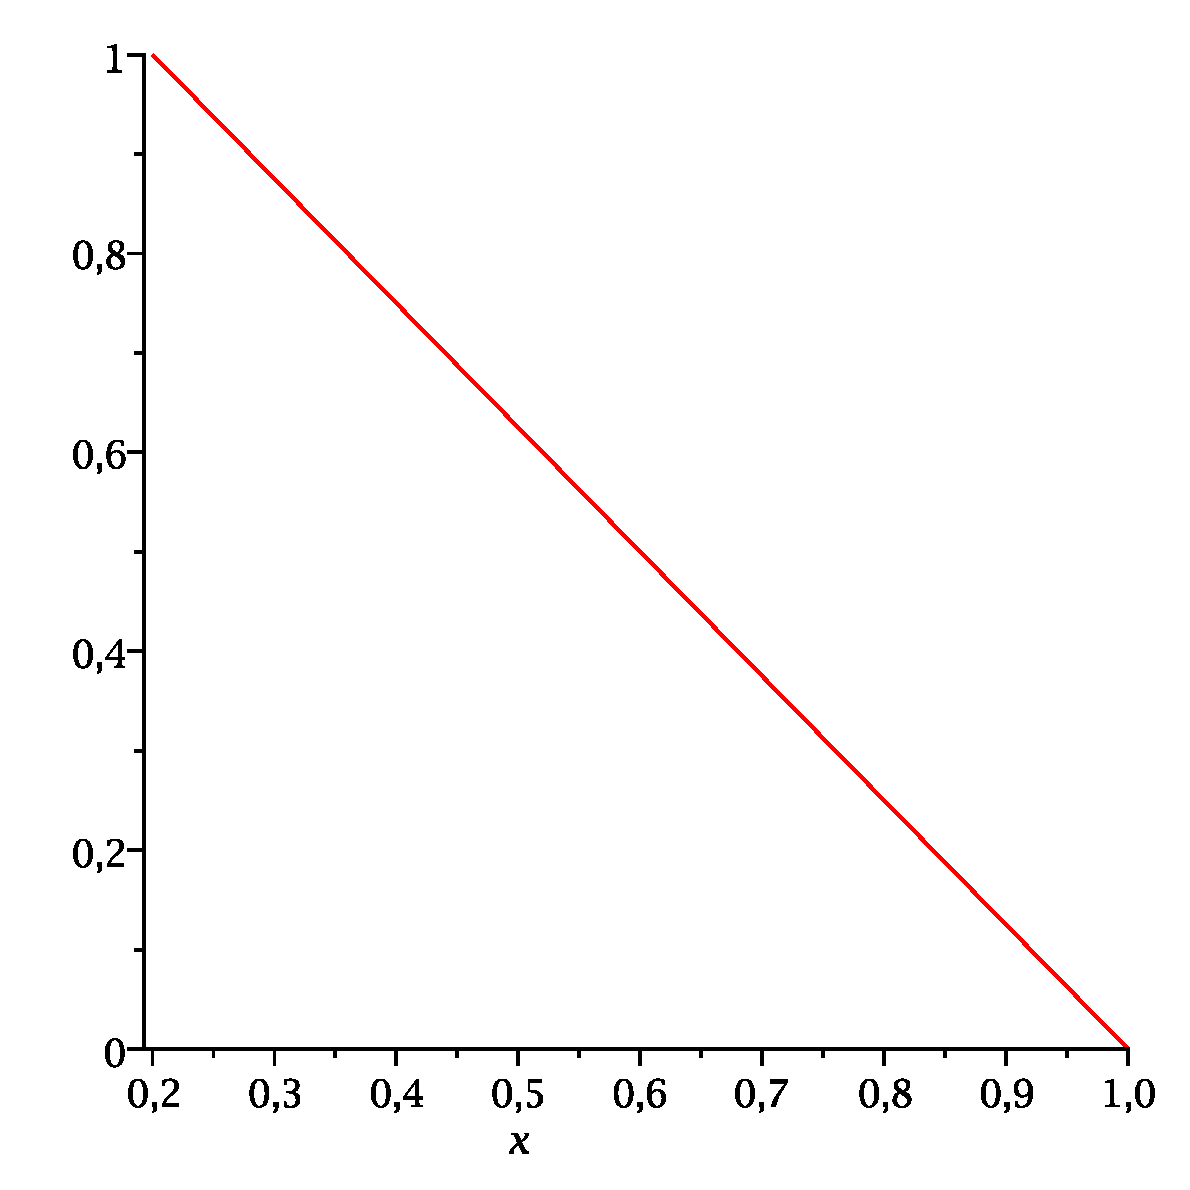
\includegraphics[scale=0.25]{soporte1.eps} & 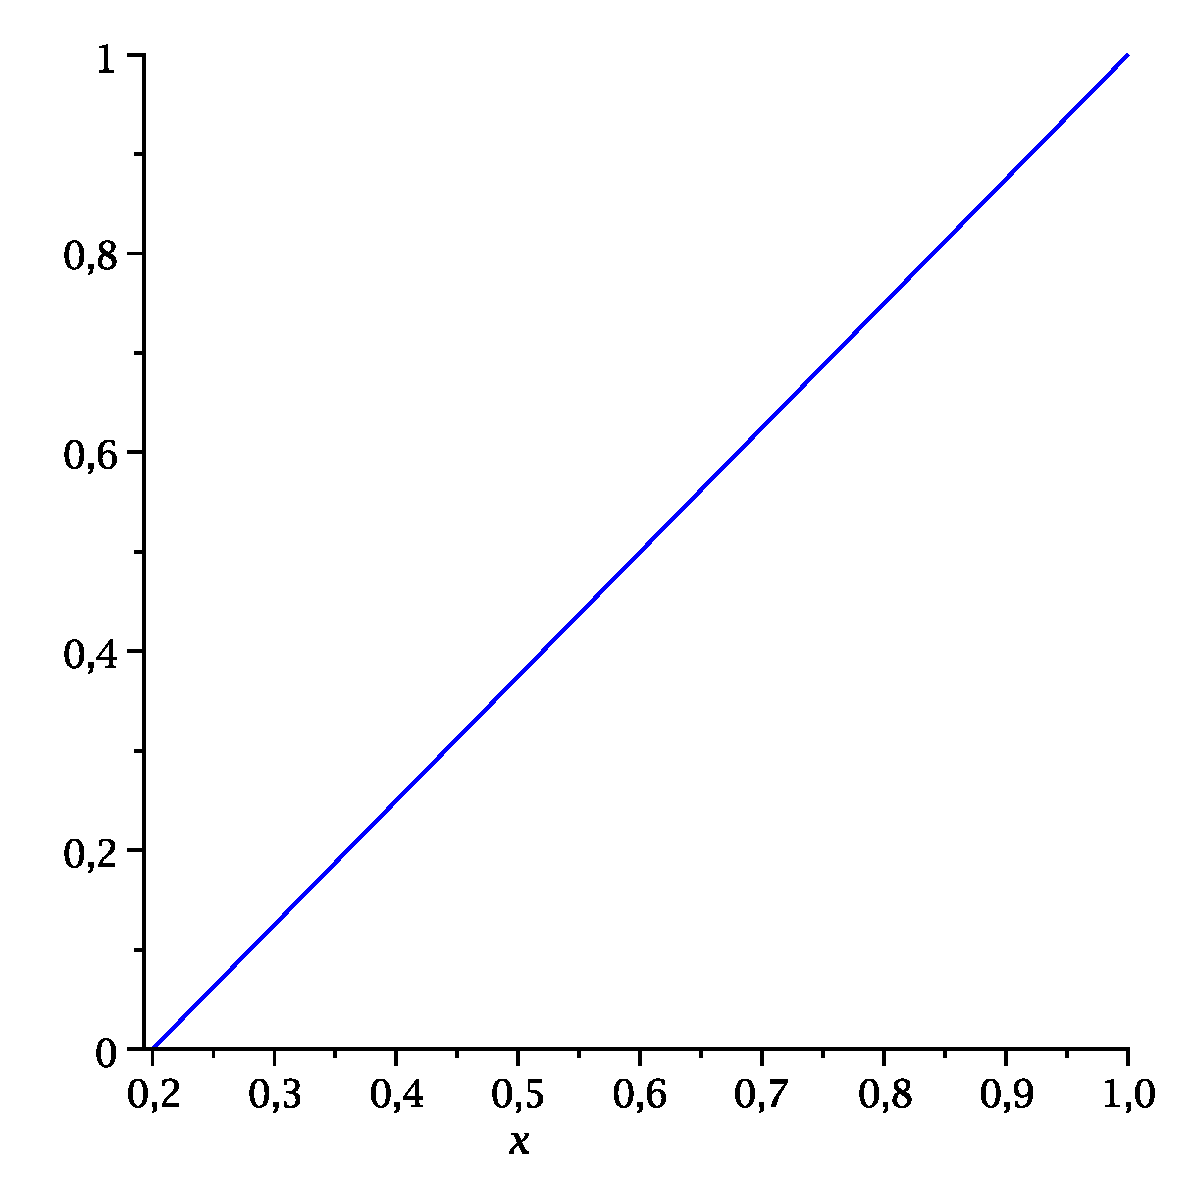
\includegraphics[scale=0.25]{soporte2.eps}
\end{array}
$$
}
%%%%
\frame
{
\frametitle{Ejemplo:}
\begin{eqnarray}
 P_1(x) & =& f(x_0)l_0(x) + f(x_1)l_1(x) = \nonumber\\
& &(0.4)e^{-2.8}\left(\frac{1-x}{0.8}\right) + 2e^{-6}\left(\frac{x-0.2}{0.8}\right)\nonumber\\
\Rightarrow P_1(x) &\approx& -0.02420815088x +0.02916565523\nonumber
\end{eqnarray}
\begin{center}
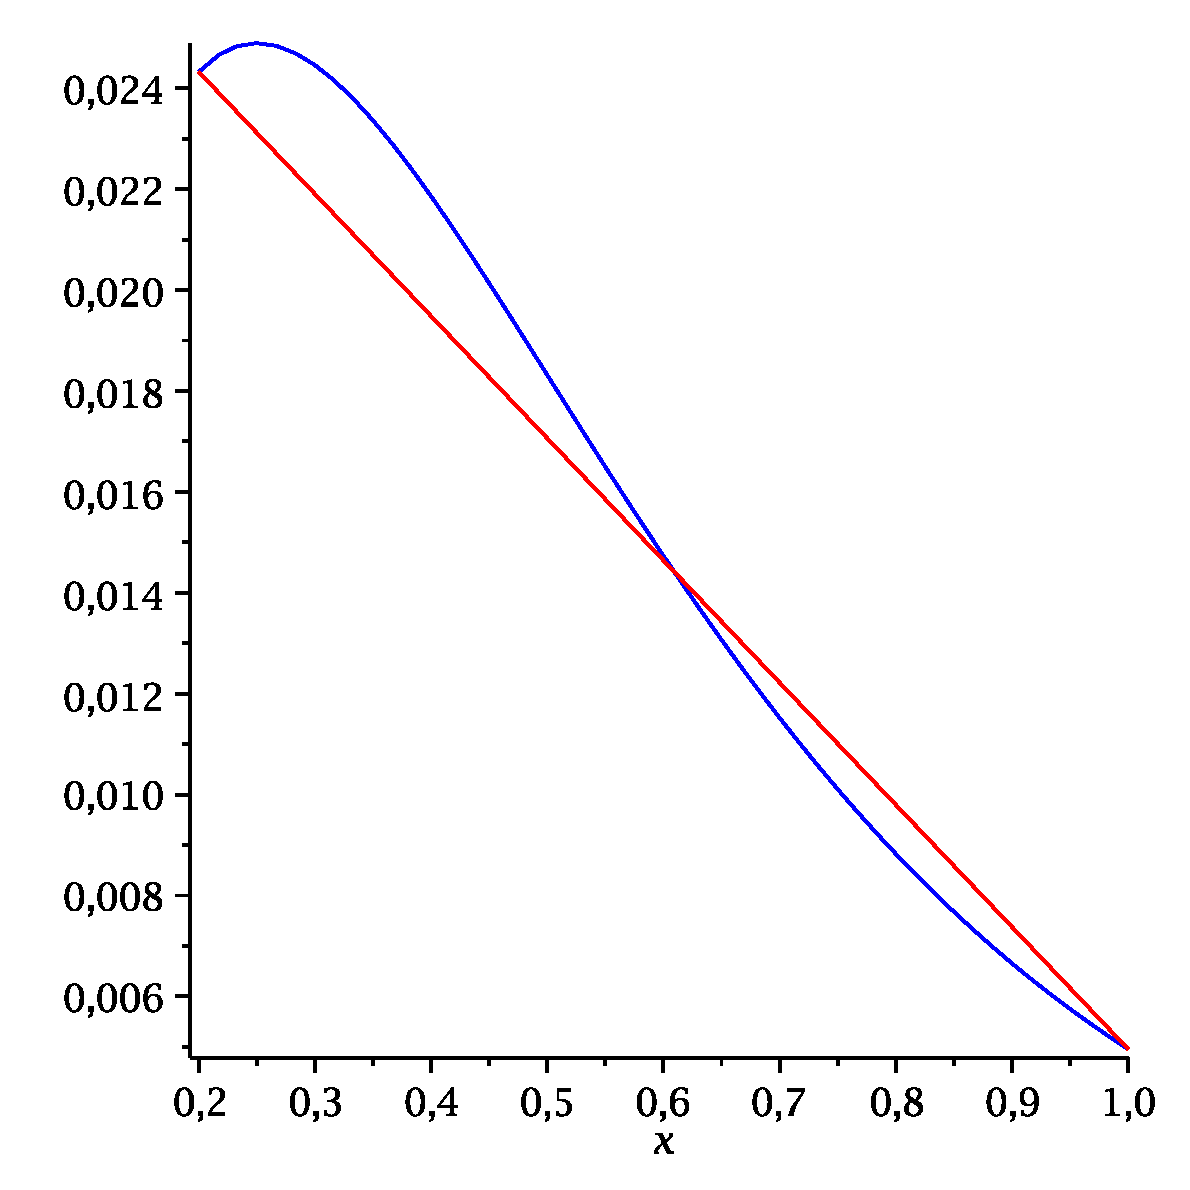
\includegraphics[scale=0.23]{approx.eps}
\end{center}
}
%%%
\frame
{
\frametitle{Expresi\'on del error}
Aplicamos la expresi\'on:
\begin{eqnarray}
 E(x)  =  f(x) - P_1(x) & = & \frac{f''(\xi_x)}{2!}\prod_{j=0}^1(x-x_j)\nonumber\\
E(x)  =  f(x) - P_1(x) & = & \frac{(-16+32\xi_x)e^{-(4\xi_x+2)}}{2!}(x-0.2)(x-1)\nonumber\\
E(x)  =  f(x) - P_1(x) & = & \frac{(-16+32\xi_x)e^{-(4\xi_x+2)}}{2}(x^2-1.2x+0.2)\nonumber
\end{eqnarray}
}
%%%%
\frame
{
\frametitle{Cota de error}
$$
\mid E(x)\mid  =  \mid f(x) - P_1(x)\mid  =  \frac{\displaystyle\max_{x\in[0.2,1]}\mid f''(x)\mid}{2!}\displaystyle\max_{x\in[0.2,1]}\left|\prod_{j=0}^1(x-x_j)\right|
$$
\uncover<2->{Obteniendo $g(x)=f''(x)=(-16+32x)e^{-(4x+2)}$, nos interesa $\max|f''(x)| $}
\uncover<3->{Dado que la funci\'on $g(x)$ es continua en $[0.2, 1]$, su mayor valor absoluto en $[0.2, 1]$ ser\'a el mayor de los siguientes:}
\begin{itemize}
 \item<4-> Valor de $|g(x)|$ en las abscisas de $[0.2, 1]$ para las que $g'(x) = 0$.
 \item<5-> Valor de $|g(0.2)|$.
 \item<6-> Valor de $|g(1)|$.
\end{itemize}
}
%%%%
\frame
{
\frametitle{Cota de error}
Valor de $|g(x)|$ en las abscisas para las que $g'(x) = 0$.
\uncover<2->{
$$
g(x) = (-16+32x)e^{-(4x+2)}\Rightarrow g'(x) = (96-128x)e^{-(4x+2)}
$$}
\uncover<3->{
$$
g'(x)=0 \Rightarrow (96-128x)e^{-(4x+2)}=0 \Rightarrow x^*=\frac{96}{128}=0.75
$$}
\uncover<4->{de donde $|g(0.75)|\approx0.0539$}
}
%%%%
\frame
{
\frametitle{Cota de error}
Valor de $g(x)$ en los extremos del intervalo $[ 0.2, 1]$.
\uncover<2->{
$$g(0.2) \approx -0.5838 = 0.5838$$
$$g(1) \approx 0.0397 = 0.0397$$}
\uncover<3->{\begin{center}
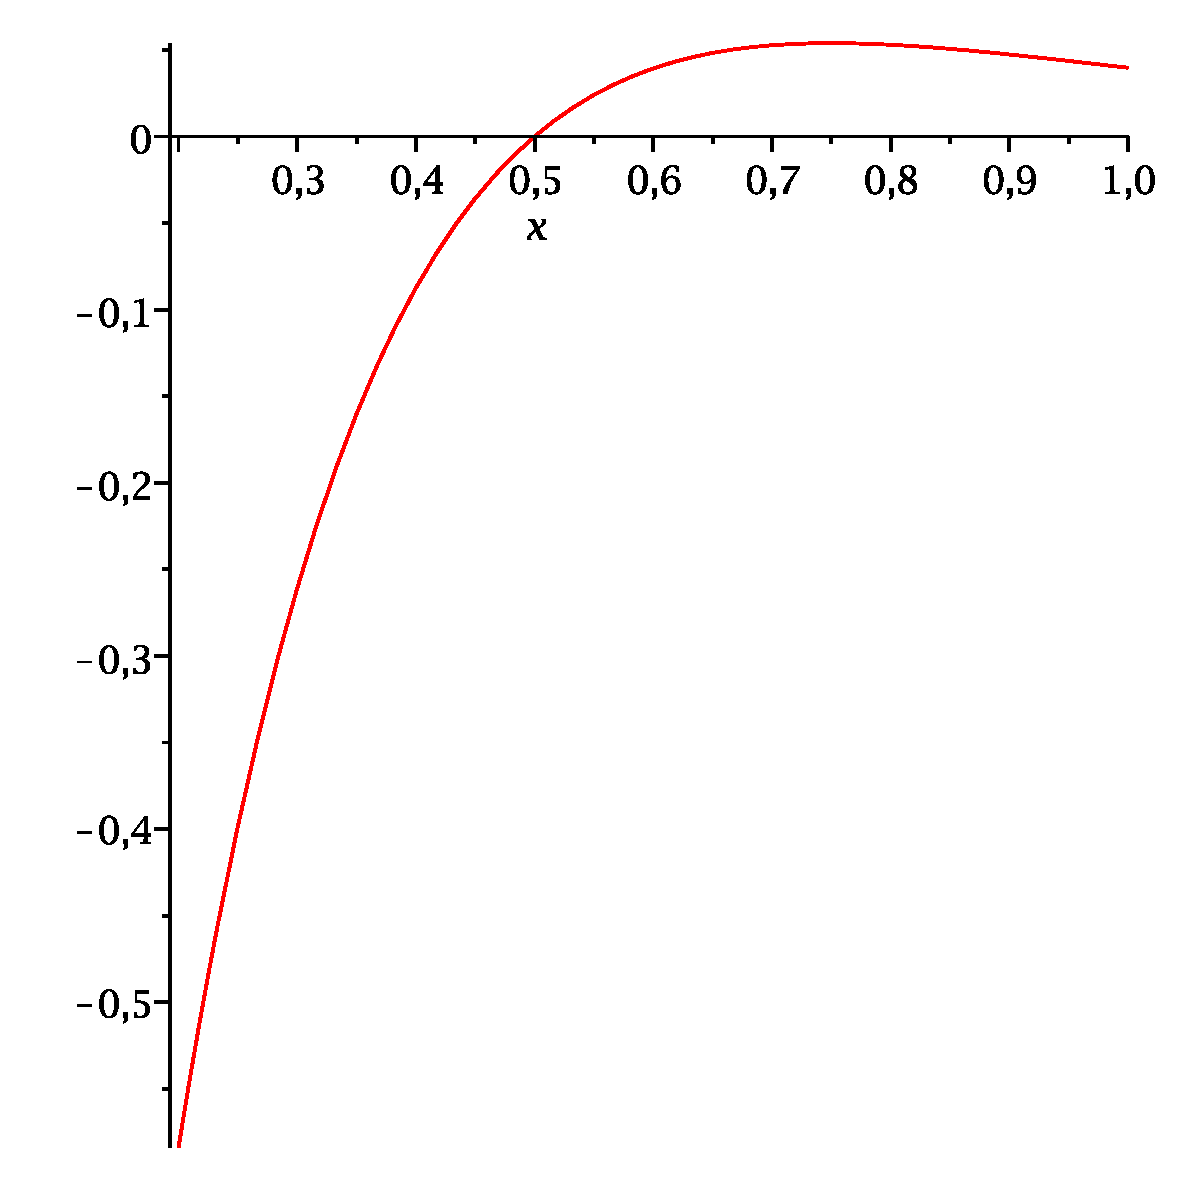
\includegraphics[scale=0.23]{gder.eps}
\end{center}}
}
%%%%
\frame
{
\frametitle{Cota de error}
Se busca ahora $\displaystyle\max_{x\in[0.2,1]}|(x-0.2)(x-1)|$
Llamamos $q(x)=(x - 0.2)(x - 1) = x^2 - 1.2x + 0.2$
\uncover<2->{$q(x)$ es un polinomio de segundo grado que se anula en los puntos $0.2$ y $1$, luego, necesariamente, tendr\'a alg\'un
extremo en el intervalo $[ 0.2, 1]$.}
\uncover<3->{\begin{center}
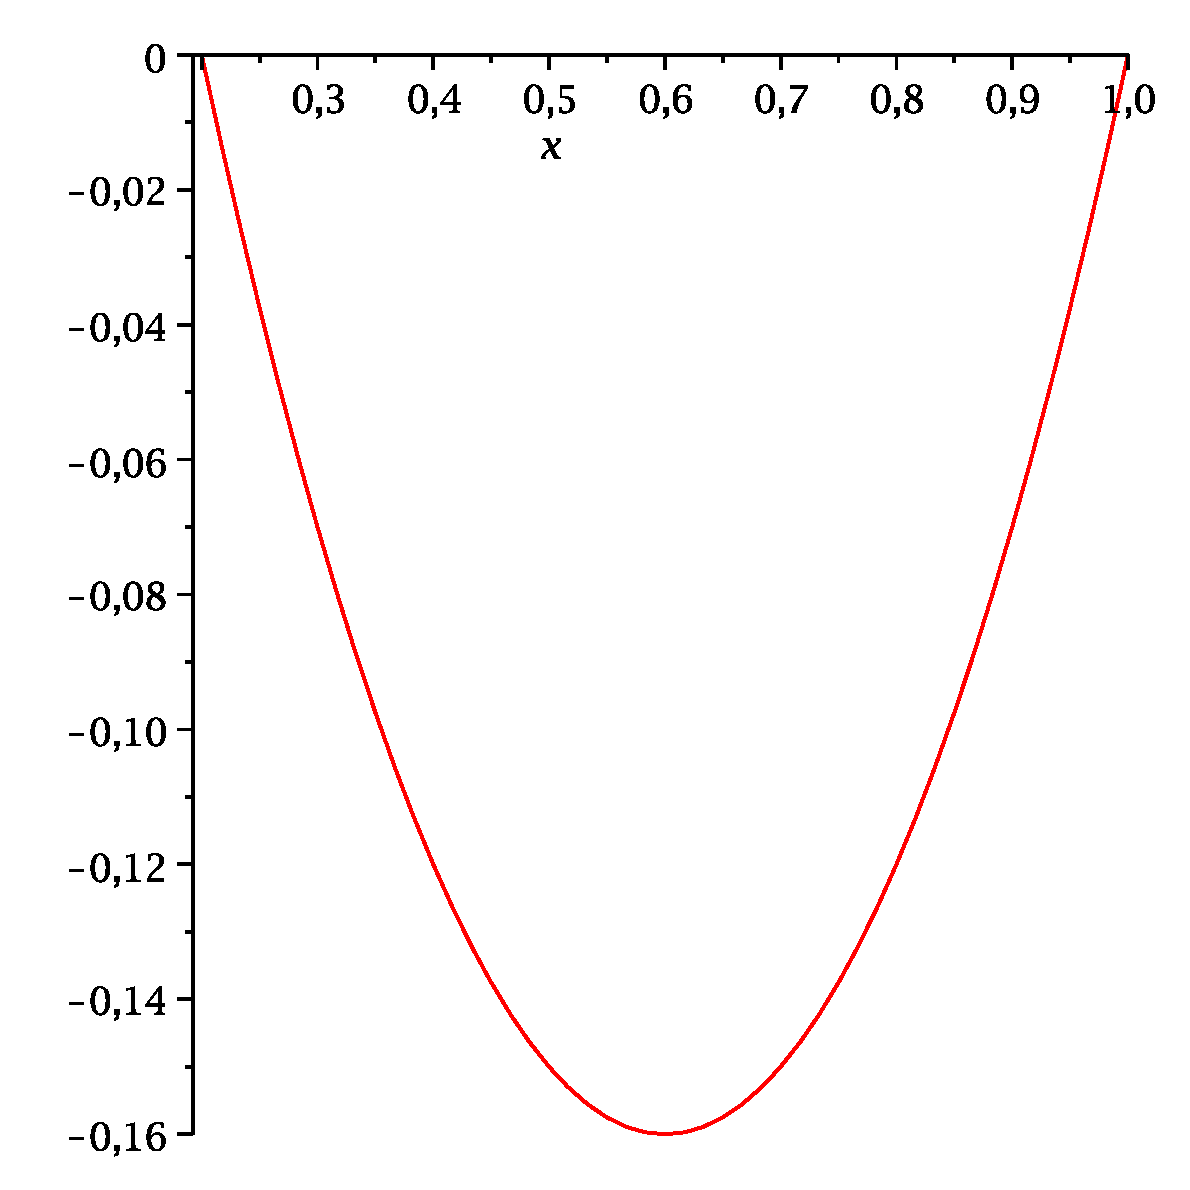
\includegraphics[scale=0.23]{parabola.eps}
\end{center}}
}
%%%
\frame
{
\frametitle{Cota de error}
El m\'aximo de $|q(x)|$ se alcanzar\'a en los puntos que se obtienen resolviendo la ecuaci\'on $q'(x) = 0$:
\uncover<2->{
$$
q'(x) = 0 = 2x - 1.2
$$}
\uncover<3->{
de donde se obtiene $x = 0.6$ como abscisa en la que se encuentra el m\'aximo de $q(x)$}
\uncover<4->{
$$q(0.6) = -0.16 \Rightarrow |q(0.6)| = 0.16$$}
}
%%%
\frame
{
\frametitle{Cota de error}
Teniendo en cuenta los resultados obtenidos, una cota de error vendr\'a dada por:
$$
|E(x)| = |f(x)-P_1(x)| \leq \frac{0.5838}{2}(0.16) = 0.046704
$$
}
%%%%
\frame
{
\frametitle{Cota de error}
La cota del error obtenida es una cota ``te\'orica''. Si se representa el valor absoluto del error exacto: $|E(x) | = | f(x) - P(x)|$ se obtiene la siguiente figura:
\uncover<2->{\begin{center}
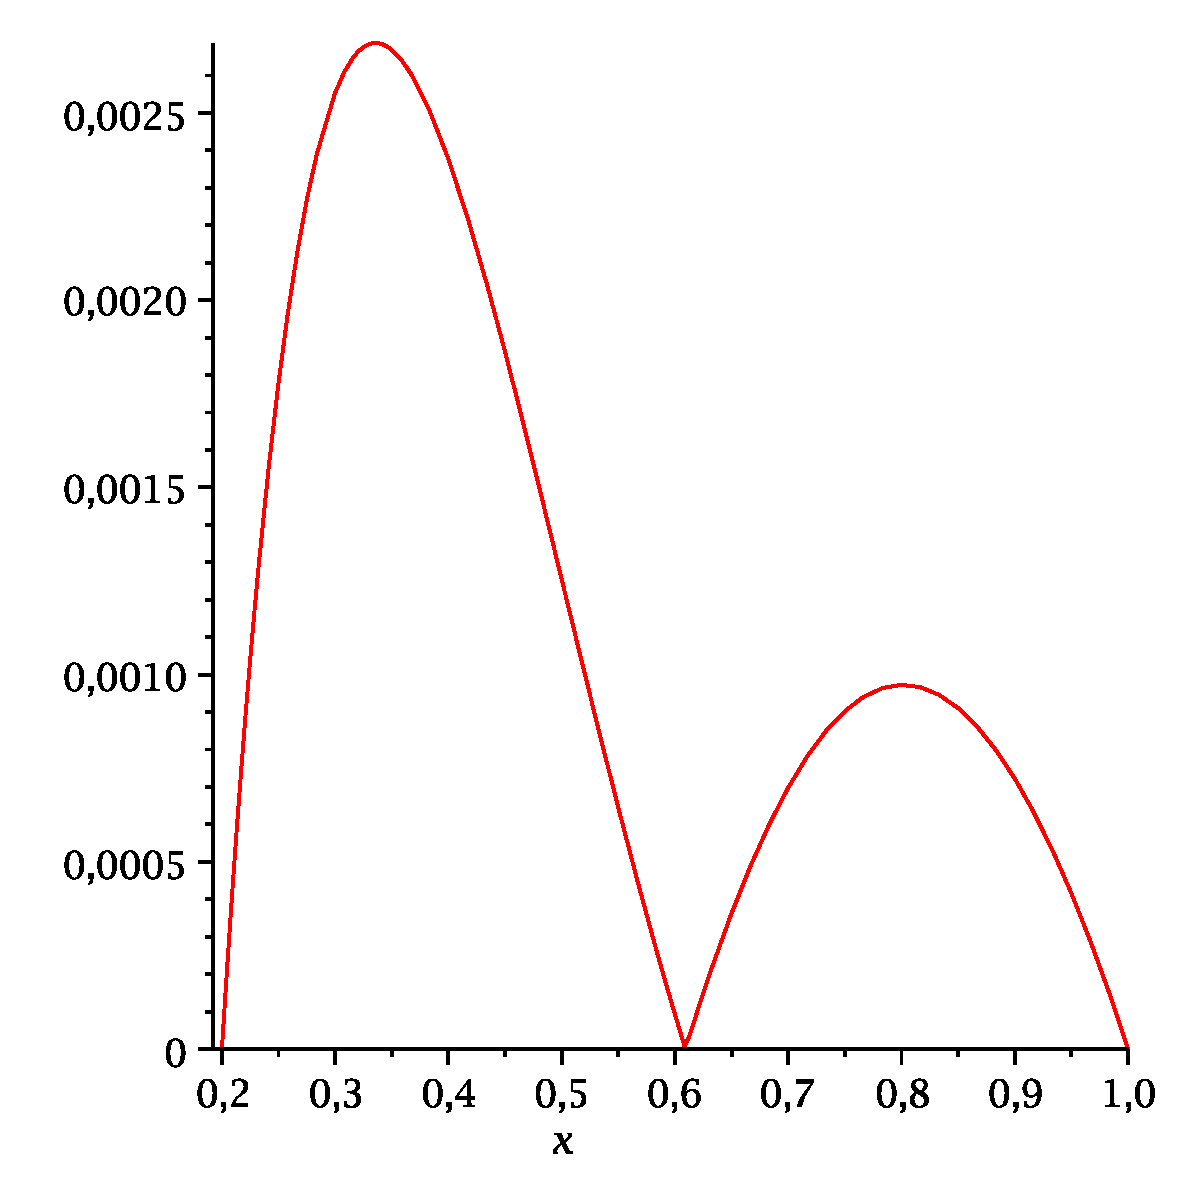
\includegraphics[scale=0.23]{error.eps}
\end{center}}
\uncover<3->{El error m\'aximo real que se comete es del orden de 0.0026, mucho menor que la cota te\'orica $0.046702$.}
}
%%%%
\frame
{
\frametitle{Desventajas:}
\begin{enumerate}
 \item<1-> El polinomio no viene expandido.
 \item<2-> La interpolaci\'on para otro valor de $x$ necesita la misma cantidad de c\'alculos adicionales, ya que no se pueden utilizar partes de la aplicaci\'on previa.
 \item<3-> La incorporaci\'on de un nuevo nodo obliga a rehacer todos los c\'alculos.
 \item<4-> La evaluaci\'on del error no es f\'acil.
\end{enumerate}
}
% %%%%%
\frame
{
\frametitle{Interpolaci\'on Iterada}
\begin{enumerate}
 \item<1-> A veces no es necesario obtener la forma expl\'icita del polinomio interpolador y basta con obtener su valor num\'erico 
 en un punto dado. 
 \item<2-> Adem\'as en este caso se desea poder aumentar el orden del polinomio interpolador a voluntad y parar 
 cuando el error sea suficientemente peque\~no. 
 \item<3-> Para estos prop\'ositos la interpolaci\'on iterada est\'a especialmente 
 indicado. 
\end{enumerate}
\uncover<4->{
\begin{center}
  \begin{block}{Definici\'on}
    Sea $f$ una funci\'on definida en $x_0,\ldots,x_n$ y supongamos $m_0,\ldots,m_k$ sean $k+1$ enteros distintos con 
$0 \leq m_i \leq n$ para cada $i=0,\ldots,k$. El polinomio de Lagrange de grado menor o igual a $k$ que coincide con 
$f$ en $x_{m_0},\ldots,x_{m_k}$ se denota $P_{m_0,\ldots,m_k}$.
\end{block}
\end{center}
}
}
%%%%
\frame
{
\frametitle{Ejemplo:}
Sea $f(x) = x^3$, $x_0 = 1, x_1 = 2, x_2 = 3, x_3 = 4, x_4 = 6$, calcule $P_{0,3,4}(x)$ y 
$P_{1,2,4}(x)$.
\uncover<2->{
  \footnotesize{
\begin{eqnarray}
\nonumber P_{0,3,4}(x) & = &  \dfrac{(x-4)(x-6)}{(1-4)(1-6)}1^3 + \dfrac{(x-1)(x-6)}{(4-1)(4-6)}4^3 + 
\dfrac{(x-1)(x-4)}{(6-1)(6-4)}6^3 =\\
\nonumber & = & 11x^2 - 34x + 24.
\end{eqnarray}}}
\uncover<3->{
  \footnotesize{
\begin{eqnarray}
\nonumber P_{1,2,4}(x) & = &  \dfrac{(x-3)(x-6)}{(2-3)(2-6)}2^3 + \dfrac{(x-2)(x-6)}{(3-2)(3-6)}3^3 + 
\dfrac{(x-2)(x-3)}{(6-2)(6-3)}6^3 =\\
\nonumber & = & 10x^2 - 27x + 18.
\end{eqnarray}}}
}
%%%%%
\frame
{
\frametitle{Interpolaci\'on Iterada}
\begin{block}{Teorema}
  Sea $f$ definida en $x_0,\ldots,x_k$ y sea $x_i,x_j$ dos n\'umeros distinto en este conjunto. Entonces el Polinomio de 
 Interpolaci\'on de Lagrange de grado menor o igual a $k$ que interpola a $f$ en $x_0,\ldots,x_k$ viene dado por la 
 siguiente relaci\'on:
 $$
 P(x) = \dfrac{(x-x_j)P_{0,\ldots,j-1,j+1,\ldots,k}(x) - (x-x_i)P_{0,\ldots,i-1,i+1,\ldots,k}(x)}{x_i - x_j}
 $$
 \end{block}
 \uncover<2->{
 \underline{Prueba:} Hay que probar que $P(x_s) = f(x_s), \forall s = 0,1,2,\ldots, k$.
 }
}
%%%%%
\frame
{
\frametitle{Interpolaci\'on Iterada}
 \noindent\textbf{Caso I}
 
 Sea $x_r \neq x_i$ y $x_r \neq x_j$ un nodo:
 \footnotesize{
 \begin{eqnarray}
  \nonumber P(x_r) & = & \dfrac{(x_r-x_j)P_{0,\ldots,j-1,j+1,\ldots,k}(x_r) - 
 (x_r-x_i)P_{0,\ldots,i-1,i+1,\ldots,k}(x_r)}{x_i - x_j}\\
 \nonumber & = & \dfrac{(x_r-x_j)f(x_r) -(x_r-x_i)f(x_r)}{x_i-x_j}\\
 \nonumber & = & \dfrac{-x_j+x_i}{x_i-x_j}f(x_r)\\
 \nonumber & = &  f(x_r)
 \end{eqnarray}}
}
%%%%
\frame{
 \frametitle{Interpolaci\'on Iterada} 
 \noindent\textbf{Caso II}
 
 Sea $x_r = x_i$
 \begin{eqnarray}
  \nonumber P(x_i) & = & \dfrac{(x_i-x_j)P_{0,\ldots,j-1,j+1,\ldots,k}(x_i) - 0}{x_i - x_j}\\
  \nonumber & = & \dfrac{x_i-x_j}{x_i-x_j}f(x_i)\\
  \nonumber & = &  f(x_i)
 \end{eqnarray}
 
 Es an\'alogo si $x_r = x_j$, por lo tanto $P(x)$ es el polinomio de Lagrange que coincide con $f$ en $x_0, x_1,\ldots , 
 x_k$ pues este es \'unico.
}
%%%%
\frame{
 \frametitle{M\'etodo de Neville} 
 Se desea aproximar $f(x^*)$ dada la siguiente tabla de valores para $f$:
\begin{center}
 \begin{tabular}{|c||c|c|c|c|}\hline
$x$ & $x_0$ & $x_1$ & $\cdots$ & $x_n$ \\\hline
$f(x)$ & $f(x_0)$ & $f(x_1)$ & $\cdots$ & $f(x_n)$\\\hline
\end{tabular}
\end{center}
Se genera la tabla de $f(x^*)$
$$
\begin{array}{ccccccc}
 x_0 & P_0 & & &  &  & \\ 
 x_1 & P_1 & P_{0,1} & &  &  & \\ 
 x_2 & P_2 & P_{1,2} & P_{0,1,2} &  &  & \\ 
 x_3 & P_3 & P_{2,3} & P_{1,2,3} & P_{0,1,2,3} &  & \\ 
 x_4 & P_4 & P_{3,4} & P_{2,3,4} & P_{1,2,3,4} & P_{0,1,2,3,4} & \\ 
 \vdots & \vdots & \vdots & \vdots & \vdots & \ddots & \\ 
 x_n & P_n & P_{n-1,n} & P_{n-2,n-1,n} & P_{n-3,n-2,n-1,n} & \cdots & P_{0,1,\ldots,n}
\end{array}
$$
}
%%%%%% 
\frame{
 \frametitle{M\'etodo de Neville} 
 \noindent\underline{Ejemplo:} Aproxime $f(2.5)$ dada la siguiente tabla
\begin{center}
\begin{tabular}{|c|c|c|}\hline
   & $x$   &  $f(x)$ \\ 
\hline
$x_0$ & $2.0$ & $0.5103757$\\ 
\hline
$x_1$ & $2.2$ & $0.5207843$\\ 
\hline
$x_2$ & $2.4$ & $0.5104147$\\ 
\hline
$x_3$ & $2.6$ & $0.4813306$\\ 
\hline
$x_4$ & $2.8$ & $0.4359160$\\ \hline
\end{tabular}
\end{center}
La tabla de Neville es
\footnotesize{
$$
\begin{array}{llllll}
   2.0 &  0.5103757 &            &               &                &              \\ 
   2.2 &  0.5207843 & \fbox{0.5363972}  &  \hookleftarrow P_{0,1}         &        &\\                          
   2.4 &  0.5104147 &  0.5052299 &  0.4974380750 &                &                   \\   
   2.6 &  0.4813306 &  0.4958726 &  0.4982119625 &  0.49808298125 &                  \\ 
   2.8 &  0.4359160 &  0.5040379 &  0.4979139625 &  0.49806296250 &  0.498070469531250
\end{array}
$$}
De donde $f(2.5) \approx 0.498070469531250$.
 }
 %%%%%%
 \frame{
 \frametitle{M\'etodo de Neville}
 Un ejemplo del c\'alculo la matriz anterior es:
\begin{eqnarray}
\nonumber P_{0,1} & = & \dfrac{(x-x_0)P_1 - (x-x_1)P_0}{x_1-x_0}\\ 
\nonumber & = & \dfrac{(2.5 - 2.0)0.5207843- (2.5 - 2.2)0.5103757}{2.2 - 2.0}\\ 
\nonumber & = & 0.5363972
\end{eqnarray}
}
%%%%%
\frame{
 \frametitle{M\'etodo de Neville}
 \begin{block}{Notaci\'on}
  Se denota por $Q_{ij}$ el polinomio interpolante de Lagrange de grado $j$ que pasa por 
los $j + 1$ nodos siguientes:
$$
x_{i-j},x_{i-j+1},\ldots,x_{i-1},x_i
$$
es decir
$$
Q_{ij} = P_{i-j,i-j+1,\ldots,i-1,i}(x)
$$
\end{block}
\uncover<2->{
Ahora usando el m\'etodo de Neville 
\small{
\begin{eqnarray}
\nonumber Q_{ij} & = & \dfrac{(x-x_i)P_{i-j,i-j+1,\ldots,i-1}(x) - (x-x_{i-j})P_{i-j+1,\ldots,i-1,i}(x)}{x_{i-j}-x_i}\\ 
\nonumber & = & \dfrac{(x-x_{i-j})P_{i-j+1,\ldots,i-1,i}(x) - (x-x_i)P_{i-j,i-j+1,\ldots,i-1}(x)}{x_i-x_{i-j}}\\ 
\nonumber & = & \dfrac{(x-x_{i-j})Q_{i,j-1} - (x-x_i)Q_{i-1,j-1}}{x_i-x_{i-j}}
\end{eqnarray}
}}}
%%%%
\frame{
 \frametitle{M\'etodo de Neville}
Con esta nueva notaci\'on, la tabla de Neville se puede escribir como:
$$
\begin{array}{ccccccc}
 x_0 & Q_{00} & & &  &  & \\ 
 x_1 & Q_{10} & Q_{11} & &  &  & \\ 
 x_2 & Q_{20} & Q_{21} & Q_{22} &  &  & \\ 
 x_3 & Q_{30} & Q_{31} & Q_{32} & Q_{33} &  & \\ 
 \vdots & \vdots & \vdots & \vdots & \vdots & \ddots & \\ 
 x_n & Q_{n0} & Q_{n1} & Q_{n2} & Q_{n3} & \cdots & Q_{nn}
\end{array}
$$
}
%%%%%
\begin{frame}
  \frametitle{M\'etodo de Neville}
  \begin{algorithm}[H]
    \SetKwInOut{Input}{input}
    \SetKwInOut{Output}{output}
    \caption{Algoritmo para calcular la tabla de Neville y aproximar $f(x^*)\approx P_n(x^*)$.}
    \Input{Los nodos $x_0,x_1,\ldots,x_n$. Sus im\'agenes $f(x_0),f(x_1),\ldots,f(x_n)$ como primera columna de $Q$}
    \Output{La tabla o matriz $Q$, donde $f(x^*) \approx Q_{nn}$.}
    %\BlankLine
    \For{$i\leftarrow 1$ \KwTo $n$}
    {
       \For{$j\leftarrow 1$ \KwTo $i$}
       {
         $Q_{ij} \leftarrow \dfrac{(x-x_{i-j})Q_{i,j-1} - (x-x_i)Q_{i-1,j-1}}{x_i-x_{i-j}}$
       }
    }
    Salida $Q_{nn}$
    \label{neville}
   \end{algorithm}
\end{frame}
%%%%%
\frame{
 \frametitle{M\'etodo de Aitken} 
 Existe el m\'etodo de Aitken, que es similar al m\'etodo de Neville, y que se genera de manera similar.
$$
\begin{array}{ccccccc}
 x_0 & P_0 & & &  &  & \\ 
 x_1 & P_1 & P_{0,1} & &  &  & \\ 
 x_2 & P_2 & P_{0,2} & P_{0,1,2} &  &  & \\ 
 x_3 & P_3 & P_{0,3} & P_{0,1,3} & P_{0,1,2,3} &  & \\ 
 x_4 & P_4 & P_{0,4} & P_{0,1,4} & P_{0,1,2,4} & P_{0,1,2,3,4} & \\ 
 \vdots & \vdots & \vdots & \vdots & \vdots & \ddots & \\ 
 x_n & P_n & P_{0,n} & P_{0,1,n} & P_{0,1,2,n} & \cdots & P_{0,1,\ldots,n}
\end{array}
$$
}
%%%%%
\begin{frame}
  \frametitle{M\'etodo de Interpolaci\'on Inversa}
  \begin{itemize}
    \item Sea $f \in C^1[a,b]$, $f'(x) \neq 0$ en $[a,b]$ y que $f$ posee un cero $p$ en $[a,b]$.
    \item<2-> Sea $x_0,\ldots,x_n$ $n+1$ n\'umeros distintos en $[a,b]$ con $f(x_k)=y_k$ para cada $k=0,\ldots,n$.
    \item<3-> Si se quiere aproximar $p$, se construye el 
    polinomio interpolante de grado $n$ en los nodos $y_0,\ldots,y_n$ para $f^{-1}$.
    \item<4-> Puesto que $y_k=f(x_k)$ y $0=f(p)$, se 
    deduce que $f^{-1}(y_k)=x_k$ y $p=f^{-1}(0)$.
    \item<5-> Se da el nombre de interpolaci\'on iterada inversa al uso de la
    interpolaci\'on para aproximar $f^{-1}(0)$.
  \end{itemize}  
\end{frame}
%%%%%
\frame{
 \frametitle{Ejercicios:}
 \begin{enumerate}
  \item Aproximar $\sqrt{3}$ usando el m\'etodo de Neville y Aitken en la funci\'on $f(x)=3^x$ para los valores 
$x_0=-2$, $x_1=-1$, $x_2=0$, $x_3=1$, $x_4=2$.
 \item Realizar el algoritmo del m\'etodo de Aitken.
 \item Use la interpolaci\'on iterada inversa para obtener una aproximaci\'on a la soluci\'on de $x-e^{-x}=0$, por 
medio de los datos:
$$
\begin{array}{c|c|c|c|c}
 x & 0.3 & 0.4 & 0.5 & 0.6 \\ \hline
e^{-x} & 0.740818 & 0.670320 & 0.606531 & 0.548812
\end{array}
$$
\item Construya un algoritmo que sirva para obtener la interpolaci\'on iterada inversa.
\end{enumerate}
}
%%%%
\subsection{Newton}
\frame{
  \frametitle{F\'ormula de Newton del Polinomio de Interpolaci\'on}
  \begin{itemize}
    \item<1-> En ocasiones es \'util considerar varios polinomios aproximantes $P_1(x),P_2(x),\ldots,P_n(x)$ y, despu\'es, elegir el m\'as adecuado a las necesidades.
    \item<2-> Uno de los inconvenientes de los polinomios interpoladores de Lagrange es que no hay relaci\'on entre la construcci\'on de $P_{n-1}(x)$ y la de $P_n(x)$; cada polinomio debe construirse individualmente y se requieren muchas operaciones para calcular polinomios de grado elevado.
    \end{itemize}
}
%%%%
\frame{
  \frametitle{F\'ormula de Newton del Polinomio de Interpolaci\'on}
  \begin{itemize}
    \item<1-> Dados $n+1$ puntos $(x_0,y_0),(x_1, y_1),\ldots,(x_n, y_n)$ con $x_0,x_1,\ldots,x_n$ n\'umeros distintos y $y_k=f(x_k)$, $k=0,1,\ldots,n$ para alguna funci\'on $f$ definida en un intervalo $[a,b]$ que contiene a los nodos. 
    \item<2-> El polinomio $P(x)$ de grado menor o igual a $n$ que interpola a $f$ en los datos dados, puede expresarse en la forma:
    \footnotesize{
    $$
    P_n(x) = a_0 + a_1 (x - x_0 ) + a_2 (x - x_0 )( x - x_1 ) + \cdots + a_n ( x - x_0 )( x - x_1 )\cdots( x - x_{n-1})
    $$
    }
    \normalsize
    es decir:
    $$
    p_n(x) = a_0 + \sum_{j=1}^na_j\prod_{k=0}^{j-1}(x-x_k)
    $$
    para ciertas constantes $a_0, a_1,\ldots, a_n$    
    \end{itemize}
}
%%%%%
\frame{
 \frametitle{F\'ormula de Newton del Polinomio de Interpolaci\'on}
 \begin{itemize}
  \item<1-> Algunas propiedades de esta forma de representar el 
  polinomio de interpolaci\'on permite la construcci\'on de un polinomio 
  de interpolaci\'on de grado $k$ a partir del de grado menor $k - 1$.
  \item<2-> Sea $q_k(x)$ la suma de los primeros $k + 1$ t\'erminos de $p_n(x)$, es decir
  \footnotesize{
  $$
  q_k(x) =  a_0 + a_1 (x - x_0 )+a_2 (x - x_0 )(x - x_1 ) + \cdots + a_k(x - x_0 )(x - x_1 ) \cdots (x - x_{k-1} )
  $$}
  \item<3-> Entonces los t\'erminos restantes de $p_n(x)$ tienen como factor com\'un el producto
  $$
  (x - x_0 )(x - x_1 ) \cdots (x - x_k)
  $$
  \end{itemize}
}  
%%%%%%
\frame{
  \frametitle{F\'ormula de Newton del Polinomio de Interpolaci\'on}
  \begin{itemize}
  \item As\'i que
  $$
  p_n(x) = q_k(x) + (x - x_0 )(x - x_1 ) \cdots (x - x_k)r(x)
  $$
  donde $r(x)$ es un polinomio de grado $\leq n - (k + 1)$.
  \item<2-> Adem\'as $q_k(x)$ interpola $f(x)$ en los puntos $x_0 , x_1 , 
  \ldots , x_k$ , pues
  \begin{eqnarray}
  \nonumber q_k(x_j) & = & p_n(x_j) - (x_j - x_0 )(x_j - x_1 ) \cdots (x_j - x_k)r(x_j)\\ 
  \nonumber & = & p_n(x_j) \quad \mbox{ si } 0 \leq j \leq k\\ 
  \nonumber & = & f(x_j)
  \end{eqnarray}
\end{itemize}  
}
%%%%%
\frame{
  \frametitle{F\'ormula de Newton del Polinomio de Interpolaci\'on}
  \begin{itemize}
  \item Entonces $q_k(x)$ es el \'unico polinomio de interpolaci\'on $p_k(x)$ para $f(x)$ en $x_0 , x_1 , \ldots , x_k$, y
  se puede escribir
  $$
  p_{k+1}(x) = q_k(x) + (x - x_0 )(x - x_1 ) \cdots (x - x_k)r(x)
  $$
  \item<2-> y con $k = n - 1$, se obtiene
  $$
  p_n(x) = p_{n-1}(x) + a_n (x - x_0 )(x -x_1 ) \cdots (x - x_{n-1} )
  $$
  \item<3-> Entonces, el polinomio de interpolaci\'on $p_n(x)$ puede construirse paso a paso construyendo la sucesi\'on de 
  polinomios de interpolaci\'on $p_0 (x), p_1 (x),\ldots, p_n (x)$, donde $p_k (x)$ se construye de $p_{k-1} (x)$ 
  agregando el siguiente t\'ermino en la forma de Newton , el cual es
  $$
  a_k (x - x_0 )(x - x_1 ) \cdots (x - x_{k-1} )
  $$  
\end{itemize}
}  
%%%%
\frame{
\frametitle{Polinomio Interpolador de Newton}
Los polinomios interpoladores de Newton se calculan mediante un esquema recursivo
\begin{block}{}
  \footnotesize{
$$
\begin{array}{lcl}
  P_0(x) & = & a_0\\ 
P_1(x) & = & a_0+a_1(x-x_0)\\ 
P_2(x) & = & a_0+a_1(x-x_0)+a_2(x-x_0)(x-x_1)\\ 
P_3(x) & = & a_0+a_1(x-x_0)+a_2(x-x_0)(x-x_1)+a_3(x-x_0)(x-x_1)(x-x_2)\\ 
\vdots & \vdots & \vdots\\ 
P_n(x) &  & a_0+a_1(x-x_0)+a_2(x-x_0)(x-x_1)+a_3(x-x_0)(x-x_1)(x-x_2)\\ 
       &  & +a_4(x-x_0)(x-x_1)(x-x_2)(x-x_3)+\cdots\\ 
       &  & +a_n(x-x_0)(x-x_1)(x-x_2)\cdots(x-x_{n-2})(x-x_{n-1})
\end{array}
$$}
\end{block}
}
%%%%
\frame{
\frametitle{Polinomio Interpolador de Newton}
\begin{itemize}
  \item<1-> Las $n + 1$ ecuaciones que surgen al evaluar $x_i$ se pueden expresar matricialmente como
\small{
  $$
\left[\begin{array}{cccc}
1 & 0 & \cdots & 0\\ 
1 & (x_1-x_0) & \cdots & 0\\ 
\vdots & \vdots & & \\ 
1 & (x_n-x_0) & (x_n-x_0)(x_n-x_1) & \cdots(x_n-x_0)
\end{array}\right]\left[\begin{array}{c}a_0\\a_1\\\vdots\\a_n\end{array}\right]=\left[\begin{array}{c}f(x_0)\\f(x_1)\\\vdots\\f(x_n)\end{array}\right]
$$}
\item<2-> La matriz del sistema es triangular inferior.
\item<3-> $O(n^2)$ operaciones necesarias para resolver el sistema.
\end{itemize}
}
%%%%%%
\frame{
\frametitle{Polinomio Interpolador de Newton}
C\'alculo de los coeficientes $a_0, a_1, \ldots a_n$.
\begin{itemize}
\item Se puede observar que cada coeficiente $a_k$ es el coeficiente principal del polinomio $p_k(x)$ que interpola a $f$ 
en los puntos $x_0 , x_1 , \ldots , x_k$.
\item<2-> Adem\'as este coeficiente depende de los puntos y valores de $f(x)$ en estos 
puntos
\begin{eqnarray}
\nonumber f(x_0) & = & p_0(x_0) = a_0\\ 
\uncover<3->{\nonumber f(x_1) & = & p_1(x_1) = f(x_0) + a_1(x_1-x_0)}\\ 
\uncover<4->{\nonumber f(x_2) & = & p_2(x_2) = f(x_0) + a_1(x_2-x_0) + a_2(x_2-x_1)\\ 
\nonumber & \Rightarrow & a_1 = \dfrac{f(x_1)-f(x_0)}{x_1-x_0}}
\end{eqnarray}
\end{itemize}
}
%%%%%%
\frame{
\frametitle{Polinomio Interpolador de Newton}
\scriptsize{  
\begin{eqnarray}
\nonumber f(x_2) & = & p_2(x_2) = p_1(x_2) + a_2(x_2-x_0)(x_2-x_1)\\ 
\uncover<2->{\nonumber & \Rightarrow & a_2 = \dfrac{f(x_2)-p_1(x_2)}{(x_2-x_0)(x_2-x_1)} = \dfrac{f(x_2)-f(x_0) - 
a_1(x_2-x_0)}{(x_2-x_0)(x_2-x_1)}}\\ 
\uncover<3->{\nonumber & \Rightarrow & a_2 = \dfrac{f(x_2)-f(x_0)}{(x_2-x_0)(x_2-x_1)} - 
\dfrac{\frac{f(x_1)-f(x_0)}{x_1-x_0}(x_2-x_0)}{(x_2-x_0)(x_2-x_1)}}\\ 
\uncover<4->{\nonumber & \Rightarrow & a_2 =  \dfrac{f(x_2)-f(x_0)}{(x_2-x_0)(x_2-x_1)} -  
\dfrac{f(x_1)-f(x_0)}{(x_1-x_0)(x_2-x_1)}}\\ 
\uncover<5->{\nonumber  &\Rightarrow & \frac{x_1f(x_2) - x_1f(x_0) - x_0f(x_2) + x_0f(x_0) - x_2f(x_1) + x_0f(x_1) 
+ x_2f(x_0) - x_0f(x_0)}{(x_1 - x_0)(x_2 - x_0)(x_2 - x_1)}}\\ 
\uncover<6->{\nonumber &\Rightarrow& a_2 = \dfrac{f(x_2)(x_1 - x_0) - f(x_1)(x_1 - x_0) - f(x_1)(x_2 - x_1) + f(x_0)(x_2 - 
x_1)}{(x_1 - x_0)(x_2 - x_0)(x_2 - x_1)}}\\ 
\uncover<7->{\nonumber &\Rightarrow& a_2 = \left(\dfrac{(x_1 - x_0)(f(x_2) - f(x_1))}{(x_1 - x_0)(x_2 - x_1)} - \dfrac{(x_2 - x_1
)(f(x_1) - f(x_0))}{(x_1 - x_0)(x_2 - x_1)}\right)\dfrac{1}{x_2 - x_0}}\\ 
\uncover<8->{\nonumber &\Rightarrow& a_2 = \dfrac{\dfrac{f(x_2) - f(x_1)}{x_2 - x_1} - \dfrac{f(x_1) - f(x_0)}{x_1 - x_0}}{x_2 - x_0}}
\end{eqnarray}}
\normalsize
\uncover<9->{El numerador es una diferencia de cocientes de diferencias, a cada uno de estos cocientes, se les llama diferencias divididas}
}
%%%%%
\frame{
\frametitle{Polinomio Interpolador de Newton}
\begin{block}{Definici\'on}
  Dados $n+1$ puntos $(x_0,f(x_0)),(x_1, f(x_1)),\ldots,(x_n,f(x_n))$ con $x_0, x_1, \ldots, x_n$ n\'umeros distintos y $f$ alguna
  funci\'on definida sobre ella, se define:
  \begin{enumerate}
   \item<2-> \textbf{La diferencia dividida cero de $f$ con respecto a $x_k$ es}:
   $$
   \mathcal{F}[x_k] = f(x_k), \quad \forall k=0,1,\ldots,n
   $$
   por lo tanto en el polinomio interpolante se tiene que $a_0=\mathcal{F}[x_0]$
   \item<3-> \textbf{La diferencia dividida uno de $f$ respecto a $x_k$ y $x_{k+1}$ es}:
 $$
 \mathcal{F}[x_k.x_{k+1}] = \dfrac{\mathcal{F}[x_{k+1}] - \mathcal{F}[x_k]}{x_{k+1} - x_k}, \quad \forall k=0,1,\ldots,n-1 
 $$
 las diferencias divididas uno dependen de las diferencias divididas cero, dado que existen $n+1$ diferencias divididas cero, solo hay $n$ diferencias divididas uno. Se tiene que $a_1 = \mathcal{F}[x_0,x_1] = \dfrac{\mathcal{F}[x_1] - \mathcal{F}[x_0]}{x_1 - x_0}$
  \end{enumerate}
\end{block}
}
%%%%%
\frame{
\frametitle{Polinomio Interpolador de Newton}
\begin{block}{Definici\'on}
  \begin{enumerate}
    \setcounter{enumi}{2}
    \item \textbf{La diferencia dividida dos de $f$ con respecto a $x_k$, $x_{k+1}$ y $x_{k+2}$ es}:
  $$
  \mathcal{F}[x_k.x_{k+1},x_{k+2}] = \dfrac{\mathcal{F}[x_{k+1},x_{k+2}] - \mathcal{F}[x_k,x_{k+1}]}{x_{k+2} - x_k}, \quad \forall k=0,1,\ldots,n-2
  $$
  las diferencias divididas dos dependen de las diferencias divididas uno, dado que existen $n$ diferencias divididas uno, solo hay $n-1$ diferencias divididas dos.
 Obs\'ervese que en el polinomio 
 $$
 a_2 = \mathcal{F}[x_0,x_1,x_2] = \dfrac{\mathcal{F}[x_1,x_2] - \mathcal{F}[x_0,x_1]}{x_2 - x_0}
 $$   
\end{enumerate}
\end{block}
}
%%%%
\frame{
\frametitle{Polinomio Interpolador de Newton}
\begin{block}{Definici\'on}
  \begin{enumerate}
    \setcounter{enumi}{3}
    \item En general conocidas las $n-(i-1)+1=n-i+2$ diferencias divididas $i-1$ de $f$ con respecto a $x_k, x_{k+1}, \ldots,
    x_{k+i-1}$, $\mathcal{F}[x_k, x_{k+1}, \ldots, x_{k+i-1}]$, $k=0,1,\ldots, n-(i-1)$, se definen las $n-i+1$ \textbf{diferencias divididas $i$ de $f$ con respecto a $x_k, x_{k+1},\ldots, x_{k+i}$}, as\'i
    $$
    \mathcal{F}[x_k.x_{k+1},\ldots,x_{k+i}] = \dfrac{\mathcal{F}[x_{k+1},x_{k+2},\ldots,x_{k+i}] - \mathcal{F}[x_k,x_{k+1},\ldots,x_{k+i-1}]}{x_{k+i} - x_k}    
    $$
    $$
    \forall k=0,1,\ldots,n-i
    $$
  \end{enumerate}
\end{block}
}
%%%%
%%%%%
\frame
{
\frametitle{Polinomio Interpolador de Newton}
Con esta notaci\'on de diferencia dividida se tiene que $a_i=\mathcal{F}[x_0,x_1,\ldots,x_i]$, $i=0,1,\ldots,n$ y as\'i el polinomio interpolante toma la siguiente forma:
\small
\begin{block}{}
$$
P_n(x) = \mathcal{F}[x_0] + \mathcal{F}[x_0,x_1](x - x_0 ) +  \cdots + \mathcal{F}[x_0,x_1,\ldots,x_n](x - x_0 )\cdots(x - x_{n-1})
$$
\end{block}
}
%%%
\frame
{
\frametitle{Polinomio Interpolador de Newton}
\textbf{?`C\'omo organizar el c\'alculo de la tabla de diferencias divididas?}\\[15pt]
\uncover<2->{El c\'alculo de las diferencias divididas para cuatro puntos se ordenar\'ia como sigue:
\begin{block}{}
$$
\begin{array}{llll}
 x_0 \rightarrow y_0=\mathcal{F}[x_0] & & &\\
 x_1 \rightarrow y_1=\mathcal{F}[x_1] & \mathcal{F}[x_0,x_1] & &\\
 x_2 \rightarrow y_2=\mathcal{F}[x_2] & \mathcal{F}[x_1,x_2] & \mathcal{F}[x_0,x_1,x_2] &\\
 x_3 \rightarrow y_3=\mathcal{F}[x_3] & \mathcal{F}[x_2,x_3] & \mathcal{F}[x_1,x_2,x_3] & \mathcal{F}[x_0,x_1,x_2,x_3]\\
\end{array}
$$
\end{block}
}
}
%%%%
\frame
{
\frametitle{Polinomio Interpolador de Newton}
\begin{itemize}
  \item Esta forma del polinomio interpolante de Newton se conoce como F\'ormula de Diferencias Divididas Progresivas Interpolante de
  Newton, y se usa en los c\'alculos num\'ericos cuando se interpola en un punto $x$ que est\'a m\'as cerca de $x_0$ que de $x_n$.
  \item<2-> Si el punto $x$ en el cual vamos a interpolar est\'a mas cerca de $x_n$ que de $x_0$ se usa la F\'ormula de Diferencias Divididas Regresivas Interpolante de Newton:
  \scriptsize{
  $$
   p_n(x) = f[x_n] + f[x_{n-1},x_n] (x - x_n) +  + \cdots + f[x_n,x_{n-1},\ldots,x_0](x
  - x_n )(x - x_{n-1}) \cdots (x - x_1)
  $$}
\end{itemize}
}
%%%%
\frame
{
\frametitle{Ejemplo:}
Obtener el polinomio interpolador para la funci\'on $f(x) = \sin(x)$ sobre el soporte formado por los puntos:
$$
x=\left\{0,\frac{\pi}{4},\frac{\pi}{2}\right\}
$$
\uncover<2->{
Tabla de Diferencias Divididas
\begin{block}{}
$$
\begin{array}{ccccc}
 0 &  \rightarrow & 0 & &\\
 \frac{\pi}{4} & \rightarrow & \dfrac{1}{\sqrt{2}} & \dfrac{2\sqrt{2}}{\pi} &\\
 \frac{\pi}{2} & \rightarrow & 1 & \dfrac{2(2-\sqrt{2})}{\pi} & \dfrac{8(1-\sqrt{2})}{\pi^2}\\
\end{array}
$$}
\end{block}
}
%%%%
\frame
{
\frametitle{Ejemplo:}
Formando el polinomio interpolante de Newton
\begin{block}{}
$$
P_2(x) = \mathcal{F}[x_0] + \mathcal{F}[x_0,x_1](x - x_0) + \mathcal{F}[x_0,x_1,x_2](x - x_0)(x-x_1)
$$
$$
= 0 + \frac{2\sqrt{2}}{\pi}(x-0) + \frac{8(1-\sqrt{2})}{\pi^2}(x-0)(x-\frac{\pi}{4}
)$$
\end{block}
}
% %%%%
\frame
{
\frametitle{Ejemplo:}
$$
\begin{array}{cc}
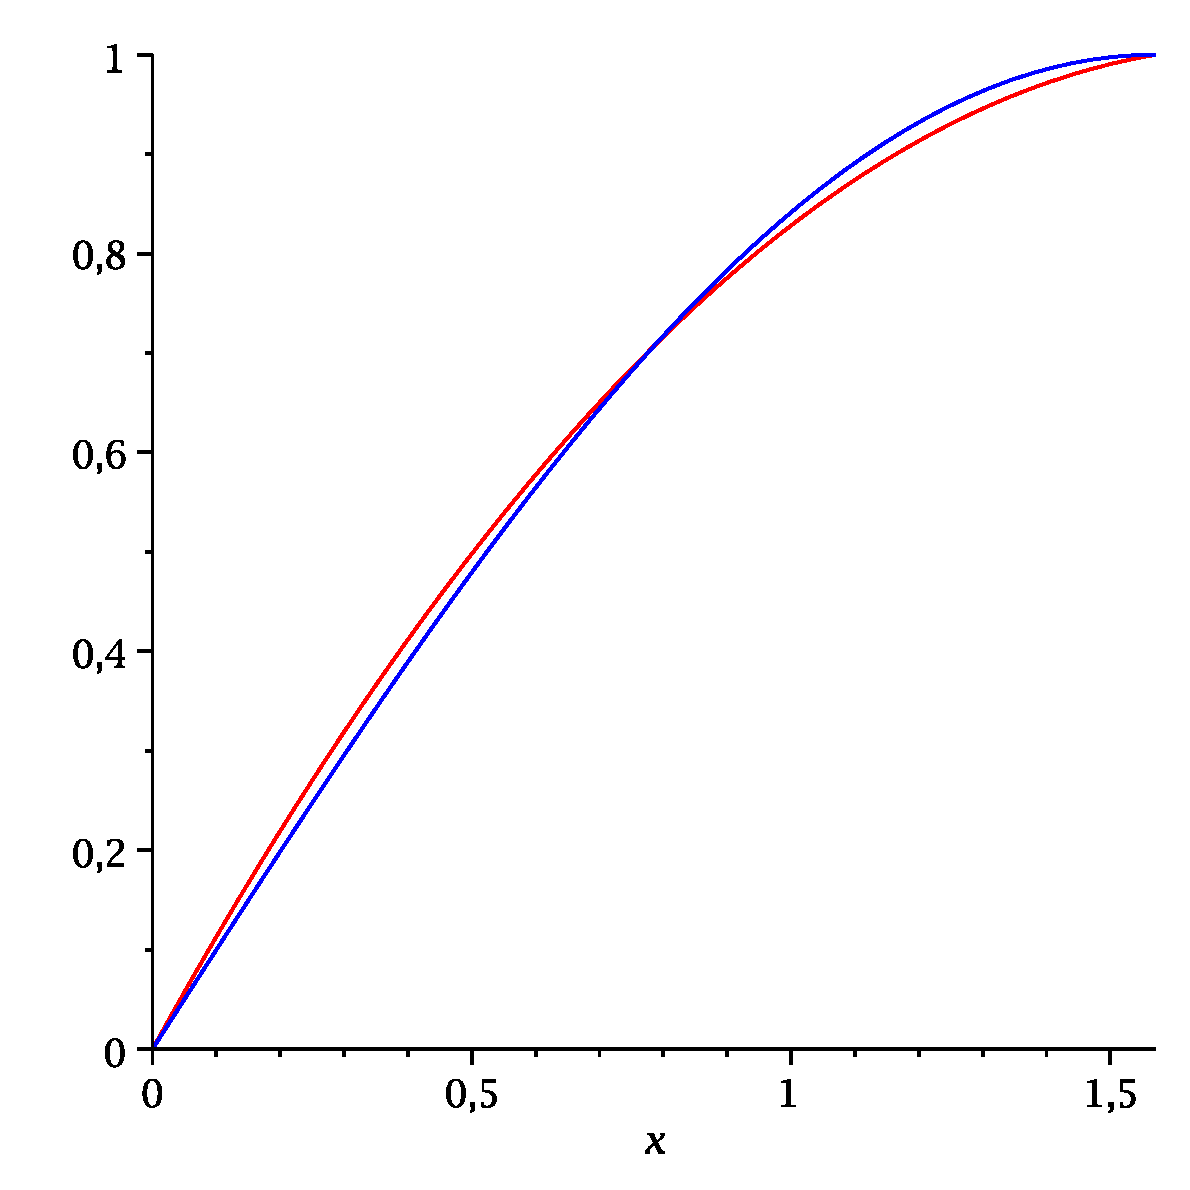
\includegraphics[scale=0.23]{seno.eps} & 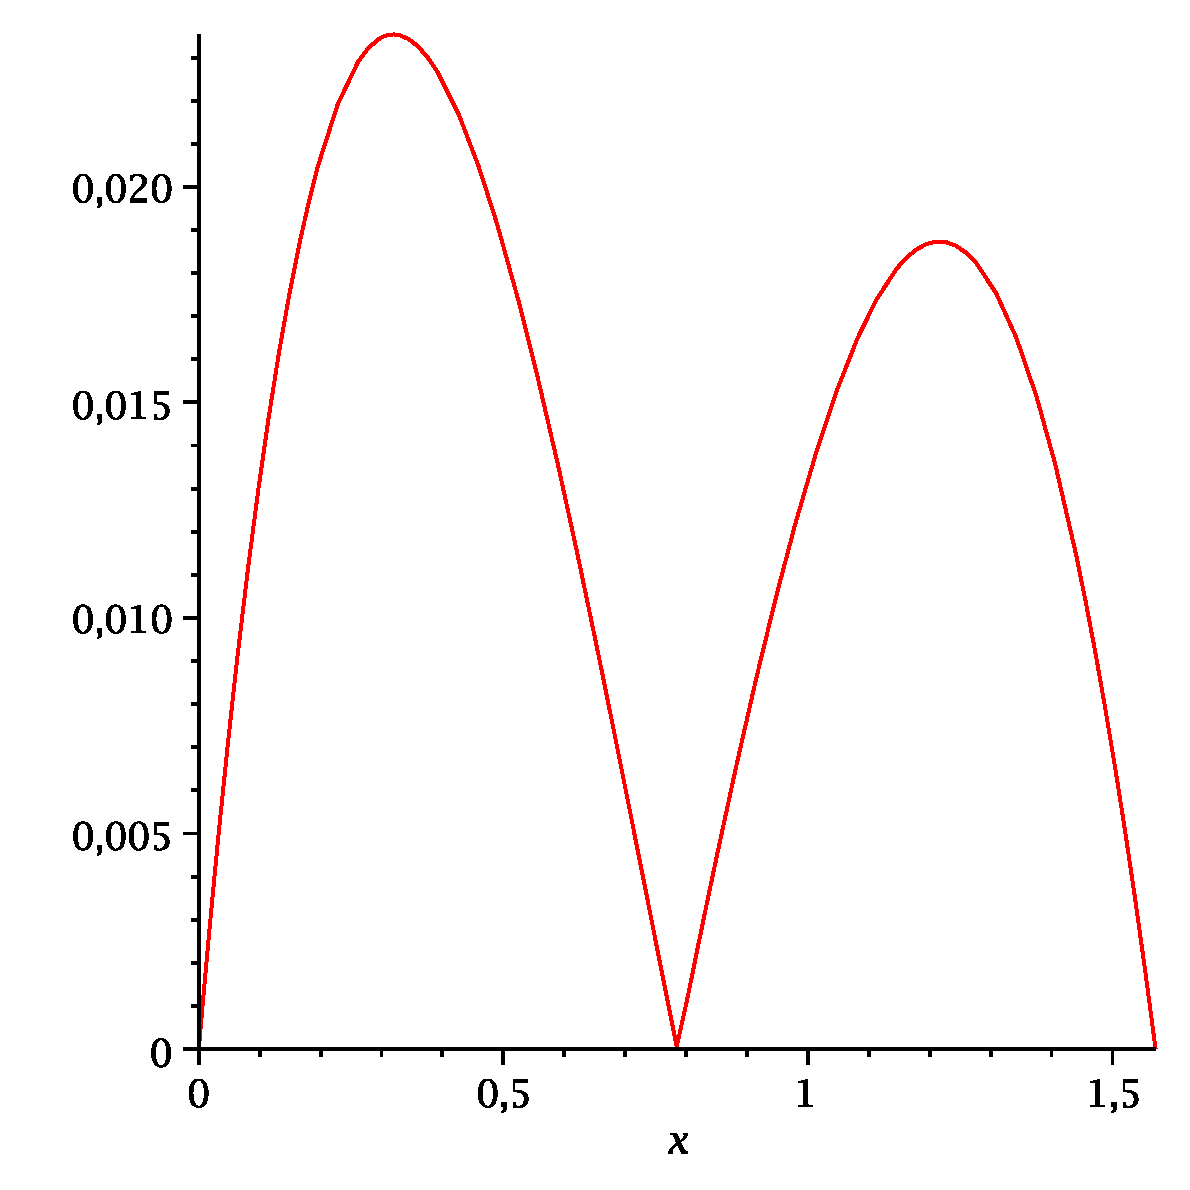
\includegraphics[scale=0.23]{errorseno.eps}\\
\textcolor{red}{\sin(x)} \text{ vs }\textcolor{blue}{P_2(x)} & |E(x)|=|f(x)-P_2(x)|
\end{array}
$$
}
% %%%%
\frame
{
\frametitle{Ejemplo:}
Obtener el polinomio interpolador para la funci\'on $f(x) = \sin(x)$ sobre el soporte formado por los puntos:
$$
x=\left\{0,\frac{\pi}{6},\frac{\pi}{4},\frac{\pi}{3},\frac{\pi}{2}\right\}
$$
\uncover<2->{
Tabla del ejercicio anterior
\begin{block}{}
$$
\begin{array}{ccccc}
 0 &  \rightarrow & 0 & &\\
 \frac{\pi}{4} & \rightarrow & 0.707 & 0.90 &\\
 \frac{\pi}{2} & \rightarrow & 1 & 0.373 & -0.336\\
\end{array}
$$
\end{block}
}
\uncover<3->{
Se agregan los nuevos nodos al final de la tabla y queda:
\begin{block}{}
$$
\begin{array}{ccccccc}
 0 &  \rightarrow & 0 & & &\\
 \frac{\pi}{4} & \rightarrow & 0.707 & 0.90 & &\\
 \frac{\pi}{2} & \rightarrow & 1 & 0.373 & -0.336 & &\\
 \frac{\pi}{6} & \rightarrow & 0.5 & 0.477 & -0.399 & -0.121 &\\
 \frac{\pi}{3} & \rightarrow & 0.867 & 0.699 & -0.423 & -0.091 & 0.0288
\end{array}
$$}
\end{block}
}
% %%%
\frame
{
\frametitle{Ejemplo:}
Formando el polinomio interpolante de Newton
\scriptsize
$$
P_4(x) = P_2(x) - 0.121(x-0)(x-\pi/4)(x-\pi/2)+ 0.0228(x-0)(x-\pi/4)(x-\pi/2)(x-\pi/6)
$$
\uncover<2->{
$$
\begin{array}{cc}
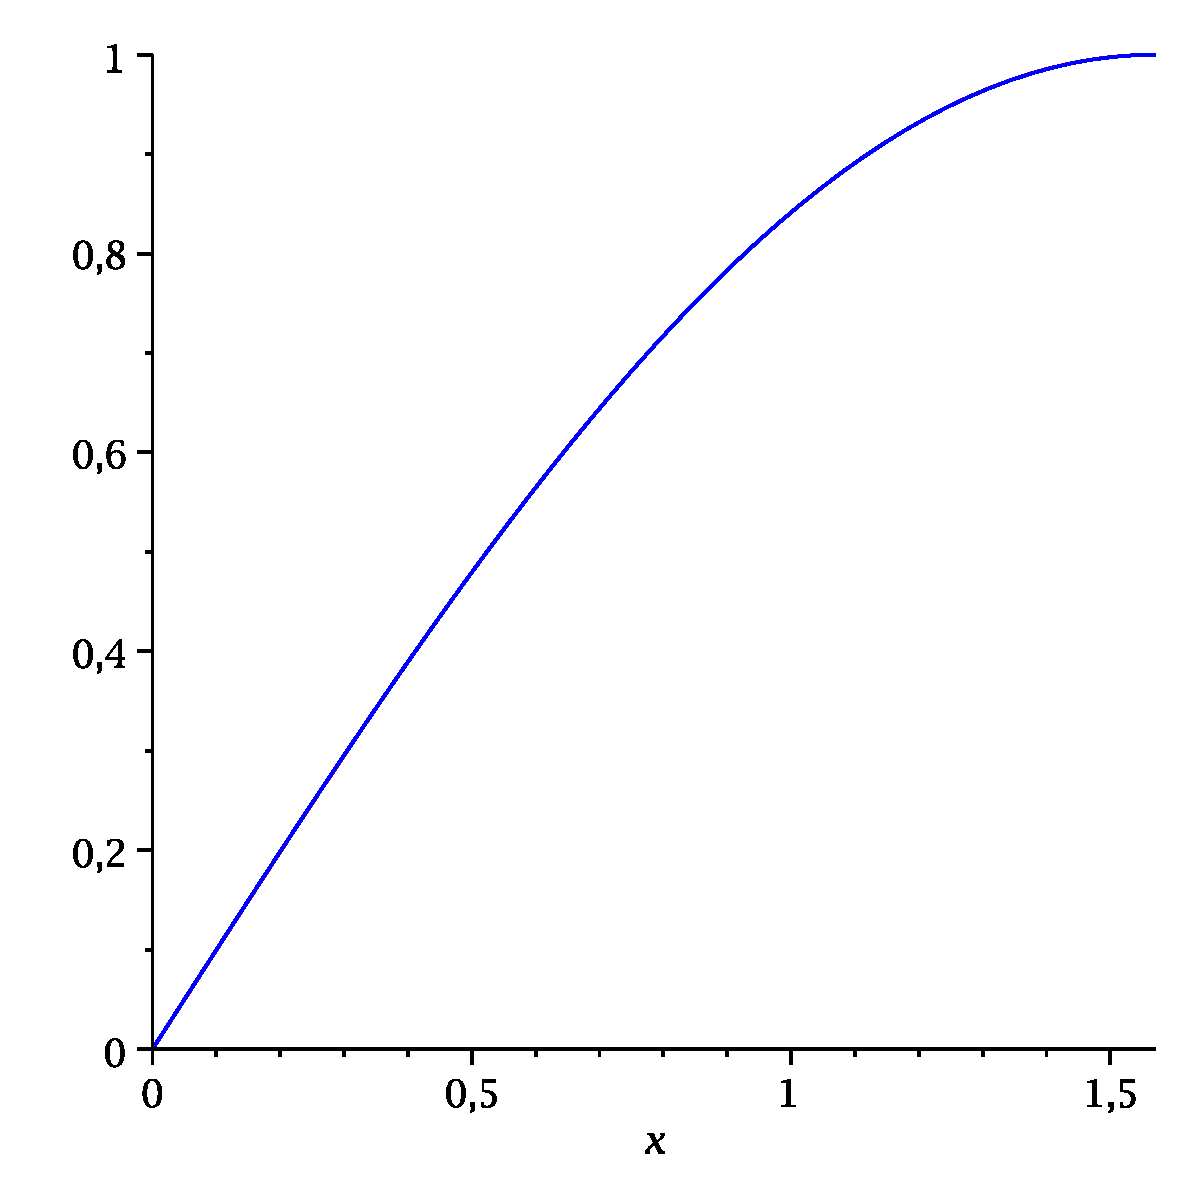
\includegraphics[scale=0.23]{seno4.eps} & 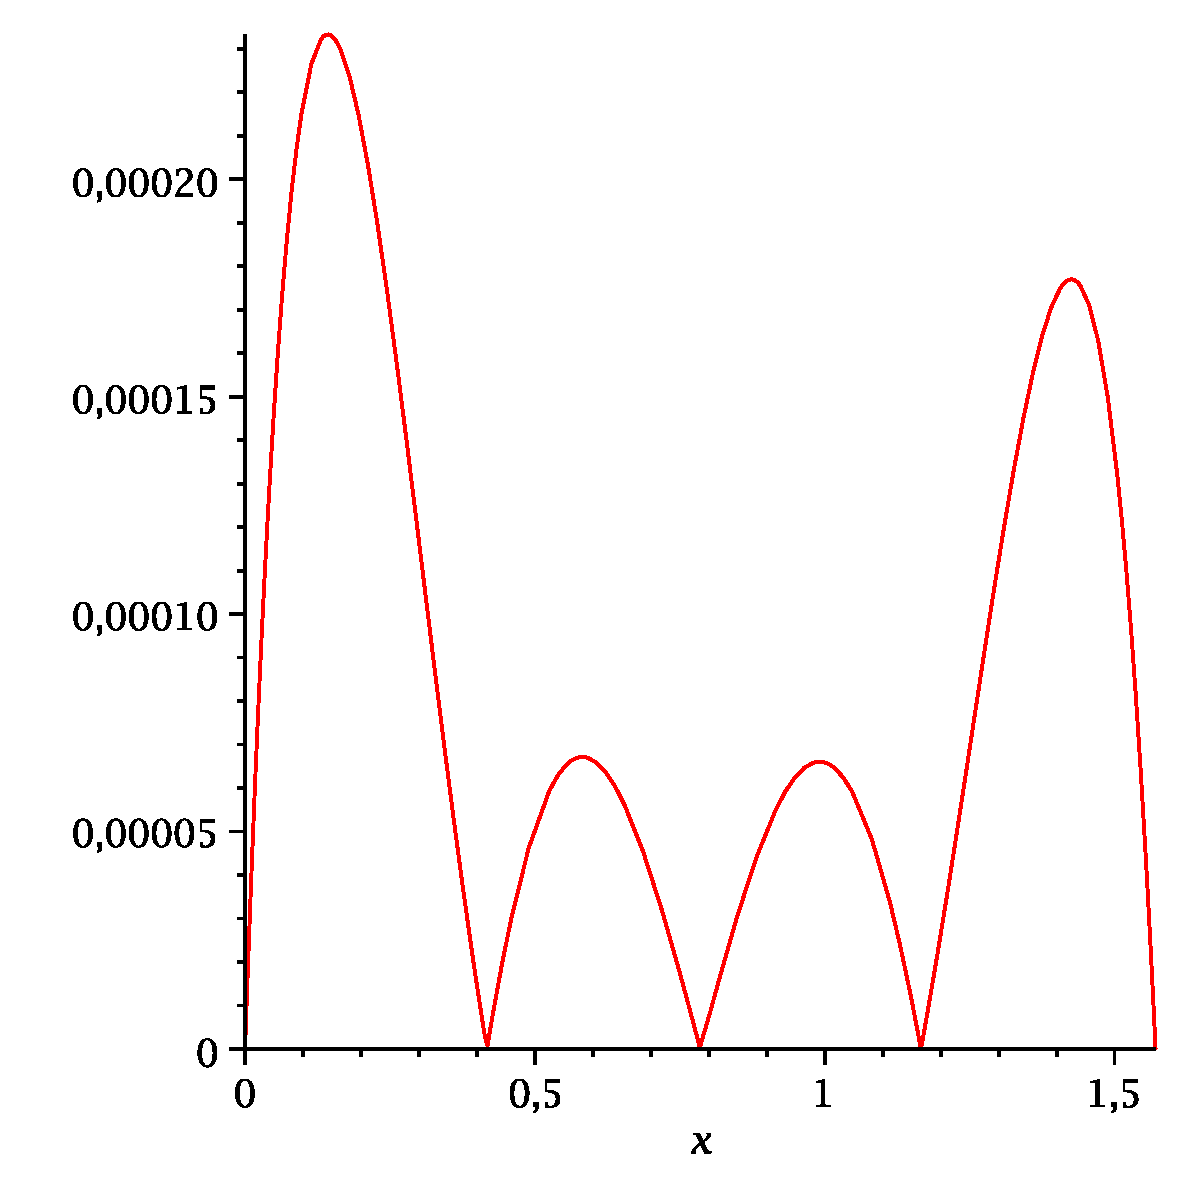
\includegraphics[scale=0.23]{errorseno4.eps}\\
\textcolor{red}{\sin(x)} \text{ vs }\textcolor{blue}{P_4(x)} & |E(x)|=|f(x)-P_4(x)|
\end{array}
$$
}
}
% %%%%
\frame{
\frametitle{Cota de error para el polinomio de Newton}
\begin{block}{Teorema:}
Sea $f \in \mathcal{C}^{n+1}[a, b]$ y $p$ el polinomio de grado $\leq n$ que interpola a $f$ en los $n + 1$ puntos $x_0, x_1, \ldots , x_n$ del intervalo $[a, b]$. Entonces
$$
f(x)-p(x) = \mathcal{F}[x_0,x_1,\ldots,x_n,x]\prod_{i=0}^n(x-x_i)
$$\end{block}
\uncover<2->{
\textbf{Demostraci\'on:}
Por el Teorema del Residuo, existe $\xi = \xi(x)$ tal que
$$
f(x)-p(x) = \dfrac{1}{(n+1)!}f^{(n+1)}(\xi)\prod_{i=0}^n(x-x_i)
$$}
\uncover<3->{
Por otra parte, el polinomio de interpolaci\'on de Newton est\'a dado por
$$
p(x) = \mathcal{F}[x_0] + \mathcal{F}[x_0,x_1](x - x_0 ) +  \cdots + \mathcal{F}[x_0,x_1,\ldots,x_n](x - x_0 )\cdots(x - x_{n-1})
$$
}
}
% %%%%%
\frame{
\frametitle{Cota de error para el polinomio de Newton}
El polinomio de Newton que interpola a $f$ en $x_0, x_1, \ldots , x_n, x$:
$$
p(x) = \mathcal{F}[x_0] + \mathcal{F}[x_0,x_1](x - x_0 ) +  \cdots + \mathcal{F}[x_0,x_1,\ldots,x_n,x](x - x_0 )\cdots(x - x_n)
$$
\uncover<2->{
y por tanto
\begin{block}{}
$$
f(x)-p(x) = \mathcal{F}[x_0,x_1,\ldots,x_n,x]\prod_{i=0}^n(x-x_i)
$$
\end{block}}
\uncover<3->{
De esta manera se puede concluir que:
$$
\mathcal{F}[x_0,x_1,\ldots,x_n,x] = \dfrac{1}{(n+1)!}f^{(n+1)}(\xi(x))
$$
}
}
% %%%%
\frame{
\frametitle{Observaciones}
\begin{itemize}
\item<1-> Si $p_n$ interpola a $f$ en los $n + 1$ puntos $x_0, x_1, \ldots , x_n$,
$$
f(x)-p(x) =\dfrac{1}{(n+1)!}f^{(n+1)}(\xi)\prod_{i=0}^n(x-x_i)
$$
con $\xi \in [x_0, x_n]$.
\item<2-> $\xi$ es desconocido y la f\'ormula del error s\'olo es \'util si la derivada est\'a acotada.
\item<3-> Si $|f^{(n+1)}(x)|<M$ y $h=\max\{x_{i+1}-x_i:i=0,\ldots,n\}$
$$
\max_{x \in [x_0,x_n]}|f(x)-p(x)| \leq \dfrac{Mh^{n+1}}{(n+1)!}
$$
\item<4-> El error disminuye a medida que $n$ crece y $h$ disminuye, s\'olo si $|f^{(n+1)}(x)|$ est\'a acotada.
\item<5-> Aumentar el grado del polinomio no garantiza una mejor aproximaci\'on (pueden aparecer oscilaciones entre los puntos de interpolaci\'on)
\end{itemize}
}
% %%%%
\frame{
\frametitle{Observaciones}
\begin{itemize}
\item<1-> Por fuera del intervalo que contiene a los puntos de interpolaci\'on,
$$
\prod_{i=0}^n(x-x_i)
$$
puede crecer ``r\'apido'' (extrapolaci\'on)
\item<2-> En el interior del intervalo aumentar los puntos de interpolaci\'on no implica mejorar la aproximaci\'on.
\item<3-> Al aumentar el grado del polinomio, aumentan las oscilaciones.
\item<4-> Hasta ahora las aproximaciones de los polinomios de interpolaci\'on no dependen de la distribuci\'on de los puntos $x_0,\ldots,x_n$ de interpolaci\'on.
\item<5-> Puntos de interpolaci\'on igualmente espaciados a menudo conducen a resultados err\'oneos en los extremos.
\end{itemize}
}
% %%%%
\frame{
\frametitle{Interpolaci\'on de Newton con puntos igualmente espaciados}
\begin{itemize}
\item<1-> Sea $f$ una funci\'on definida en algunos puntos $x_0,\ldots, x_n$. Denotando por $y_0, \ldots, y_n$ sus valores correspon-
dientes. Recordamos la f\'ormula de Newton para el polinomio interpolante que tiene valores
$y_i = f(xi)$ en los puntos $x_i$:
$$
P(x) = \sum_{k=0}^n \mathcal{F}[x_0,\ldots,x_k]\prod_{j=0}^{k-1}(x - x_k )
$$
\item<2-> Las diferencias divididas $\mathcal{F}[x_0,\ldots,x_k]$ se definen de manera recursiva:
\small{
$$
\mathcal{F}[x_i]=f(x_i)=y_i,\qquad\mathcal{F}[x_i,\ldots,x_j] = \dfrac{\mathcal{F}[x_{i+1},\ldots,x_j]-\mathcal{F}[x_i,\ldots,x_{j-1}]}{x_j-x_i}
$$}
\end{itemize}
}
% %%%%%
\frame{
\frametitle{Interpolaci\'on de Newton con puntos igualmente espaciados}
\begin{itemize}
\item<1-> Considerando el caso particular
cuando los puntos $x_0,\ldots,x_n$ son equidistantes:
$$
x_k = x_0 + kh,\qquad k=0,1,\ldots,n
$$
\item<2-> Planteando el cambio de variables
$$
x=x_0+th \quad\text{con }t\in(0,n)
$$
\item<3-> Obtenemos entonces que
$$
x-x_1 = (t-1)h; \quad x-x_2=(t-2)h; \quad \ldots \quad; x-x_{n-1} = (t-n+1)h 
$$
\end{itemize}
}
% %%%%
\frame{
\frametitle{Interpolaci\'on de Newton con puntos igualmente espaciados}
\begin{block}{Definici\'on: Diferencia Finita Progresiva}
  Se define como diferencia finita progresiva de una funci\'on $f(x)$ en un punto $x_0$, y
  se
  representa $\Delta f (x_0)$ a la diferencia:
  $$
  \Delta f(x_0) = f(x_1) - f(x_0)
  $$
\end{block}
\uncover<2->{
  Del mismo modo se puede definir la de
segundo orden:
$$
\Delta^2f(x_0) = \Delta f(x_1) - \Delta f(x_0) = f(x_2) -2f(x_1) + f(x_0)
$$

En general:
$$
\Delta^k f(x_0) = \Delta^{k-1}f(x_1) - \Delta^{k-1}f(x_0)
$$
}}
% %%%%
\frame{
\frametitle{Interpolaci\'on de Newton con puntos igualmente espaciados}
\begin{itemize}
\item<1-> La relaci\'on entre las diferencias finitas progresivas y las diferencias divididas viene dada por:
{\small
\begin{eqnarray}
 \nonumber f[x_0,x_1] & = & \dfrac{f(x_1) - f(x_0)}{x_1 - x_0} = \dfrac{\Delta f(x_0)}{h} \Rightarrow \Delta f(x_0) =
hf[x_0,x_1]\\
\nonumber f[x_0,x_1,x_2] & = & \dfrac{f[x_1,x_2] - f[x_0,x_1]}{x_2 - x_0} = \dfrac{\Delta f(x_1) - \Delta f(x_0)}{2h^2}\\
\nonumber&\Rightarrow& \Delta^2 f(x_0) = 2h^2f[x_0,x_1,x_2]
\end{eqnarray}}
En general
$$
\Delta^nf(x_0) = n!h^nf[x_0,x_1,\ldots,x_n]
$$
\end{itemize}
}
% %%%%
\frame{
\frametitle{Interpolaci\'on de Newton con puntos igualmente espaciados}
\begin{itemize}
\item<1-> A partir de la f\'ormula de Newton con diferencias divididas y de la relaci\'on entre estas \'ultimas y las diferencias finitas
progresivas se tiene:
\end{itemize}
\footnotesize{
$$
 P_n(x) = f[x_0] + f[x_0,x_1] (x - x_0 ) 
 $$
 $$
 + f[x_0,x_1,x_2](x - x_0 )(x - x_1 ) + \cdots + f[x_0,x_1,\ldots,x_n](x - x_0 )(x -
x_1 ) \cdots (x - x_{n-1} )
$$}
\normalsize
\begin{itemize}
\item<2-> A partir del cambio de variable $x = x_0 + th$ se tiene que
\end{itemize}
\footnotesize{
\uncover<2->{$$
P_n(x_0+th) = Q_n(t)
$$
$$
=f(x_0)+\dfrac{\Delta f(x_0)}{h}th +\dfrac{\Delta^2
f(x_0)}{2!h^2}t(t-1)h^2+\cdots+\dfrac{\Delta^nf(x_0)}{n!h^n}t(t-1)\cdots(t-n+1)h^n
$$
$$
= f(x_0)+\Delta f(x_0)t +\dfrac{\Delta^2f(x_0)}{2!}t(t-1)+\cdots+\dfrac{\Delta^nf(x_0)}{n!}t(t-1)\cdots(t-n+1)
$$
$$
= \sum_{k=0}^n\dfrac{\Delta^kf(x_0)}{k!}t(t-1)\cdots(t-k+1)=\sum_{k=0}^n\Delta^kf(x_0)\binom{t}{k}
$$
}}}
% %%%%
\frame{
\frametitle{Ejemplo:}
\begin{itemize}
\item<1-> Construir el polinomio $P$ de grado $\leq 3$ que en los puntos $-1/2; 0; 1/2; 1$
tome los valores $-4; 3; 13/2; 8$.
\item<2-> Construyendo la tabla de diferencias divididas se obtiene:
$$
\begin{array}{|c|c|c|c|c|}
\hline
x & \Delta^0 f(x) = f(x) & \Delta f(x) & \Delta^2 f(x) & \Delta^3 f(x)\\\hline
-1/2 & \color{red}-4 & &  &\\ \hline
0 & 3 & \color{red}7 &  &  \\ \hline
1/2 & 13/2 & 7/2 & \color{red}-7/2 &  \\ \hline
1 & 8 & 3/2 & -2 & \color{red}3/2  \\ \hline
\end{array}
$$
\item<3-> El polinomio $Q_n(t)$ viene dado por:
\footnotesize{
\begin{eqnarray}
\nonumber Q_n(t) = P\left(\frac{-1}{2} + \frac{t}{2}\right) & = & \sum_{k=0}^n\Delta^kf(x_0)\binom{t}{k}\\
\nonumber& = & -4 + 7t - \dfrac{7}{2}\dfrac{t(t-1)}{2} + \dfrac{3}{2}\dfrac{t(t-1)(t-2)}{6}\\
\nonumber& = & -4 + \dfrac{37t}{4} - \frac{5t^2}{2}+\dfrac{t^3}{4}
\end{eqnarray}
}
\end{itemize}
}
% %%%%%
\frame{
\frametitle{Ejemplo:}
\begin{itemize}
\item<1-> El polinomio $P(x)$ viene dado por:
$$
P(x) = Q(2x+1) = 3+10x-7x^2+2x^3
$$
\end{itemize}
}
% %%%%
\frame{
\frametitle{Fen\'omeno de Runge}
Polinomios interpolantes para la funci\'on de Runge
$$
f(x) = \dfrac{1}{1+25x^2}, \qquad x \in [-1,1]
$$
sobre puntos igualmente espaciados no converge
\begin{center}
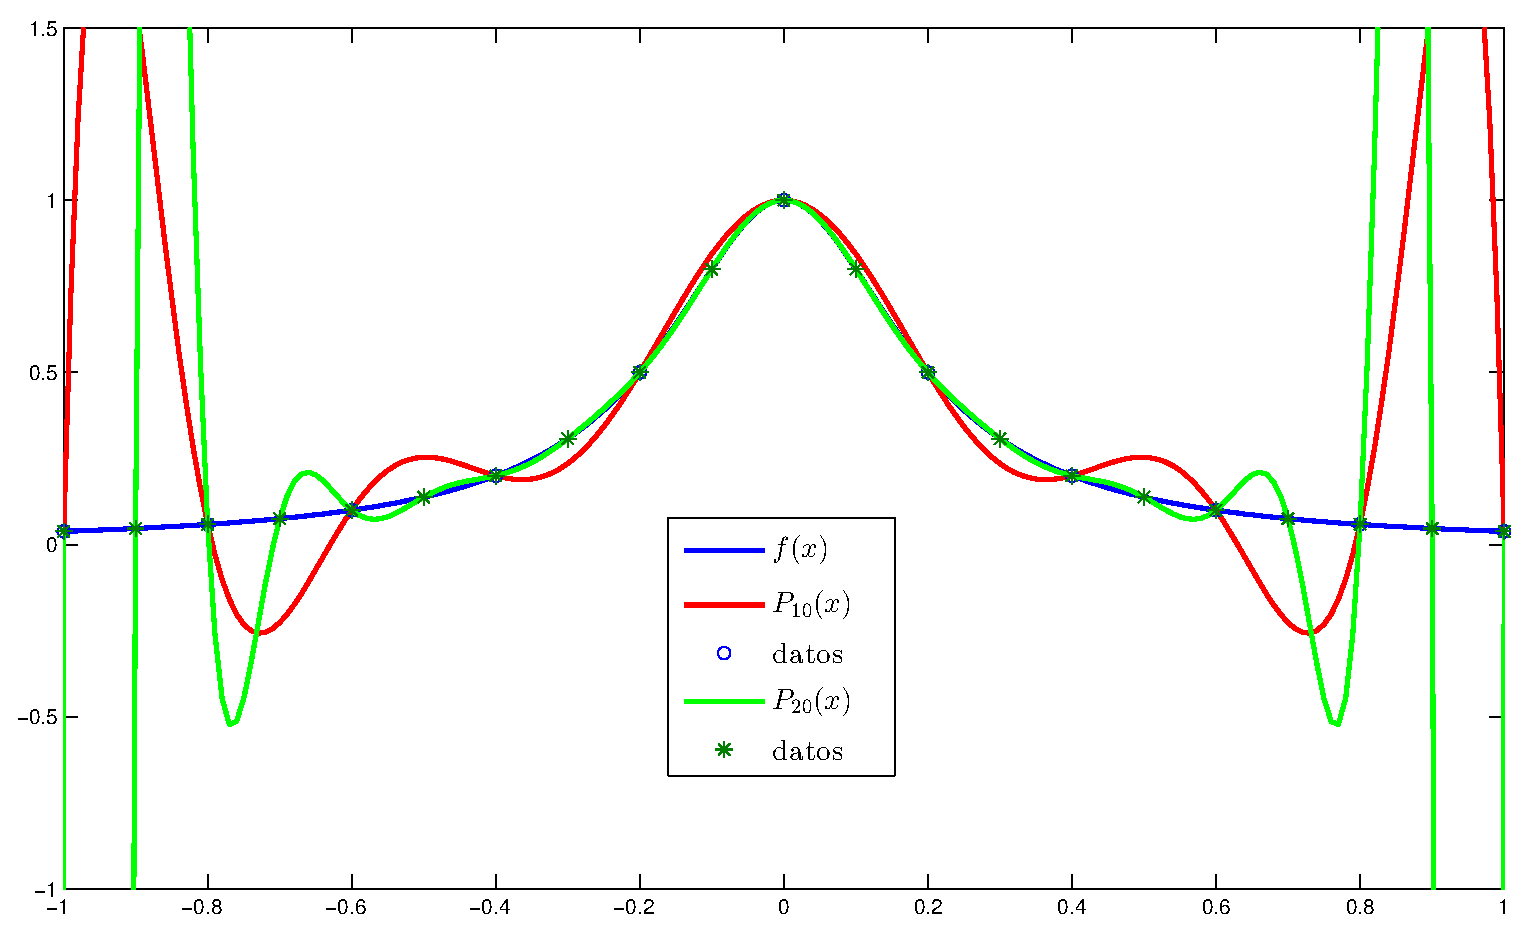
\includegraphics[scale=0.35]{rungeinter.eps}
\end{center}
}
%%%%
\frame{
\frametitle{Fen\'omeno de Runge}
Los puntos de interpolaci\'on se pueden distribuir no uniformemente con el fin de minimizar el fen\'omeno de Runge
$$
x_i = \cos\left(\dfrac{2i+1}{2n+2}\pi\right), \qquad i=0,\ldots,n-1
$$
\begin{center}
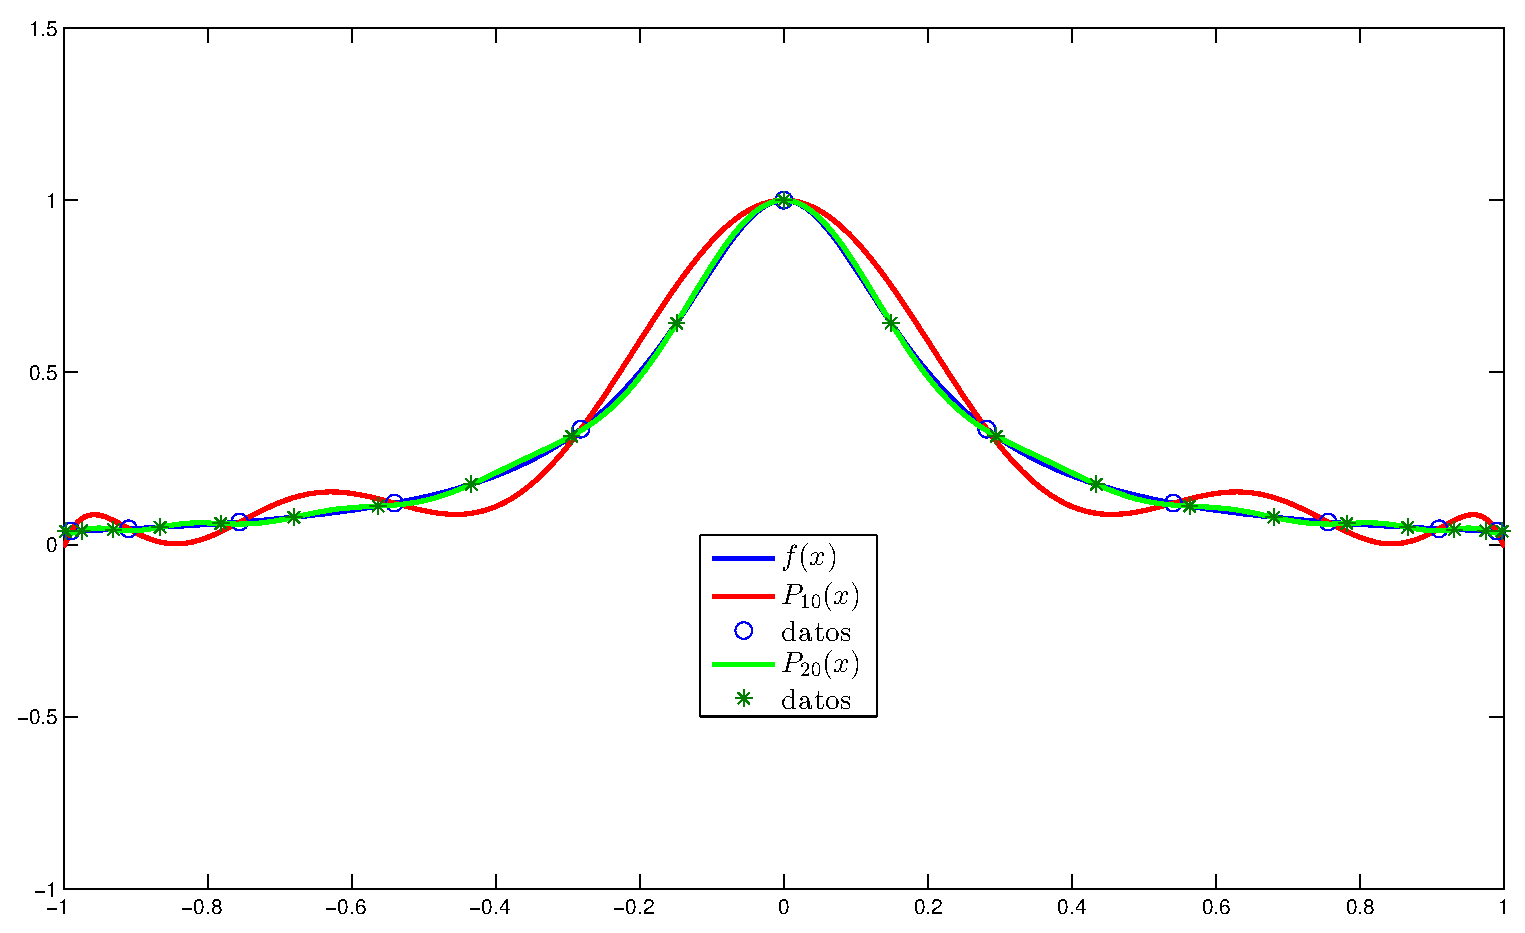
\includegraphics[scale=0.35]{rungecheby.eps}
\end{center}
}
%%%%
\subsection{Interpolaci\'on de Chebyshev}
\frame{
\frametitle{Interpolaci\'on de Chebyshev}
\begin{block}{}
Dada una funci\'on $f(x)$ definida en un intervalo $[a, b]$, la mejor aproximaci\'on polin\'omica de grado $n$ ser\'a aquella que minimice
$$
E[q(x)] \equiv \max_{x \in [a,b]}|f(x)-q(x)|
$$
\end{block}
Si un determinado polinomio $Q_n(x)$ hace que $E[Qn(x)]$ sea el de valor m\'inimo entre todos los polinomios de grado $n$ entonces se dice
$Q_n(x)$ es la aproximaci\'on minimax de grado $n$ de la funci\'on $f(x)$ en $[a, b]$.
}
%%%%
\frame
{\frametitle{Interpolaci\'on de Chebyshev}
\begin{block}{Polinomios de Chebyshev: definici\'on}
El polinomio de Chebyshev de orden $n$-\'esimo se define como
$$
T_n(x) = \cos(n\arccos(x)), x\in [-1,1], n=0,1,2\ldots
$$
\end{block}
\uncover<2->{
La definici\'on anterior establece una relaci\'on de recurrencia:
$$
T_0(x) = \cos(0) = 1 \mbox{ y } T_1(x)=\cos(\arccos(x))=x
$$
$$
T_n(x) = \cos(n\underbrace{\arccos(x)}_{\theta})=\cos(n\theta), \quad \theta \in [0,\pi]
$$
de lo cual}
\uncover<3->{
\begin{eqnarray}
T_{n+1}(x) & = & \cos((n+1)\theta) = \cos(n\theta)cos(\theta) - \sin(n\theta)\sin(\theta)\nonumber\\
T_{n-1}(x) & = & \cos((n-1)\theta) = \cos(n\theta)cos(\theta) + \sin(n\theta)\sin(\theta)\nonumber
\end{eqnarray}
y al sumar las dos \'ultimas con $x = \cos(\theta)$,}
\uncover<4->{
\begin{eqnarray}
T_{n+1}(x) + T_{n-1}(x) & = & 2cos(n\theta)\cos(\theta)\nonumber\\
T_{n+1}(x) & = & 2\cos(\theta)\cos(n\theta) - T_{n-1}(x)\nonumber\\
T_{n+1}(x) & = & 2xT_n(x) - T_{n-1}(x)\nonumber
\end{eqnarray}}
}
%%%%
\frame
{
\frametitle{Polinomios de Chebyshev: propiedades}
\begin{enumerate}
  \item<1-> Relaci\'on de recurrencia de tres t\'errminos para los polinomios de Chebyshev:
$$
T_{n+1}(x) = 2xT_n(x)-T_{n-1}(x), n=0,1,2\ldots
$$
siendo los valores iniciales de la recurrencia
$$
\begin{array}{lcl}
T_0(x) &=& 1\\
T_1(x) &=& x\\
\uncover<2->{T_2(x) &=& 2xT_1(x) - T_0(x) = 2x^2 - 1}\\
\uncover<3->{T_3(x) &=& 2xT_2(x) - T_1(x) = 4x^3 - 3x}\\
\uncover<4->{T_4(x) &=& 2xT_3(x) - T_2(x) = 8x^4 - 8x^2 + 1}\\
\end{array}
$$
\item<5-> El coeficiente del t\'ermino $x^n$ en $T_n(x)$ es $2^{n-1}$ y se cumple que $T_n(-x) = (-1)^nT_n(x)$.
\item<6-> Los $n$ ceros de $T_n(x)$ est\'an en el intervalo $[-1, 1]$ y est\'an dados por
$$
x_k = \cos \left( \frac{2k+1}{2n+2}\pi \right), k= 0,1,\ldots,n-1
$$
$T_n(x)$ tiene $n + 1$ extremos en el intervalo $[-1, 1]$ que vienen dados por $x'_k = \cos(\frac{k\pi}{n})$, $k= 0,\ldots, n$, donde los
polinomios valen: $T(x'_k) = (-1)^k$
\end{enumerate}
}
%%%%%
\frame{
  \frametitle{Ejemplo:}
}
%%%%%
\subsection{Interpolaci\'on a trozos}
\frame{
  \frametitle{Interpolaci\'on a trozos}
\begin{itemize}
\item $S(x)$ En un polinomio interpolador de grado $n$ es posible tener $n-1$ extremos relativos, lo cual trae como consecuencia que tenga
muchas oscilaciones o fluctuaciones al pasar por los puntos dados.
\item<2-> Una alternativa para evitar dichas fluctuaciones es generar polinomios $S_k(x)$ que solo interpolen dos nodos consecutivos y luego unirlos en sus extremos.
\item<3-> El conjunto $\{S_k(x)\}$ forman
una curva polinomial a trozos o spline que se denota $S(x)$.
\end{itemize}
\uncover<4->{
\begin{figure}[ht]
  \begin{center}
    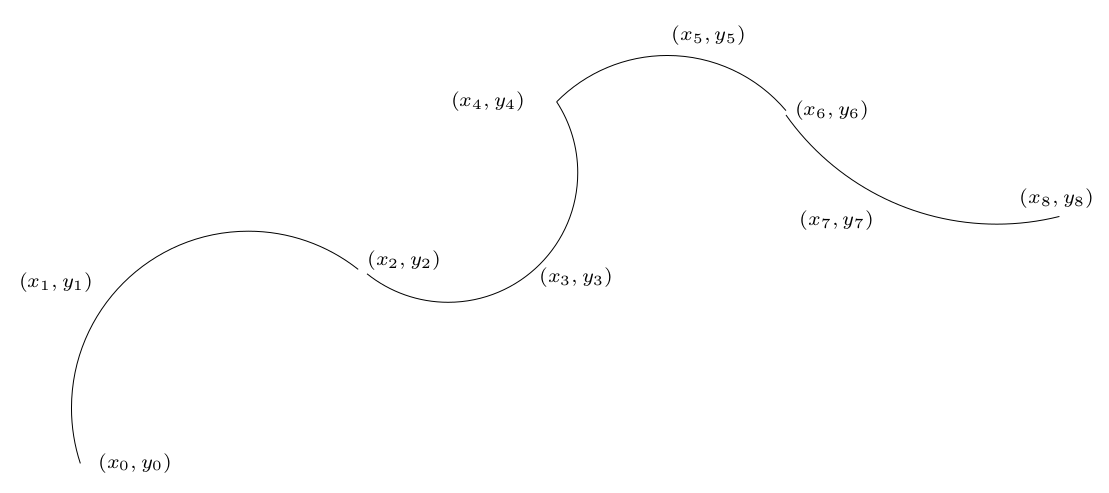
\includegraphics[scale=0.25]{splines.png}
  \caption{Interpolaci\'on a Trozos.}
  \end{center}
\end{figure}
}}
%%%%%
\frame{
  \frametitle{Interpolaci\'on Lineal a trozos}
\begin{itemize}
\item<1-> Sean $(x_0,y_0), (x_1,y_1), (x_2,y_2),\ldots,(x_k,y_k),(x_{k+1},y_{k+1}),\ldots,(x_n,y_n)$, los puntos por los cuales debe pasar el polinomio interpolador
\item<2-> El polinomio m\'as simple que se puede construir es el polinomio de grado uno, el cual produce una l\'inea poligonal.

\begin{figure}[ht]
\begin{center}
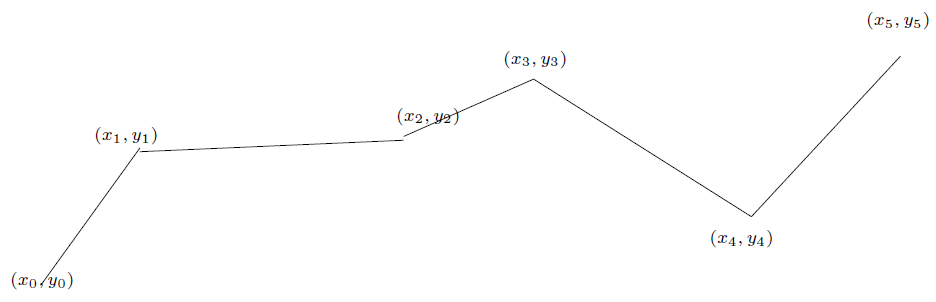
\includegraphics[scale=0.45]{inter_lin_troz.png}
\end{center}
\caption{Interpolaci\'on Lineal a Trozos.}
\end{figure}
\end{itemize}
}
%%%%%
\frame{
\frametitle{Interpolaci\'on Lineal a trozos}
\begin{itemize}
\item Por los polinomios interpoladores de Lagrange se puede determinar cada uno de los segmentos que forman est\'a l\'inea poligonal.
\item<2-> Si $S_k(x)$ es el k-\'esimo segmento que une los puntos $(x_k,y_k),(x_{k+1},y_{k+1})$ se tiene entonces que
$$
S_k(x) = y_k\dfrac{x-x_{k+1}}{x_k-x_{k+1}}+y_{k+1}\dfrac{x-x_k}{x_{k+1}-x_k}
$$
o tambi\'en
$$
S_k(x) = y_k + d_k(x-x_k), \qquad d_k=\dfrac{y_{k+1}-y_k}{x_{k+1}-x_k}
$$
\end{itemize}
}
%%%%%
\frame{
\frametitle{Interpolaci\'on Lineal a trozos}
\begin{itemize}
\item<1-> Que es la ecuaci\'on de la recta que pasa por los puntos dados, luego entonces,
$$
S(x) = \left\{\begin{array}{ll}
               S_0(x) = y_0 + d_0(x-x_0), & x \in [x_0,x_1]\\
               S_1(x) = y_1 + d_1(x-x_1), & x \in [x_1,x_2]\\
               \vdots & \vdots\\
               S_k(x) = y_k + d_k(x-x_k), & x \in [x_k,x_{k+1}]\\
               \vdots & \vdots\\
               S_{n-1}(x) = y_{n-1} + d_{n-1}(x-x_{n-1}), & x \in [x_{n-1},x_n]\\
              \end{array}
\right.
$$
\end{itemize}
}
%%%%
\frame{
\frametitle{Interpolaci\'on Lineal Segmentaria}
\begin{block}{Evaluaci\'on}
 \begin{itemize}
  \item Localizar el intervalo tal que $x \in [x_i, x_{i+1}]$. (Algoritmo de localizaci\'on).
  \item<2-> $S_i(x) = y_i+(x-x_i)\dfrac{y_{i+1}-y_i}{x_{i+1}-x_i}$, $x_i\leq x\leq x_{i+1}$, $i=0,\ldots,n-1$
 \end{itemize}
\end{block}

\uncover<3->{
\begin{block}{Error}
 Si $y_i = f(x_i)$ con $f \in \mathcal{C}^2[a,b]$:
 $$
 |S(x)-f(x)| \leq \dfrac{1}{8}h^2\max_{x \in [x_0,x_n]}|f''(x)| = O(h^2)
 $$
donde $h$ es la distancia m\'axima entre dos nodos adyacentes.
\end{block}}

\uncover<4->{
\begin{block}{Derivada}
 \begin{eqnarray}
  S'(x) = \dfrac{y_{i+1}-y_i}{x_{i+1}-x_i} && x_i<x<x_{i+1}, i=0,1,\ldots,n-1\nonumber\\
  |S'(x)-f'(x)| = O(h) && x\neq x_i,x_0<x<x_n\nonumber
 \end{eqnarray}
\end{block}
}}
%%%%
\frame{
\frametitle{Funci\'on de Runge $f(x) = \dfrac{1}{1+x^2}$}
\begin{block}{$S(x)$ interpolante lineal segmentaria determinado en $n + 1$ nodos equidistantes}
\begin{minipage}{5cm}
 \begin{center}
  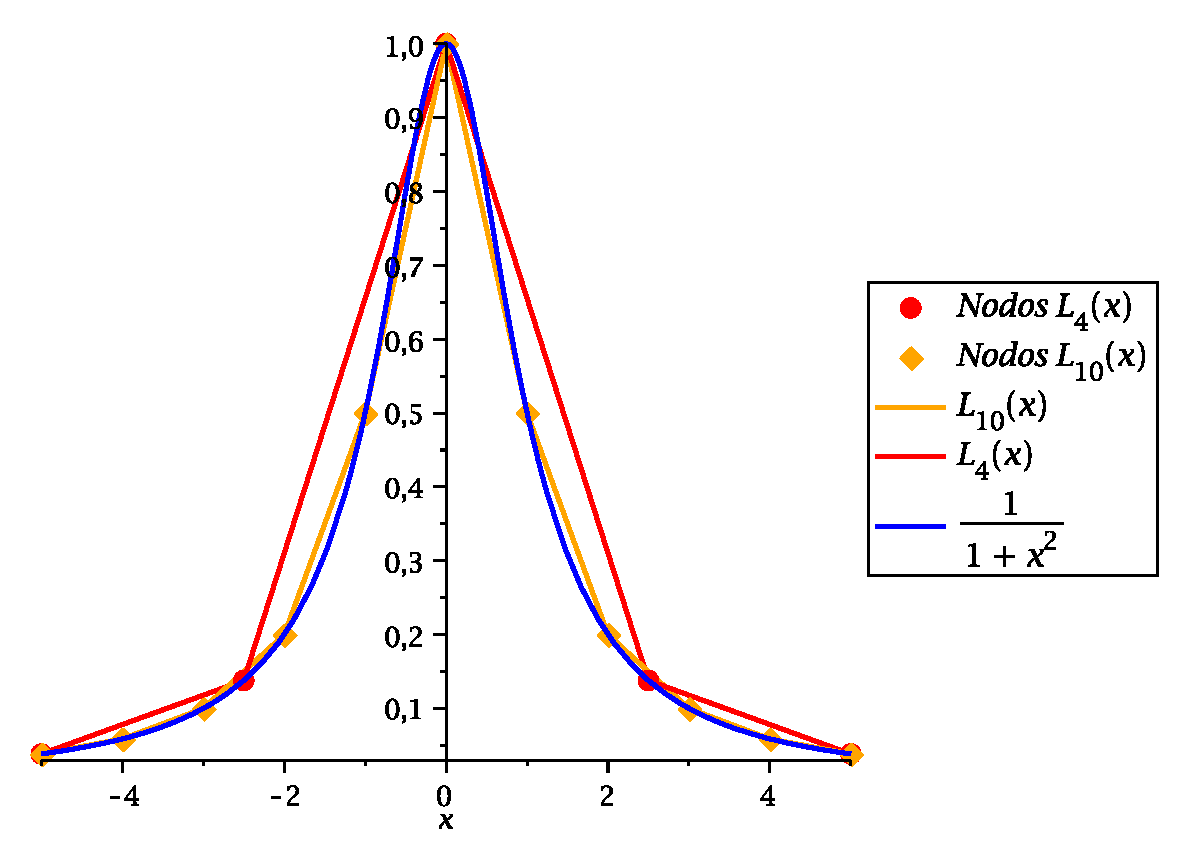
\includegraphics[scale=0.3]{linear_seg.eps}
 \end{center}
\end{minipage}
\begin{minipage}{6.5cm}
$$
x_j = -5+j\dfrac{10}{n}, j=0,1,\ldots,n
$$
\begin{center}
\begin{tabular}{|c|c|}\hline
 $n$ & $\|f-S\|_{\infty}$\\\hline
 50 & 9.33e-03\\\hline
100 & 2.46e-03\\\hline
200 &  6.22e-04\\\hline
400 &  1.50e-04\\\
800 &  3.75e-05\\\hline
1600 &  9.37e-06\\\hline
3200 & 2.34e-06\\\hline
6400 &  5.86e-07\\\hline
\end{tabular}
 \end{center}
\end{minipage}
\end{block}
}
%%%%
\frame{
\frametitle{Funci\'on de Runge $f(x) = \dfrac{1}{1+x^2}$}
\begin{block}{Error del interpolante lineal segmentaria 5 nodos.}
 \begin{center}
  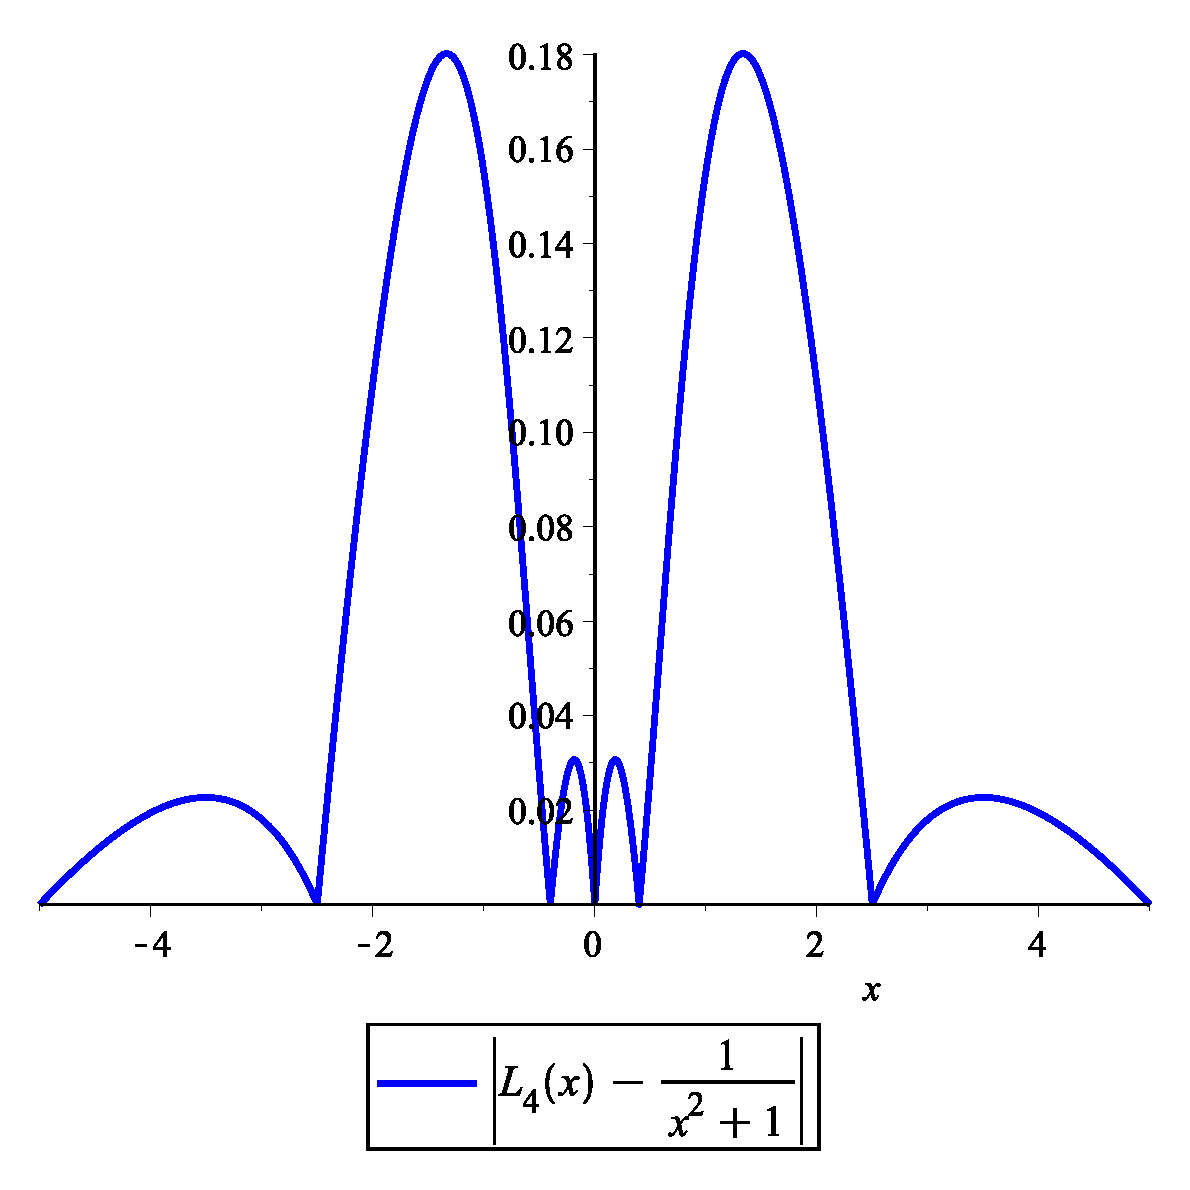
\includegraphics[scale=0.35]{err_L4.eps}
 \end{center}
\end{block}
}
%%%%
\frame{
\frametitle{Funci\'on de Runge $f(x) = \dfrac{1}{1+x^2}$}
\begin{block}{Error del interpolante lineal segmentaria 11 nodos.}
 \begin{center}
  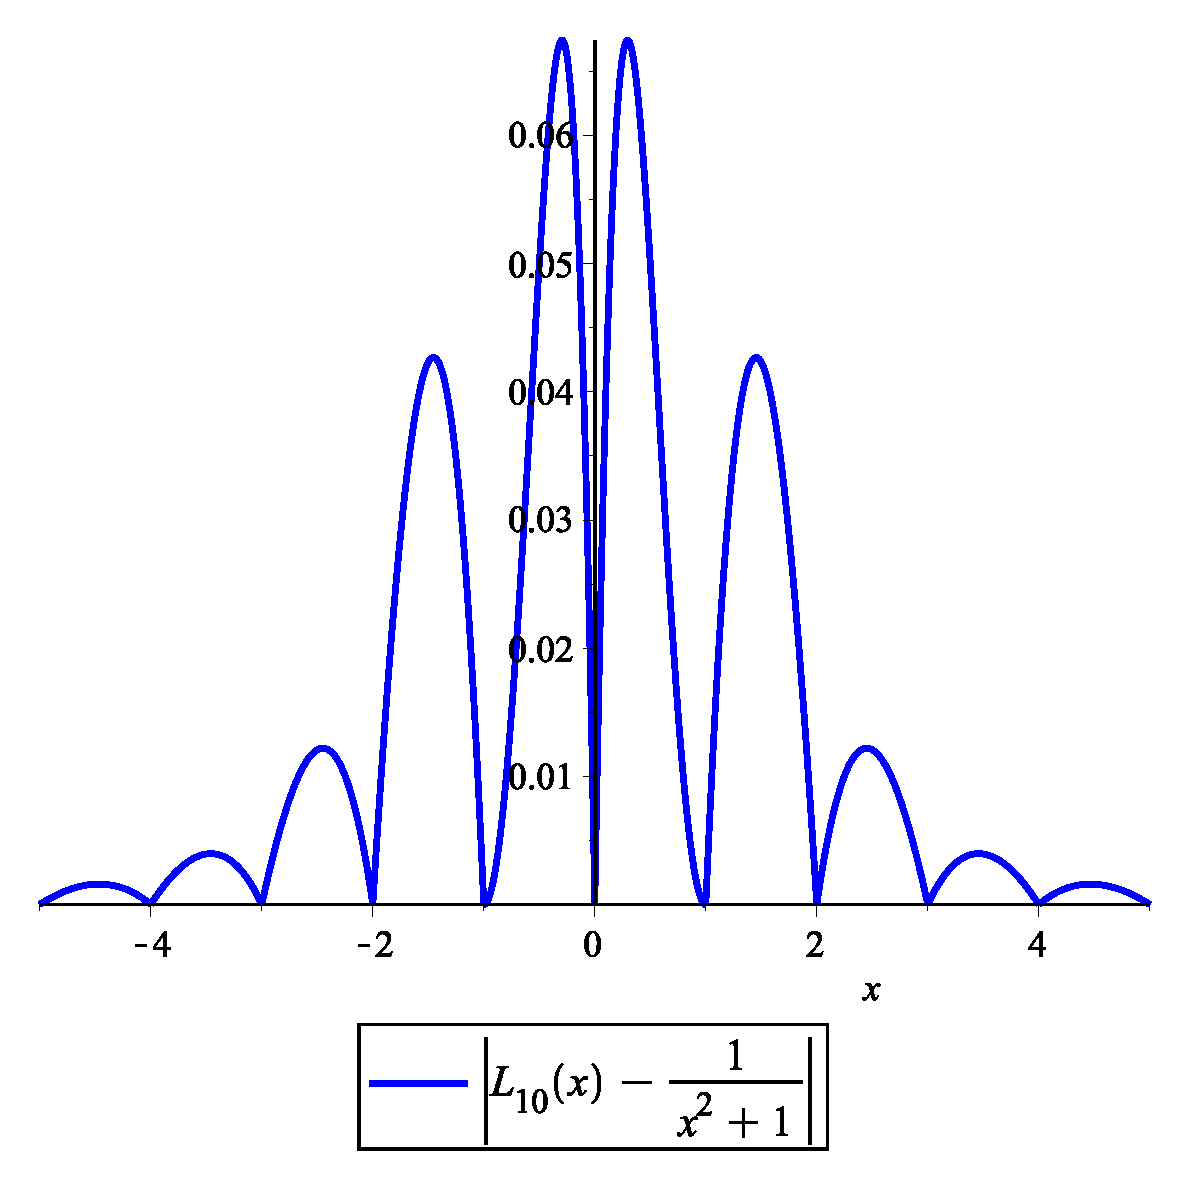
\includegraphics[scale=0.35]{err_L10.eps}
 \end{center}
\end{block}
}
%%%%
\frame{
\frametitle{Interpolaci\'on de Lagrange vs segmentaria}
\begin{block}{Coste de evaluaci\'on en un punto}
 \begin{itemize}
  \item Lagrange: se incrementa con el n\'umero de datos.
  \item<2-> Segmentaria: no crece con el n\'umero de nodos.
 \end{itemize}
\end{block}
\uncover<3->{
\begin{block}{Convergencia uniforme}
 \begin{itemize}
  \item Lagrange: no est\'a garantizado.
  \item<4-> Segmentaria: si
 \end{itemize}
\end{block}}
\uncover<5->{
\begin{block}{Derivabilidad}
 \begin{itemize}
  \item Lagrange: Indefinidamente derivable.
  \item<6-> Segmentaria: S\'olo continua.
\end{itemize}
\end{block}}
}
%%%%%%
\frame{
\frametitle{Interpolaci\'on Segmentaria C\'ubica}
\begin{itemize}
\item La interpolaci\'on segmentaria c\'ubica utiliza polinomios de tercer grado para cada subintervalo entre los puntos de datos.
\item<2-> Cada polinomio c\'ubico se ajusta de manera que no solo pase por los puntos de datos, sino que tambi\'en asegure que las primeras y segundas derivadas sean continuas en los puntos de uni\'on.
\item<3-> Esto resulta en una curva suave y continua que no presenta las oscilaciones que pueden ocurrir con polinomios de grado m\'as alto.
\item<4-> La forma general de un polinomio c\'ubico en el intervalo $[x_i, x_{i+1}]$ es:
$$
S_i(x) = a_i + b_i(x - x_i) + c_i(x - x_i)^2 + d_i(x - x_i)^3
$$
\item<5-> Los coeficientes $a_i, b_i, c_i, d_i$ se determinan imponiendo condiciones de continuidad y suavidad en los puntos de uni\'on.
\end{itemize}
}
%%%%%%
\frame{
\frametitle{Interpolaci\'on Segmentaria C\'ubica}
\begin{itemize}
\item Es posible construir una funci\'on c\'ubica $S_k(x)$ en cada intervalo $[x_k,x_{k+1}]$, tal que la curva a trozos $y = S(x)$ sea
dos veces diferenciable y $S(x)$ sea continua en $[x_0,x_n]$
\item<2-> lo primero implica que $y = f (x)$ no tiene esquinas y lo segundo que $S(x)$ tiene un radio de curvatura definido.
\item<3->Sea $f : [a, b] \to \mathbb{R}$ y sean $a = x_0 < x_1 < \cdots < x_n = b$. Un spline c\'ubico $S(x)$ para $f(x)$ es una funci\'on
que satisface:
\begin{enumerate}
 \item<4->$S_k(x)$ es un polinomio c\'ubico en cada intervalo $[x_k,x_{k+1}],\, \forall k=0,1,\ldots,n-1$.
 \item<5->$S_k(x_k) = f(x_k),\, k = 0, 1, \ldots, n$
 \item<6-> $S_k(x_{k+1}) = S_{k+1}(x_{k+1}),\, k = 0, 1,\ldots , n - 2$
 \item<7-> $S'_k(x_{k+1}) = S'_{k+1}(x_{k+1}),\, k = 0, 1,\ldots , n - 2$
 \item<8-> $S''_k(x_{k+1}) = S''_{k+1}(x_{k+1}),\, k = 0, 1,\ldots , n - 2$
\end{enumerate}
\end{itemize}
}
%%%%%%%
\begin{frame}
  \frametitle{Interpolaci\'on Segmentaria C\'ubica}

  Considerse los polinomios c\'ubicos
$$
S_k(x) = a_k + b_k(x - x_k) + c_k (x - x_k)^2 + d_k (x - x_k)^3 \quad \forall k=0,1,\ldots,n-1
$$

las dos primeras derivadas vienen dadas por
\begin{eqnarray}
 \nonumber S'_k(x) & = & b_k + 2c_k(x - x_k) + 3d_k(x - x_k)^2\\
 \nonumber S''_k(x) & = & 2c_k + 6d_k(x - x_k)
\end{eqnarray}

La condici\'on de que los splines pasen por los puntos de interpolaci\'on da 
$$
S_k(x_k) = a_k = y_k
$$
lo que dice que los coeficientes $a_k$ son los valores de la funci\'on interpolada en los nodos. 
\end{frame}
%%%%%%%
\frame{
\frametitle{Interpolaci\'on Segmentaria C\'ubica}
\begin{itemize}
\item El significado de los otros coeficientes es obviamente 
$$
S'_k(x_k) = b_k,\qquad S''_k(x_k) = 2c_k 
$$
  \item<2-> Las ecuaciones de continuidad de las funciones $S_k(x)$ y sus derivadas primera y segunda en los $n - 1$ puntos de interpolaci\'on intermedios $x_{k+1}, k = 0,\ldots, n - 2$ (las condiciones de continuidad no se aplican a los extremos) dan
\begin{eqnarray}
 \nonumber a_{k+1} & = & a_k + b_k(x_{k+1} - x_k) + c_k(x_{k+1} - x_k)^2 + d_k(x_{k+1} - x_k)^3\\
 \nonumber b_{k+1} & = & b_k + 2c_k(x_{k+1} - x_k) + 3d_k(x_{k+1} - x_k)^2\\
 \nonumber 2c_{k+1} & = & 2c_k + 6d_k(x_{k+1} - x_k)
\end{eqnarray}
\end{itemize}
}
%%%%%%%
\frame{
\frametitle{Interpolaci\'on Segmentaria C\'ubica}
\begin{itemize}
\item Esto constituye un sistema de $3(n - 1)$ ecuaciones para determinar los $3n$ coeficientes $b_k$, $c_k$ y $d_k$.
\item<2->Una condici\'on adicional es que el \'ultimo spline pase por el \'ultimo punto: $S_{n-1}(x_n) = y_n$.
\item<4-> Se requieren por tanto dos condiciones adicionales para poder determinar todos los coeficientes. 
\item<5->Para simplificar la notaci\'on, sea  $h_k = x_{k+1} - x_k$. De esta manera se pueden escribir las ecuaciones de continuidad anteriores como
\begin{eqnarray}
 \nonumber \dfrac{a_{k+1} -a_k }{h_k} & = &  b_k + c_kh_k + d_kh_k^2\\
 \nonumber b_{k+1} - b_k & = &  2c_kh_k + 3d_kh_k^2\\
 \nonumber c_{k+1}- c_k & = & 3d_kh_k
\end{eqnarray}
\end{itemize}
}
%%%%%%%
\frame{
\frametitle{Interpolaci\'on Segmentaria C\'ubica}
\begin{itemize}
\item<1-> De las posibles formas de resolver el sistema de ecuaciones anterior, la m\'as comoda es despejar los coeficientes 
$d_k$ y $b_k$ de forma que se obtenga un sistema de ecuaciones para los coeficientes $c_k$.
\item<2->Si se despeja
$$
d_k = \dfrac{c_{k+1}- c_k}{3h_k}
$$
en la \'ultima ecuaci\'on y se introduce en la segunda ecuaci\'on, se obtiene
$$
 b_{k+1} - b_k =   2c_kh_k + 3\left(\dfrac{c_{k+1}- c_k}{3h_k}\right)h_k^2 = (c_k + c_{k+1})h_k
$$
\end{itemize}
}
%%%%%%%
\frame{
\frametitle{Interpolaci\'on Segmentaria C\'ubica}
\begin{itemize}
\item Se necesita otra expresi\'on independiente de $b_{k+1} - b_k$ para obtener una ecuaci\'on para los $c_k$.
\item<2->En la primera de las ecuaciones se puede despejar $b_k$ 
$$
b_k = \dfrac{a_{k+1} -a_k}{h_k} - c_kh_k - d_kh_k^2 = \dfrac{a_{k+1} -a_k}{h_k} - c_kh_k -\left(\dfrac{c_{k+1}- 
c_k}{3h_k}\right) h_k^2 
$$
$$
= \dfrac{a_{k+1} -a_k}{h_k} -\dfrac{2}{3}c_kh_k -\dfrac{1}{3}c_{k+1}h_k
$$
y cambiando $k$ por $k + 1$ se obtiene
$$
b_{k+1} = \dfrac{a_{k+2} -a_{k+1}}{h_{k+1}} -\dfrac{2}{3}c_{k+1}h_{k+1} -\dfrac{1}{3}c_{k+2}h_{k+1}
$$
\end{itemize}
}
%%%%%%%
\frame{
\frametitle{Interpolaci\'on Segmentaria C\'ubica}
\begin{itemize}
\item<1-> Restando estas dos ecuaciones queda
$$
b_{k+1} - b_k = 
$$
$$
\dfrac{a_{k+2} -a_{k+1}}{h_{k+1}} - \dfrac{a_{k+1} -a_k}{h_k} - \dfrac{1}{3}c_{k+2}h_{k+1} 
 + \dfrac{1}{3}c_{k+1}h_k - \dfrac{2}{3}c_{k+1}h_{k+1} + \dfrac{2}{3}c_kh_k
$$
\item<2->Igualando ambas expresiones se obtiene una relaci\'on entre los $c_k$:
$$
\dfrac{1}{3}c_{k+2}h_{k+1} + \dfrac{2}{3}c_{k+1}(h_k+h_{k+1}) + \dfrac{1}{3}c_kh_k = \dfrac{a_{k+2} -a_{k+1}}{h_{k+1}} 
- \dfrac{a_{k+1} -a_k}{h_k}
$$
\end{itemize}
}
%%%%%%%
\frame{
\frametitle{Interpolaci\'on Segmentaria C\'ubica}
\begin{itemize}
\item Estas ecuaciones forman un sistema tridiagonal. Si se define
$$
v_{k+1} = 3\left(\dfrac{a_{k+2} -a_{k+1}}{h_{k+1}} - \dfrac{a_{k+1} -a_k}{h_k}\right)
$$
\item<2-> El sistema tridiagonal queda como
$$
c_{k+2}h_{k+1} + 2c_{k+1}(h_k + h_{k+1}) + c_kh_k = v_{k+1}
$$
\end{itemize}
}
%%%%%%%
\frame{
\frametitle{Interpolaci\'on Segmentaria C\'ubica}
\begin{itemize}
\item<1-> Dondo la matriz de coeficientes es:
\footnotesize{
$$
 \left[\begin{array}{ccccccc}
       h_0 & 2(h_0+h_1) & h_1 & 0 & 0 & \cdots & 0\\
       0 & h_1 & 2(h_1+h_2) & h_2 & 0 & \cdots & 0\\
       0 & 0 & h_2 & 2(h_2+h_3) & h_3 &  \cdots & 0\\
       0 & 0 & 0 & h_3 & 2(h_3+h_4) & \cdots & 0\\
       \vdots & \vdots & \vdots & \vdots & \vdots & \vdots & \vdots\\
       0 & 0 & 0  & \cdots & h_{n-3} & 2(h_{n-3}+h_{n-2}) & h_{n-2}
      \end{array}\right]
$$}
\item<2->Y vector de inc\'ognitas y t\'erminos independientes
$$
\left[\begin{array}{c}
  c_0\\
  c_1\\
  c_2\\
  \vdots\\
  c_{n-2}\\
  c_{n-1}
 \end{array}\right] ,\qquad \left[\begin{array}{c}
  v_1\\
  v_2\\
  v_3\\
  \vdots\\
  v_{n-3}\\
  v_{n-2}
 \end{array}\right]
$$
\end{itemize}
}
%%%%%%%
\frame{
\frametitle{Interpolaci\'on Segmentaria C\'ubica}
\begin{itemize}
\item<1-> Este es un sistema de $n - 2$ ecuaciones para $n$ inc\'ognitas.
\item<2->Se necesitan dos ecuaciones adicionales para determinar 
los $c_k$.
\item<3->Estas dos ecuaciones se proporcionan mediante dos condiciones en cierta forma arbitrarias, pero de las que 
depende la calidad del ajuste.
\end{itemize}
}
%%%%%%%
\frame{
\frametitle{Interpolaci\'on Segmentaria C\'ubica}
\begin{center}
  \bf Condiciones Naturales
\end{center}
\begin{block}{Teorema}
  Sea $f(x)$ una funci\'on definida en $[x_0, x_n]$. Entonces existe un \'unico $S(x)$ spline interpolante c\'ubico para $f(x)$ en $[x_0, x_n]$ tal que $S''(x_0) = 0$ y $S''(x_n) = 0$.
\end{block}
\begin{align*}
  c_n = S''(x_n)/2 = 0 &\to c_n = 0\\
  S''(x_0) = 2c_0 = 0 &\to c_0 = 0
\end{align*}
\begin{itemize}
  \item<2-> El coeficiente $c_n$ no pertenece a ninguno de los splines en $[x_0, x_n]$, sino a un spline arbitrario que comienza en el extremo $x_n$, pero la introducci\'on de $S_n(x)$ permite extender las ecuaciones para los coeficientes $c_k$ con una ecuaci\'on adicional
  $$
  h_{n-2} c_{n-2} + 2(h_{n-2} + h_{n-1})c_{n-1} = v_{n-1}
  $$
\end{itemize}
}
%%%%%%%
\frame{
\frametitle{Interpolaci\'on Segmentaria C\'ubica}
\begin{itemize}
\item<1-> La condici\'on $c_0 = 0$ permite eliminar la primera columna de la matriz del sistema.
\item<2-> Con estas dos modificaciones, el sistema de ecuaciones queda de la forma:
\end{itemize}
\uncover<2->{
\footnotesize{
$$
\left[\begin{array}{cccccc}
  2(h_0+h_1) & h_1 & 0 & 0 & \cdots & 0\\
  h_1 & 2(h_1+h_2) & h_2 & 0 & \cdots & 0\\
  0 & h_2 & 2(h_2+h_3) & h_3 &  \cdots & 0\\
  0 & 0 & h_3 & 2(h_3+h_4) & \cdots & 0\\
  \vdots & \vdots & \vdots & \vdots & \vdots & \vdots\\
  0 & 0  & \cdots & h_{n-3} & 2(h_{n-3}+h_{n-2}) & h_{n-2}\\
  0 & 0  & 0 & \cdots & h_{n-2} & 2(h_{n-2}+h_{n-1})\\
 \end{array}\right]
$$
$$
\left[\begin{array}{c}
  c_1\\
  c_2\\
  c_3\\
  \vdots\\
  c_{n-2}\\
  c_{n-1}
 \end{array}\right] = \left[\begin{array}{c}
  v_1\\
  v_2\\
  v_3\\
  \vdots\\
  v_{n-2}\\
  v_{n-1}
 \end{array}\right]
$$}
que es un sistema de $n - 1$ ecuaciones con $n - 1$ inc\'ognitas.}
}
%%%%
\frame
{
\frametitle{Ejemplo:}
Aproximar la funci\'on $f(x)=\frac{1}{1+x^2}$, empleando interpolaci\'on sobre el soporte formado por los puntos:
\scriptsize
$$
(-4.0, 0.05882352941), (-2.0, 0.2), (0.0, 1.0), (1.0, 0.5), (2.0, 0.2), (4.0, 0.05882352941)
$$
\normalsize
\uncover<2->{Polinomio de Interpolaci\'on de Lagrange
$$
1.0 -0.3764x - 0.2470x^2 + 0.1176x^3 + 0.01176x^4 - 0.005882x^5
$$}
}
%%%%
\frame
{
$$
\begin{array}{cc}
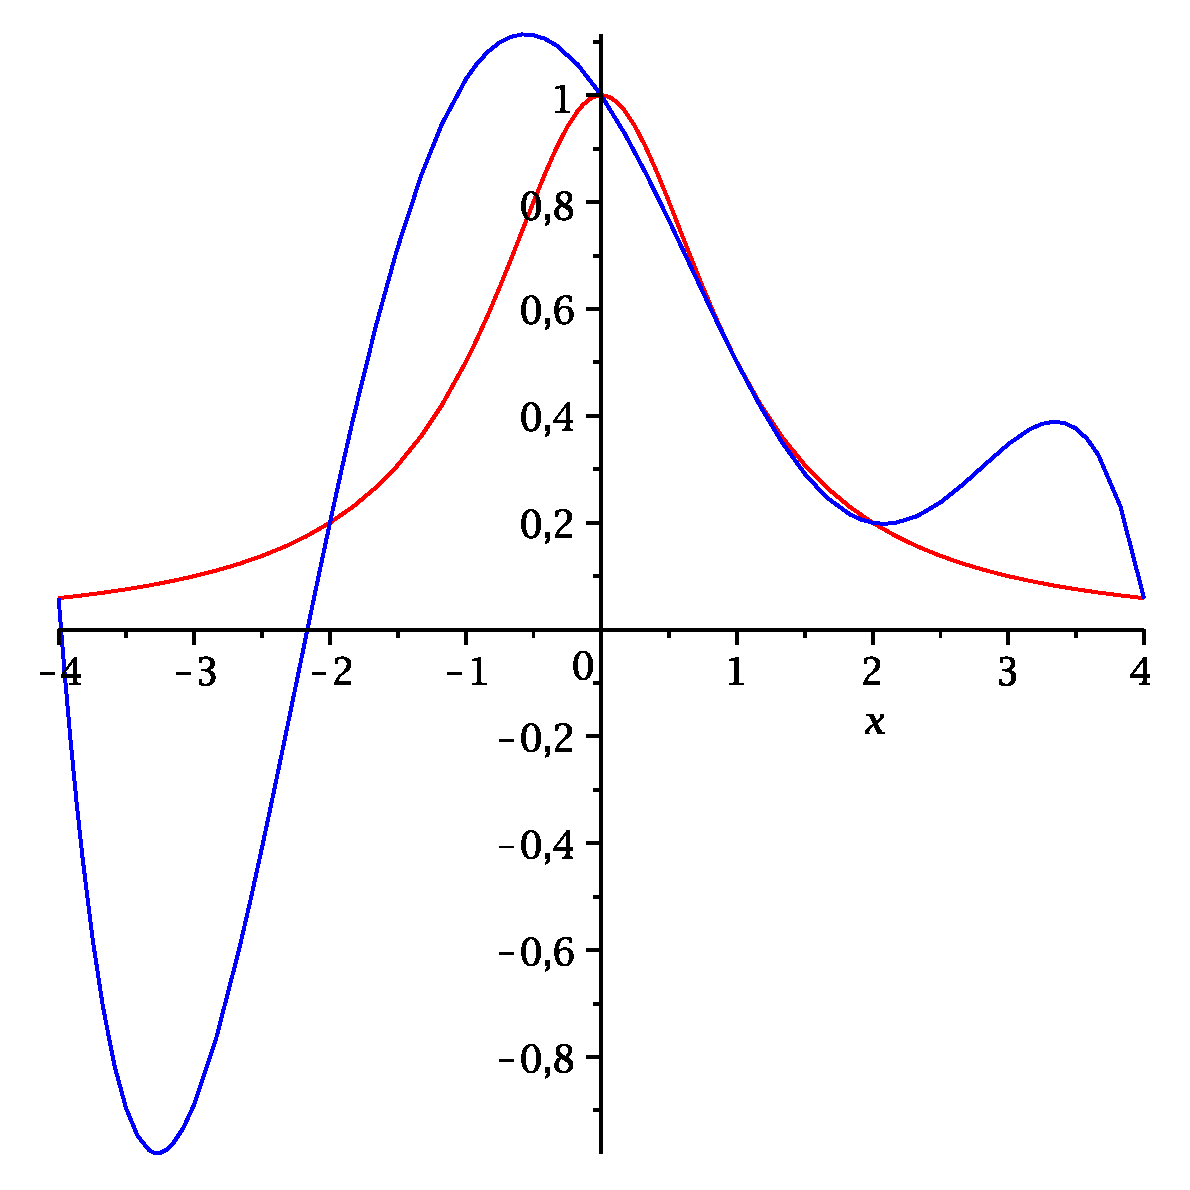
\includegraphics[scale=0.23]{lagrange.eps} & 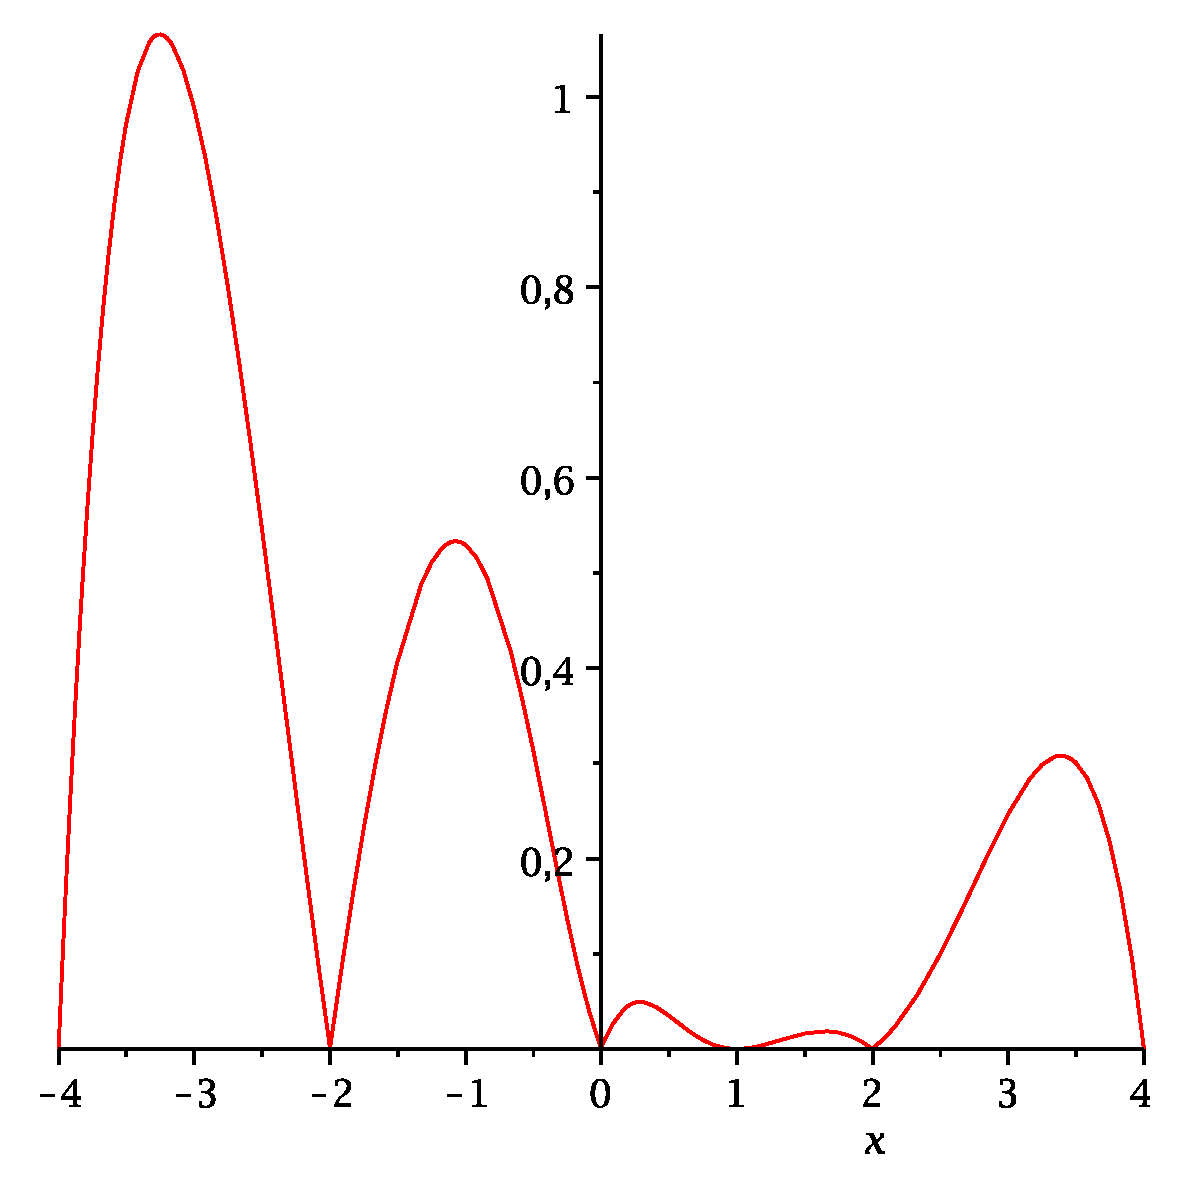
\includegraphics[scale=0.23]{errorlagrange.eps}\\
\textcolor{red}{\frac{1}{1+x^2}} \text{ vs }\textcolor{blue}{P_5(x)} & |E(x)|=|f(x)-P_5(x)| 
\end{array}
$$
}
%%%%
\frame
{
Spline c\'ubico
$$
S(x) = \left\{
\begin{array}{ll}
2.502 + 2.052x + 0.5403x^2 + 0.04503x^3 & x<-2.0\\
1.0 - 0.2020x - 0.5866x^2 - 0.1428x^3 & x<0.0\\
1.0 - 0.2020x - 0.5866x^2 + 0.2887x^3 & x<1.0\\
1.359 - 1.279x + 0.4911x^2 - 0.07051x^3 & x<2.0\\
0.8859 - 0.5699x + 0.1361x^2 - 0.01134x^3 & x\geq 2.0
\end{array}\right. 
$$
}
%%%%
\frame
{
$$
\begin{array}{cc}
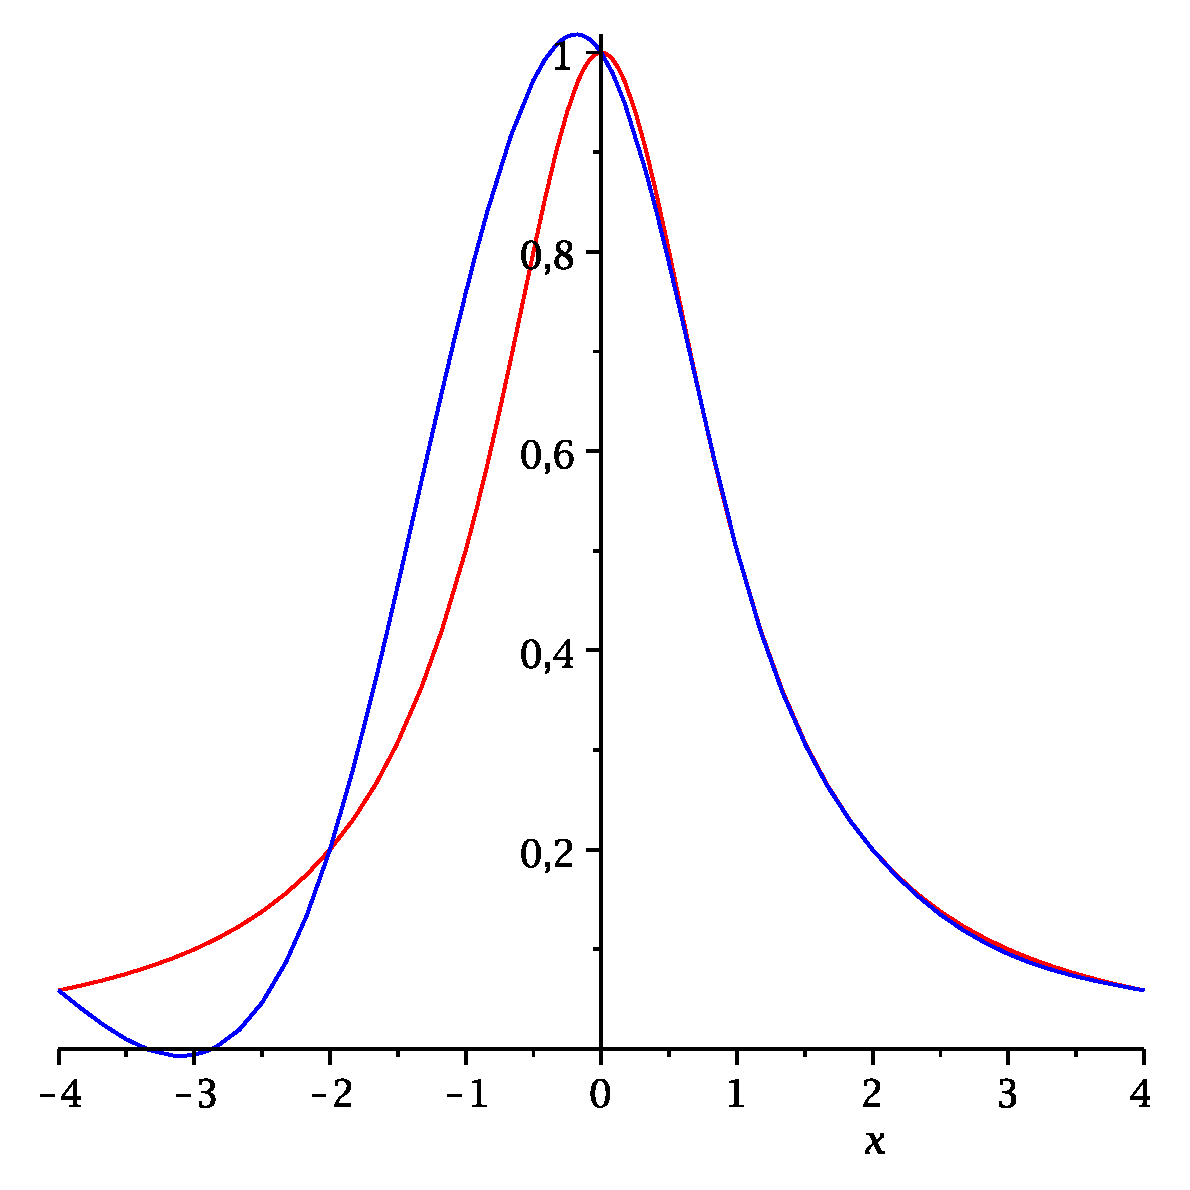
\includegraphics[scale=0.23]{spline.eps} & 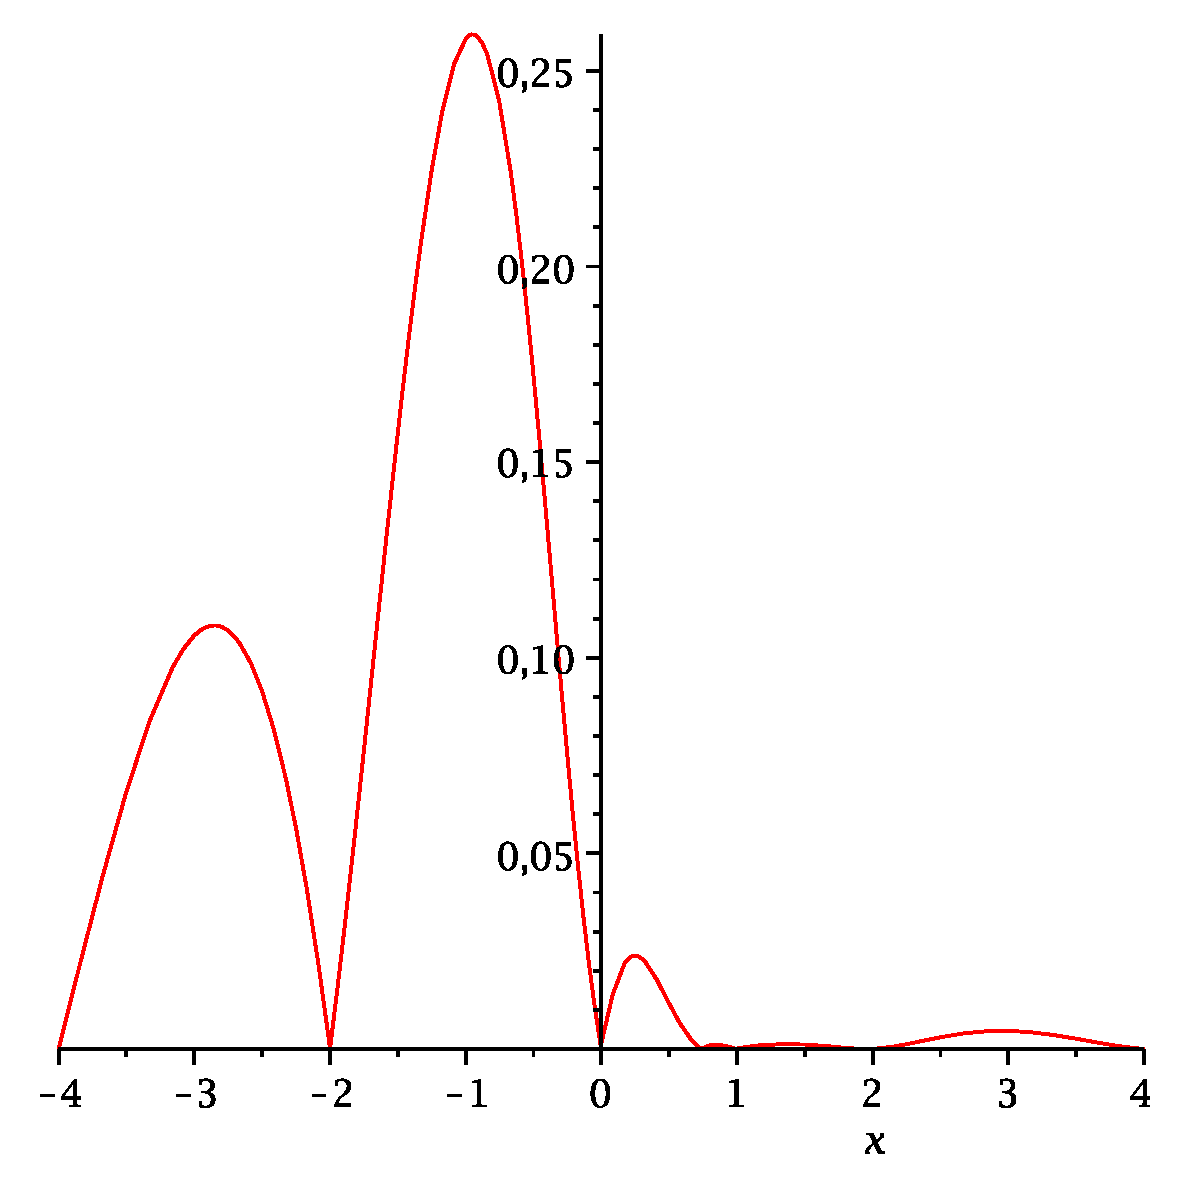
\includegraphics[scale=0.23]{errorspline.eps}\\
\textcolor{red}{\frac{1}{1+x^2}} \text{ vs }\textcolor{blue}{S(x)} & |E(x)|=|f(x)-S(x)| 
\end{array}
$$
}
%%%
\frame
{
\frametitle{Condiciones Sobre la Derivada}
\begin{block}{Teorema}
Sea $f(x)$ una funci\'on definida en $[x_0,x_n]$. Entonces existe un \'unico $S(x)$ spline c\'ubico interpolante para $f(x)$ en $[x_0,x_n]$, tal que:
$$
                S'(x_0) =  f'(x_0)      \text{  y  }           S'(x_n) = f'(x_n).
$$
\end{block}

\begin{eqnarray}
2h_0c_0 + h_0c_1 & = & \frac{3}{h_0}(a_1 - a_0 ) - 3f'(x_0)\nonumber\\
h_{n-1}c_{n-1} + 2h_{n-1}c_n & = & 3f'(x_n) - \frac{3}{h_{n-1}} (a_n - a_{n-1})\nonumber
\end{eqnarray}
}
%%%%
\frame
{
\frametitle{Condiciones Sobre la Derivada}
A\~nadiendo al sistema de ecuaciones que determina los $c_k$ las dos ecuaciones adicionales, se tiene que los $c_k$ vienen dados por la soluci\'on de un sistema de $n + 1$ ecuaciones con $n + 1$ inc\'ognitas:
{\scriptsize
$$
 \left[\begin{array}{cccccc}
       2h_0 & h_0 & 0 & 0 & \cdots & 0\\
       h_0 & 2(h_0+h_1) & h_1 & 0 & \cdots & 0\\
       0 & h_1 & 2(h_1+h_2) & h_2 &  \cdots & 0\\
       0 & 0 & h_2 & 2(h_2+h_3) & \cdots & 0\\
       \vdots & \vdots & \vdots & \vdots & \vdots & \vdots\\
       0 & 0  & \cdots & h_{n-2} & 2(h_{n-2}+h_{n-1}) & h_{n-1}\\
       0 & 0  & 0 &\cdots & h_{n-1} & 2h_{n-1}\\
      \end{array}\right]$$
      $$\left[\begin{array}{c}
                               c_0\\
                               c_1\\
                               c_2\\
                               \vdots\\
                               c_{n-1}\\
                               c_n
                              \end{array}\right] = \left[\begin{array}{c}
                               v_0\\
                               v_1\\
                               v_2\\
                               \vdots\\
                               v_{n-1}\\
                               v_n
                              \end{array}\right]
$$}
con
\begin{eqnarray}
\nonumber v_0 & = & 3\left(\dfrac{a_1 - a_0}{h_0}-f'_0\right)\\
\nonumber v_n & = & 3\left(f'_n -\dfrac{a_n - a_{n-1}}{h_{n-1}}\right)
\end{eqnarray}
}
%%%%
\frame
{
  \frametitle{Ejemplo:}
Spline c\'ubico
$$
S(x) = \left\{
\begin{array}{ll}
2.765 + 2.452x + 0.7255x^2 + 0.07040x^3 & x<-2.0\\
1.0 - 0.1964x - 0.5988x^2 - 0.1503x^3 & x<0.0\\
1.0 - 0.1964x - 0.5988x^2 + 0.2952x^3 & x<1.0\\
1.374 - 1.318x + 0.5232x^2 - 0.07875x^3 & x<2.0\\
0.7472 - 0.3784x + 0.05319x^2 - 0.0004064x^3 & x\geq 2.0
\end{array}\right. 
$$
}
%%%%
\frame
{
  \frametitle{Ejemplo:}
$$
\begin{array}{cc}
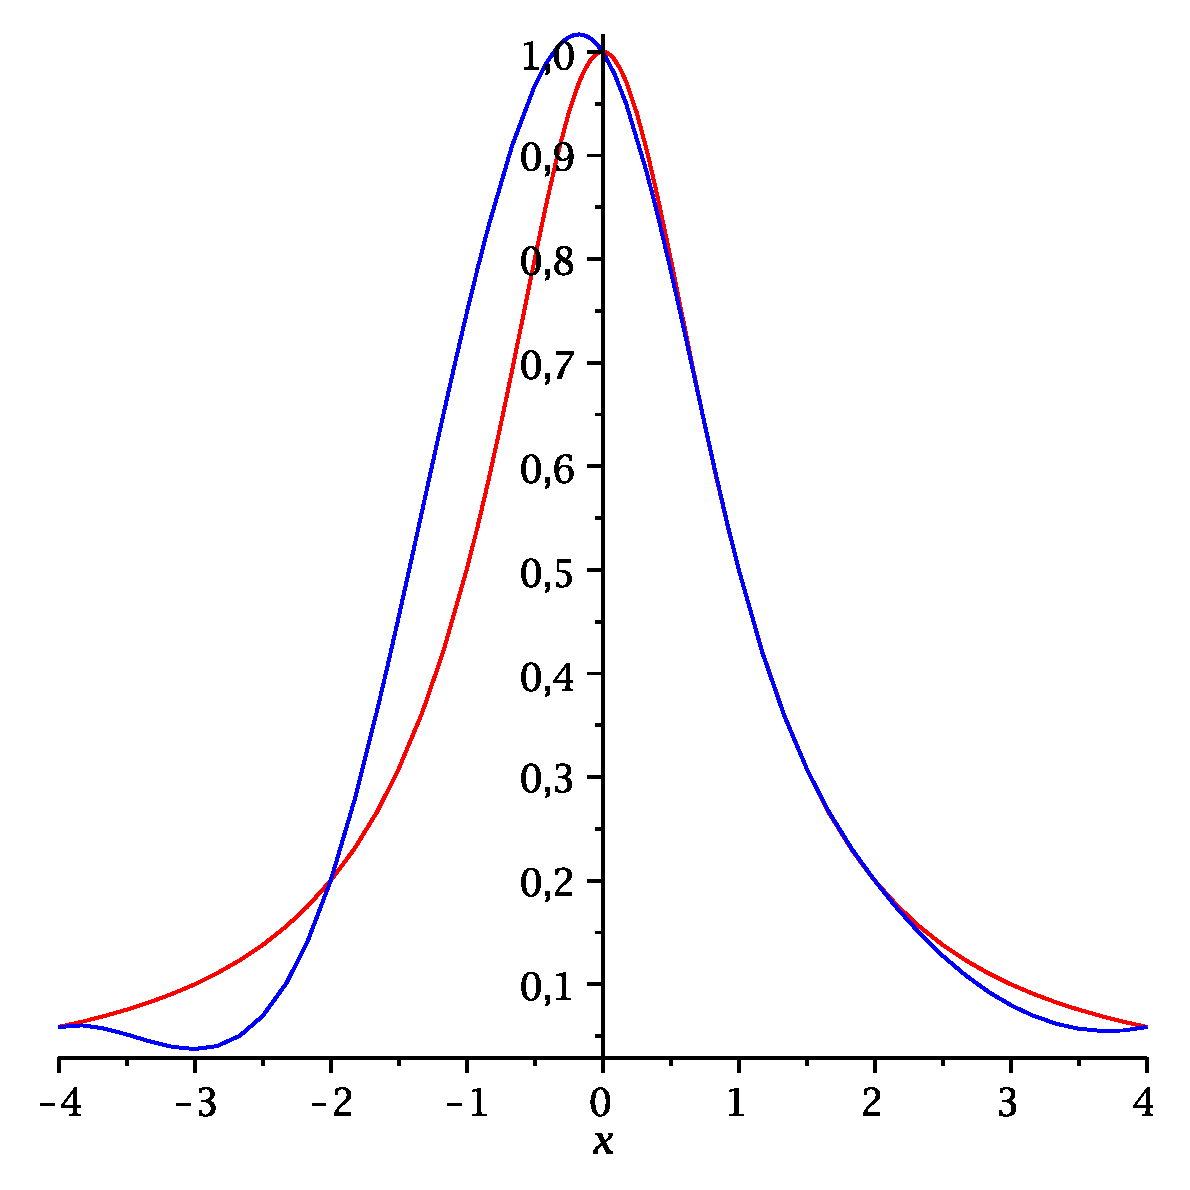
\includegraphics[scale=0.23]{splineder.eps} & 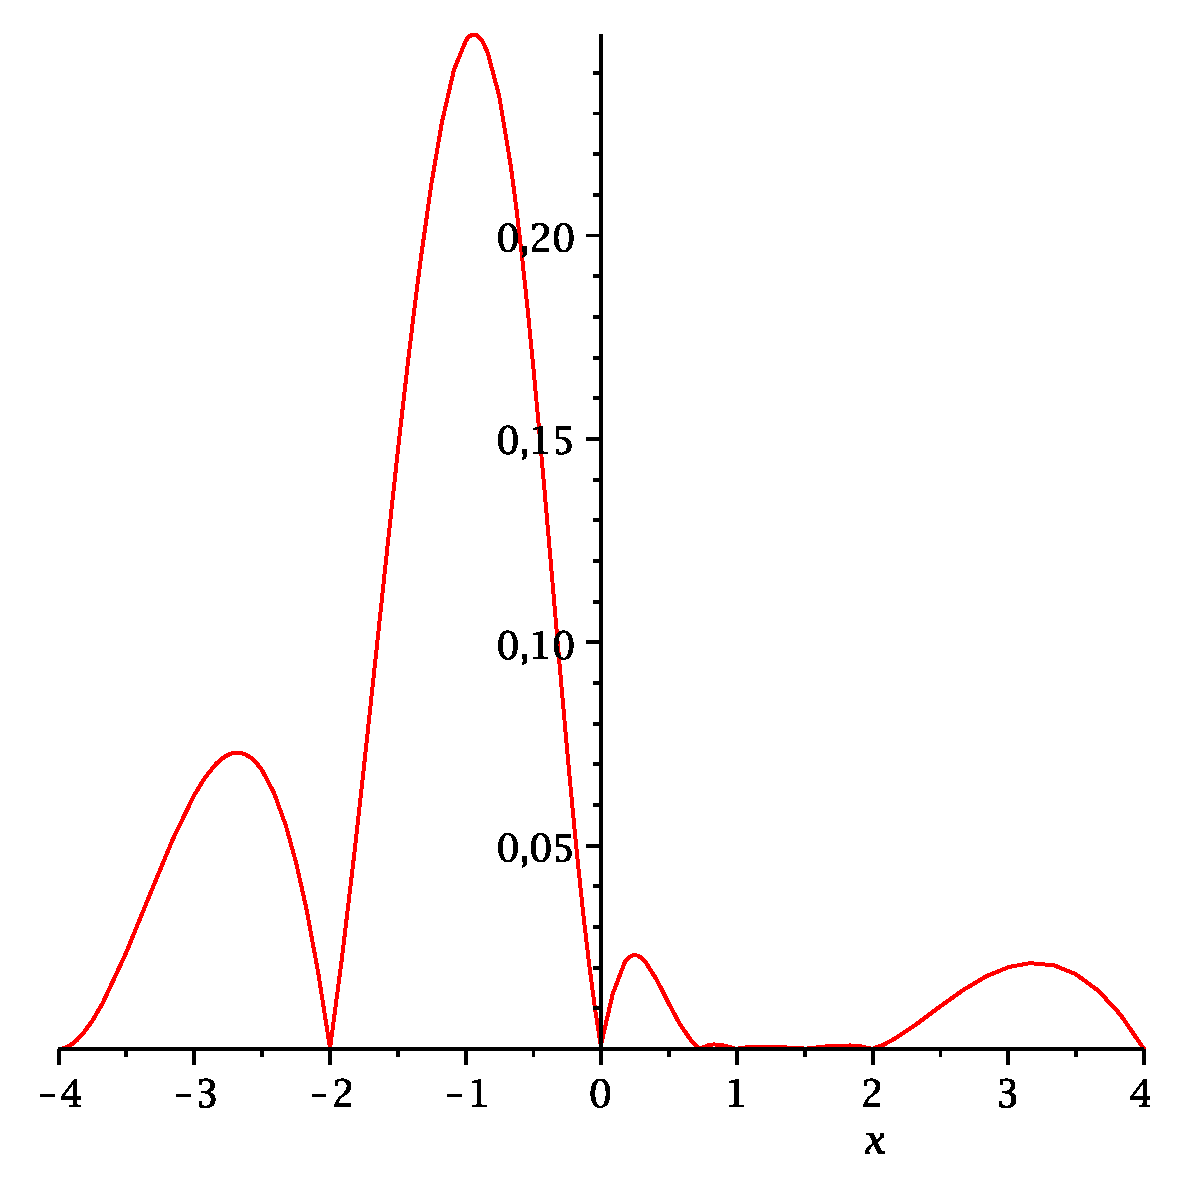
\includegraphics[scale=0.23]{errorsplineder.eps}\\
\textcolor{red}{\frac{1}{1+x^2}} \text{ vs }\textcolor{blue}{S(x)} & |E(x)|=|f(x)-S(x)| 
\end{array}
$$
}
\end{document}